\let\textcircled=\pgftextcircled
\chapter{Markov State Model Optimization}
\label{chap:msm}

\section{Introduction}
Computational chemistry and physics are becoming increasingly reliant on complex statistical and machine learning models to understand the high dimensional datasets [Noe review]. Markov state models (MSMs) are used to characterise the metastable conformational dynamics of large biomolecules using a suitably processed set of molecular dynamics (MD) trajectories [ref]. The processing pipeline involves choosing potentially $10$s of model hyperparameters in the following four broad steps [ref]:

\begin{enumerate}
    \item \textbf{Featurization:} choosing a set of features of the biomolecule, such as the residue contact distances, into which to transform the Cartesian coordinates of the MD trajectories. 
    \item \textbf{Dimensionality reduction:} using PCA or TICA  to rotate, scale and project the featurized trajectories into a suitable subspace ready for discretization.  
    \item \textbf{Discretization:} further projecting the trajectories into a discrete set of microstates to estimate the MSM transition matrix. 
    \item \text{Coarse graining:} mapping microstates into larger metastable macrostates to aide interpretability.   
\end{enumerate}

Even with a modest number of hyperparameters the space of choices available is huge.  Features($\chi$) used in biomolecular MSMs include, but are not limited to, protein backbone torsions [ref], residue torsions [ref], residue contact distances[ref] and root mean square deviation of various subsets of atom positions [ref]. Using TICA one has to choose a lag time ($\tau$ \footnote{note: this is not the MSM lag time (also denoted $\tau$) and is not a hyperparameter but specifies the MSM itself. This cannot be optimized [] and I consider it fixed for a given system throughout this chapter.}) and the number of independent components to retain ($m$). Additionally one may also choose to scale the components by functions of the TICA eigenvalues so that distances in the new space correspond to kinetic [] or commute distances []. Discretization involves choosing the number of microstates ($n$) and the clustering algorithm which has been shown to have a significant effect on the final model parameters [ref].  The choices involved in coarse graining, such as the final number of metastable states and the method used for coarse graining will be discussed in chapter \ref{chap:hmm}. 

Finding the `best' set of hyperparameters, $\mathbf{\lambda}$, for a given model is a common task in machine learning[ref]. Typically the optimum value of $\mathbf{\lambda}$ is chosen to optimise an objective function, e.g.root mean square error [ref] on unseen data. In the case of MSMs, the optimum is given by the maximum of the cross-validated $\operatorname{VAMP-r}$ score, hereafter denoted $f(\cdot)$, as discussed in chapter \ref{chap:theory}. In order to find the value of $\mathbf{\lambda}$ which maximizes $f$ there are a number of different hyperparameter optimisation techniques available, but which fall into two categories. 

\emph{Exhaustive search} [ref] involves scoring a set of  hyperparameters trials chosen from either an regular grid or at random from the hyperparameter space. The best performing trial is then taken from this set. For all but the most simple of hyperparameter spaces, random search has been shown [] to more efficient than  than grid search. The reason is that some hyperparameters are more relevant than others in determining the objective function. Grid search places equal importance on each hyperparameter and effectively wastes the trial `budget' (the number of trials scored) on combinations of hyperparameter which will score similarly. 

\emph{Model based} searches involve estimating the response surface of the model and using this information to choose the next trial. The response surface is the function which maps the hyperparameters to the objection function, given a set of training data. In the case of MSMs, the response surface is the value of $f$ as a function of $\chi$, $\tau$, $m$, $n$ etc. given a set of molecular dynamics trajectories, $\mathbf{x}$: $f(\lambda; \mathbf{x})$ \footnote{The dependence on $\mathbf{x}$ will be assumed from now on. }. A popular model based technique is Bayesian optimisation, described in section \ref{sec:BO} of chapter \ref{chap:theory}. Bayesian optimisation have been used in various hyperparameter optimisation tools [bayesopt, osprey].  The key components of Bayesian optimisation are the surrogate function, which models the response surface, and the acquisition function, which determines how current knowledge and uncertainty of the response surface is mapped to candidate hyperparameter trials. 

Gaussian processes (GPs) have been used as a surrogate function for Bayesian optimisation[ref] and have many useful properties. First, many common acquisition functions are simple functions of the parameters of the fitted GP model [ref]. Second, they do not assume specific mappings between predictor and response (e.g. linear, quadratic etc.). Rather, they specify the structure of the covariance between values of the response as a function of predictors through a kernel function $k(\lambda, \lambda')$ [ref]. This allows easy fitting of arbitrarily shaped response functions.  With recent work [ref] in approximate estimation methods they are also able to handle large data sets. In addition to their usefulness in Bayesian optimisation, the estimated parameters of the GP models of the response surface are interpretable and provide insight into the relevance of hyperparameters and how they interact.  For example, in [Bergstra] they were able to show that the learning rate was consistently the most important hyperparameter for determining accuracy of neural networks for classifying digits. 


Thus GPs are central to both understanding the response function of machine learning models and to optimising their performance. To use them effectively the kernel function and other modelling steps, such as transformations of the predictor variables, must be appropriately specified. These will in general be specific to the type of machine learning model being optimised.  In this work  I will use Gaussian processes in order to both optimize MSMs and to understand which hyperparameters are relevant to maximizing $\operatorname{VAMP-r}$.  In particular I will answer the following questions: 

\begin{enumerate}
    \item ?
    \item ?
\end{enumerate}

This chapter is structured as follows. In section xx I estimate the response surface of Alanine dipeptide (Ala-1), a well known test system for benchmarking methods in molecular kinetics. In subsection xx I discuss how I modelled this as a GP and how to use the GP model to estimate and interpret the relevance of the MSM hyperparameters. Finally for Alanine dipeptide, in subsection xx, I demonstrate how to use Bayesian optimisation to optimise the hyperparameters and discuss the impact of the optimisation on other observables of the MSM. 

I then apply the lessons learned in understanding and optimising Ala-1, to the conformational dynamics of the active site of Aromatic Amine Dehydrogenase (AADH) in section xxx. 



% The researcher interested applying such techniques to their system of interest must make a number of analytical choices, or hyperparameters, about the training process which materially impact the fitted model and thus the scientific inferences that can be drawn. Understanding how hyperparameters affect the model outcome is important for ensuring the robustness and reproducibility of the scientific conclusions derived from them. Armed with this knowledge it is also possible to choose hyperparameters which are optimal in some way. However, even with a small number of hyperparameters the space of all combinations of hyperparameters suffers from the curse of dimensionality and thus requires substantive experimentation to understand and optimize. 

% Within the machine learning practice and literature there has been much development on methods for tuning hyperparameters. This tuning consists of selecting a vector of hyperparameters relevant to the model being used, $\lambda$, training a model on data $X$, evaluating some objective function $\mathcal{L}(\lambda,X)$ and repeating until a suitable minimum (or maximum) $\mathcal{L}$ has been achieved. A successful tuning algorithm therefore selects a sequence of $\lambda$ which quickly converges on the global minimum $\mathcal{L}$. Bergstra and Bengio ([]) showed that selecting values of $\lambda$ at random is superior to selecting values from an evenly spaced grid of points for deep learning models for image recognition. The explanation was that grid search places equal importance on each combination of hyperparameters, while in practice only a small subset are important. In order to demonstrate this, they randomly selected a sequence of $\lambda_i$ evaluated the loss, $\mathcal{L}_i$, and used Gaussian Processes regression (GPR) to understand the importance of each element of $\lambda$ in determining the loss. This mapping, $\mathcal{L}=\Psi(\lambda, X)$, is known as the response surface of the model. GPR models are particularly suited to modelling the response surface as they are flexible in modelling different data types, they model both mean response and its uncertainty, can fit within a fully Bayesian inference framework, and there exist efficient approximate methods to cope with large datasets. 

% Tuning algorithms have since improved through the use of Bayesian Optimization which uses the response surface to suggest values of $\lambda_i$ which take into account both knowledge of where the loss is likely to be small and how certain we are that this is the case, the so-called exploit/explore trade-off. In the early stages of tuning where uncertainty is high, Bayesian optimization can be made to explore the space of hyperparameters to build up an accurate response surface model and then in the later stages, to exploit this knowledge to try regions of hyperparameter space which are likely to yield small values of L. 


	


% \section{Theory}
% \subsection{Markov State Models}
% Markov State Models (MSMs) have been used extensively to model protein dynamics. A MSM discretizes the configurational space of the protein into n discrete basis functions and models the dynamics, $x(t)$ of the protein as stochastic jumps, after some time, $\tau^MSM$, between these states with a given conditional probability $T_ij=P(x(t+\tau^MSM )=j|x(t)=i)$. These matrix elements are estimated from molecular dynamics data, $X$, after suitable pre-processing. This pre-processing can take different forms but typically this will entail: 
% \begin{enumerate}
%     \item Projecting the cartesian coordinates on a relevant feature, $\chi$, of smaller dimension, e.g. protein backbone torsions.
%     \item Reducing the dimensionality further by a linear approximation to the transition matrix known as time-lagged independent component analysis (TICA). This operation is parameterized by a time lag ($\tau$) and the number of TICA components ($m$) to retain. 
%     \item Discretizing the new m-dimensional space into $n$ discrete clusters, which form the basis for the MSM. 
% \end{enumerate}

% The analytical choices can be summarised in the hyperparameter vector $\lambda=(\chi,\tau,m,n)$. The metastable dynamics of the protein reveal themselves through the separation of the eigenvalues of  $T$ into $k$ values close to $1$, which give rise to the slow dynamics, and $n-k$ small values which determine the fast dynamics. The usual objective functions for MSMs are based on maximizing the sum of the $k$ largest eigenvalues of $T$ (known as the GMRQ or VAMP-1 score). 

% \subsection{Gaussian Processes Regression}
% \subsubsection{Gaussian process}
% A Gaussian process is a collection of Gaussian random variables, indexed by a variable x, with means m(x) and covariance specified by a kernel, $k(x,x')$ [RW]. Any finite subset of these is equivalent to a draw from a multivariate normal distribution (MVN). We may consider the response function as a Gaussian process, i.e. we can identify the GMRQ ($y$) as a draw from the multivariate normal indexed by the hyperparameter vector $\lambda$: $y=f(\lambda)= MVN(m(\lambda),k(\lambda,\lambda'))$ where the prime indicates all other possible values of $\lambda$. 

% \subsubsection{Gaussian Processes regression}


% \subsection{Bayesian Optimization}

\section{Methods}\label{sec:methods}
\subsection{Molecular dynamics}
This work uses the response surface of MSMs built on two systems: alanine dipeptide (Ac-A-NHMe, shortened, where needed, to Ala\textsubscript{1}) and Aromatic Amine Dehydrogenase (AADH). 

 A data set of molecular dynamics trajectories of Ala\textsubscript{1} were taken from the data used in \cite{wehmeyerTimelaggedAutoencodersDeep2018a}, described in detail in \cite{nuskeMarkovStateModels2017b} and \cite{harveyACEMDAcceleratingBiomolecular2009}.  It consists of $3\times \SI{250}{\nano\second}$ trajectories, in a constant volume, constant temperature ensemble at $T=\SI{300}{\kelvin}$. I split the three trajectories into $750\times\SI{1}{\nano\second}$ trajectories. 
 
 I produced the AADH molecular dynamics data set using the crystal structures prepared for \cite{masgrauAtomicDescriptionEnzyme2006} and \cite{masgrauTunnelingClassicalPaths2007}. A full description of the simulation can be found in appendix \ref{app:aadh}. It consists of $100\times \SI{100}{\nano\second}$ trajectories in a constant volume, constant temperature ensemble at $T=\SI{310}{\kelvin}$. A summary of the two data sets is given in table \ref{tab:md_specs}. 

\begin{table}
    \centering
    \caption{The MSM lag time, the number of slow processes in the VAMP-2 score ($k$), and a description of the molecular dynamics data used in estimating the response surface for Alanine Dipeptide and AADH.}
    \begin{tabular}{|l|c|c|}
        \hline
         & Ala-1 & AADH \\
         \hline\hline
         No. MD trajectories & $750$ & $100$ \\
         Total sampling time & \SI{750}{\nano\second} & \SI{10}{\micro\second} \\
         Trajectory resolution & \SI{1}{\pico\second} & \SI{100}{\pico\second} \\
         Temperature & \SI{300}{\kelvin} & \SI{310}{\kelvin} \\
         Integrator & Langevin & Langevin \\
         Ensemble & NVT & NVT \\
         Forcefield & AMBER ff-99SB-ILDN & CHARMM-36 \\
         Solvation & Explicit, TIP3P & Explicit, TIP3P \\
         \hline
    \end{tabular}
    \label{tab:md_specs}
\end{table}

\subsection{MSM fitting and scoring}\label{sec:msm_fitting}
In order to  model the response surface of MSMs for each system I created a hyperparameter trial data set by randomly sampling sets of hyperparameters (trials) from a search space, building a MSM with those hyperparameters, and then scoring the MSM. 

The hyperparameter search spaces of alanine dipeptide and AADH are shown in tables \ref{tab:ala2searchspace} and \ref{tab:aadh_searchspace}. For each protein feature, $\chi$, $100$ values of the remaining hyperparameters were randomly sampled and scored. However, not all trials were successful (for example, if the number of TICA dimensions required, $m$, exceeded the number of dimensions of the feature $\chi$) and these trials were ignored in the following analysis. This resulted in a trial data set of size $N=500$ for alanine dipeptide and $N=461$ for AADH. I will denote hyperparameter trial data sets, and subsets thereof, as $\mathcal{D}_{1:N}(s)$ where $N$ labels the number of trials and $s$ is the name of the system. E.g. the full alanine dipeptide the hyper-parameter trial data set is labelled as $\mathcal{D}_{1:500}(Ala_{1})$

The response of each trial was measured by building an MSM with a lag time of $\tau^{MSM}$ and evaluated using $\operatorname{VAMP-2}$ scored with the first $k$ eigenvalues. For alanine dipeptide values $\tau=\SI{9}{\pico\second}$ and $k=5$ were used in line with \cite{bowmanQuantitativeComparisonAlternative2013}.  For AADH values of $\tau=\SI{2}{\nano\second}$ and $k=4$ were used based on the eigenvalue spectrum of a reference MSM. This reference MSM is described in detail in appendix \ref{app:aadh}. 

% To build this reference model, the bond distances identified as important in the catalytic step in  table 3 of \cite{ranaghanInitioQMMM2017} were used as features. TICA was used with a lag time of $\tau = \SI{0.1}{\nano\second}$ and $m=xx$ of the top components were retained, corresponding to retaining $\SI{95}{\percent}$ of the total variance. Mini-batch KMeans [ref] was used to cluster the trajectories into $n=1000$ microstates. This number was chosen as the square root of the number of observations in accordance with the heuristic discussed in \cite{husicOptimizedParameterSelection2016}

\begin{table}
    \centering
    \caption{MSM model, scoring and cross validation (CV) details  used in creating the hyper-parameter trial data sets for alanine dipeptide and AADH.}
    \begin{tabular}{|c|c|c|}
    \hline
    & Ala\textsubscript{1} & AADH \\
    \hline\hline
    MSM lag time ($\tau^{MSM}$) & \SI{9}{\pico\second} & \SI{2}{\nano\second} \\         
    $\operatorname{VAMP-2}(k)$ & $k=5$ & $k=4$ \\
    Num. trials & 500 & 461 \\
    CV method & 50:50 Shuffle Split & 50:50 Shuffle Split \\
    CV folds & 20 & 20 \\
     \hline       
    \end{tabular}
    \label{tab:trial_specs}
\end{table}

To avoid over-fitting in measuring the response I used $20$ iterations of 50:50 shuffle split cross validation. For each trial this entailed fitting a model using \SI{50}{\percent} of the available data (the training data) with the following pipeline:

\begin{enumerate}
    \item \label{lst:modfititem1} The cartesian coordinates were projected onto a given feature, $\chi$ e.g. the $\chi = (\phi, \psi)$ torsions. 
    \item \label{lst:modfititem2} For AADH, TICA was applied with a lag time ($\tau$) and the first $m$ independent components retained. 
    \item \label{lst:modfititem3} k-means clustering was used to cluster the trajectories into $n$ microstates.
    \item \label{lst:modfititem4} A reversible, maximum likelihood Markov state model was estimated using these discrete trajectories. 
\end{enumerate}

The model was then scored on the remaining \SI{50}{\percent} (the test data) using the same pipeline without re-estimating the various model parameters. This was repeated $20$ times, shuffling the trajectories in between each iteration.  The final trial response was calculated as the mean of the scores on the test data. The expression for calculating the cross-validated VAMP scores is described in \cite{mcgibbonVariationalCrossvalidationSlow2015} and \cite{wuVariationalApproachLearning2019}.  The mean training and test responses are shown for alanine dipeptide in Figure \ref{fig:ala1_train_test} and for AADH in Figure \ref{fig:aad_train_test} while the details of each trial data set are summarised in table \ref{tab:trial_specs}. All MSM fitting and MD trajectory analysis was performed in Python 3.7 using the packages PyEMMA \cite{schererPyEMMASoftwarePackage2015a}, MDTraj \cite{mcgibbonMDTrajModernOpen2015}, NumPy \cite{waltNumPyArrayStructure2011}, Pandas \cite{mckinneyPandasFoundationalPython2011}, Matplotlib \cite{hunterMatplotlib2DGraphics2007},  Seaborn \cite{michaelwaskomMwaskomSeabornV02020} and the Jupyter Project \cite{kluyverJupyterNotebooksPublishing2016}. 

\subsection{Modelling the response surface}
The response surface of both systems was modelled using Gaussian process regression (GPR) with the $\operatorname{VAMP-2}$ score measured on the test data as a response and the MSM hyper-parameters as predictors. A variety of combinations of predictor transformations and covariance structures were tried the best combinations for each response surface determined using standard GPR model selection techniques. 

To reduce the computational effort required to fit the GPR models, a sparse approximation to the full covariance of the GP, called the Fully Independent Training Conditional (FITC), was used \cite{quinonero-candelaUnifyingViewSparse2005}. In this approximation a number of observations must be designated as inducing points. This number was set to $\SI{10}{\percent}$ of the total number of observations and their location determined by k-means clustering. This fraction was chosen by fitting a GPR with the number of inducing points ranging from $\SI{10}{\percent}$ to $\SI{100}{\percent}$ of the total observations. The quartiles of the posterior for each variable of the model were independent of the number of inducing points in this range. See \ref{sec:msm_opt_app} for details. 

In order to fit a GPR a number of modelling choices need to specified, these are: 
\begin{enumerate}
    \item the prior of the mean function, $\mu(\mathbf{\lambda})$;
    \item the choice of kernel function, $k(\mathbf{\lambda}, \mathbf{\lambda}')$, for determining the covariance of the response;
    \item the prior distributions of kernel hyperparameters;
    \item the transformations of the predictors 
\end{enumerate}

The prior of mean function  was set to zero everywhere: $\mu(\mathbf{\lambda})=\mathbf{0}$. The kernel function was restricted to stationary kernels, i.e. where $k(\mathbf{\lambda}, \mathbf{\lambda'}) = k(|\mathbf{\lambda} - \mathbf{\lambda'}|)$, with the form: 

\begin{equation}\label{eqn:kernel_form}
    k(|\mathbf{\lambda}-\mathbf{\lambda}'|; \Theta) = 
    \eta^{2}\prod_i k_{M}(|\lambda_{i}-\lambda_{i}'|; \nu, l_i)
    +\sigma_{n}^{2}\delta_{\lambda, \lambda'}
\end{equation}

The index of the product runs over the predictors of the GPR with separate kernel functions ($k_{M}$) over each predictor, however,  for a given model, the value of $\nu$ for each predictor was the same. The multiplicative form of this kernel means that the response is correlated when the values of the predictors are simultaneously similar, with the degree of similarity required set by the length-scale parameters $l_{i}$.  The $\eta$ terms controls the total variation in the response function, the larger the value of $\eta$ the more the response is able vary over the whole predictor space. The $\sigma_{n}^{2}$ term is the variance of the response with identical predictor values, this allows the GPR to account for variation in the response due to the cross validation procedure and the finite amount of MD data used to fit the MSM. 

The kernels over the individual dimensions, $k_{M}(\cdot; \nu, l)$, were kernels in the Mat\'{e}rn class with values of $\nu=\sfrac{1}{2},\sfrac{3}{2},\sfrac{5}{2},\infty$. These are alternatively known as an exponential,Mat\'{e}rn 3-2, Mat\'{e}rn 5-2 and  Gaussian kernels respectively. These kernels range from `rough' Gaussian process with the exponential kernel, where correlation in the response drops off rapidly with changes in the predictors, to smooth processes with the Gaussian kernel, see chapter 5 of \cite{rasmussenGaussianProcessesMachine2006} for a full description of the Mat\'{e}rn kernels and their properties. 

When modelling the response surface for visualisation and Bayesian optimisation, Maximum a posteriori (MAP) estimates  of the kernel hyper-parameters ($\Theta = (\eta, \sigma_{n}, l_{1}, l_{2}, ...)$) with weakly informative priors were used (see Equation xxx in section \ref{chap:theory}). When determining the uncertainty in the parameters for use in the MSM hyper-parameter relevance calculations, the full posterior distribution was sampled using Markov Chain Monte Carlo and a No U-Turn sampler with two independent chains with $500$ tuning steps and $1000$ sampling steps. Convergence was checked using the R-hat statistic (\cite{gelmanBayesianDataAnalysis2014}). 

The prior distributions for the variance terms, $\eta$ and $\sigma_{n}$, were $\mathrm{Half-Cauchy}(\beta=2)$ and the priors for the length-scale parameters, $l_{i}$, were $\mathrm{Gamma}(\alpha=1, \beta=0.05)$, these distributions are shown in Figure \ref{fig:priors} panels (a) and (b) respectively.  Examples of a 1D Gaussian process with a Gaussian covariance kernel with $\eta$ and $l$ drawn from these priors are shown Figure \ref{fig:priors} panel (c).  

The half-Cauchy distribution  was used for the variance parameters  based on its use in other settings (\cite{polsonHalfCauchyPriorGlobal2012}). It was  only necessary for the scale of this distribution to give significant density in the range $0-5$ as the $\operatorname{VAMP-2}(k)$ score will lie in the range $[1,5]$ for alanine dipeptide and $[1, 4]$ for AADH which limits the possible values of $\eta$ and $\sigma_{n}$ \footnote{There is always one eigenvalue equal to $1$ and the remaining eigenvalues lie in the range $[0, 1]$ thus $\operatorname{VAMP-2}(k=4)$ will be at least $1^2 + 0^2 + 0^2 + 0^2=1$ and at most $1^2 + 1^2 + 1^2 + 1^2=4$}. The prior for $l$ was justified on the basis that, after scaling the predictors to lie in $[0, 1]$, values of $l \gg 1$ imply a flat response, meaning significant density on $l \gg 1$ isn't necessary. 

\begin{figure}
    \centering
    \caption{Prior functions used specification of the GPR model of the response surface for both alanine dipeptide and AADH. The variance parameters  length-scale parameters $l_{i}$ have the }
    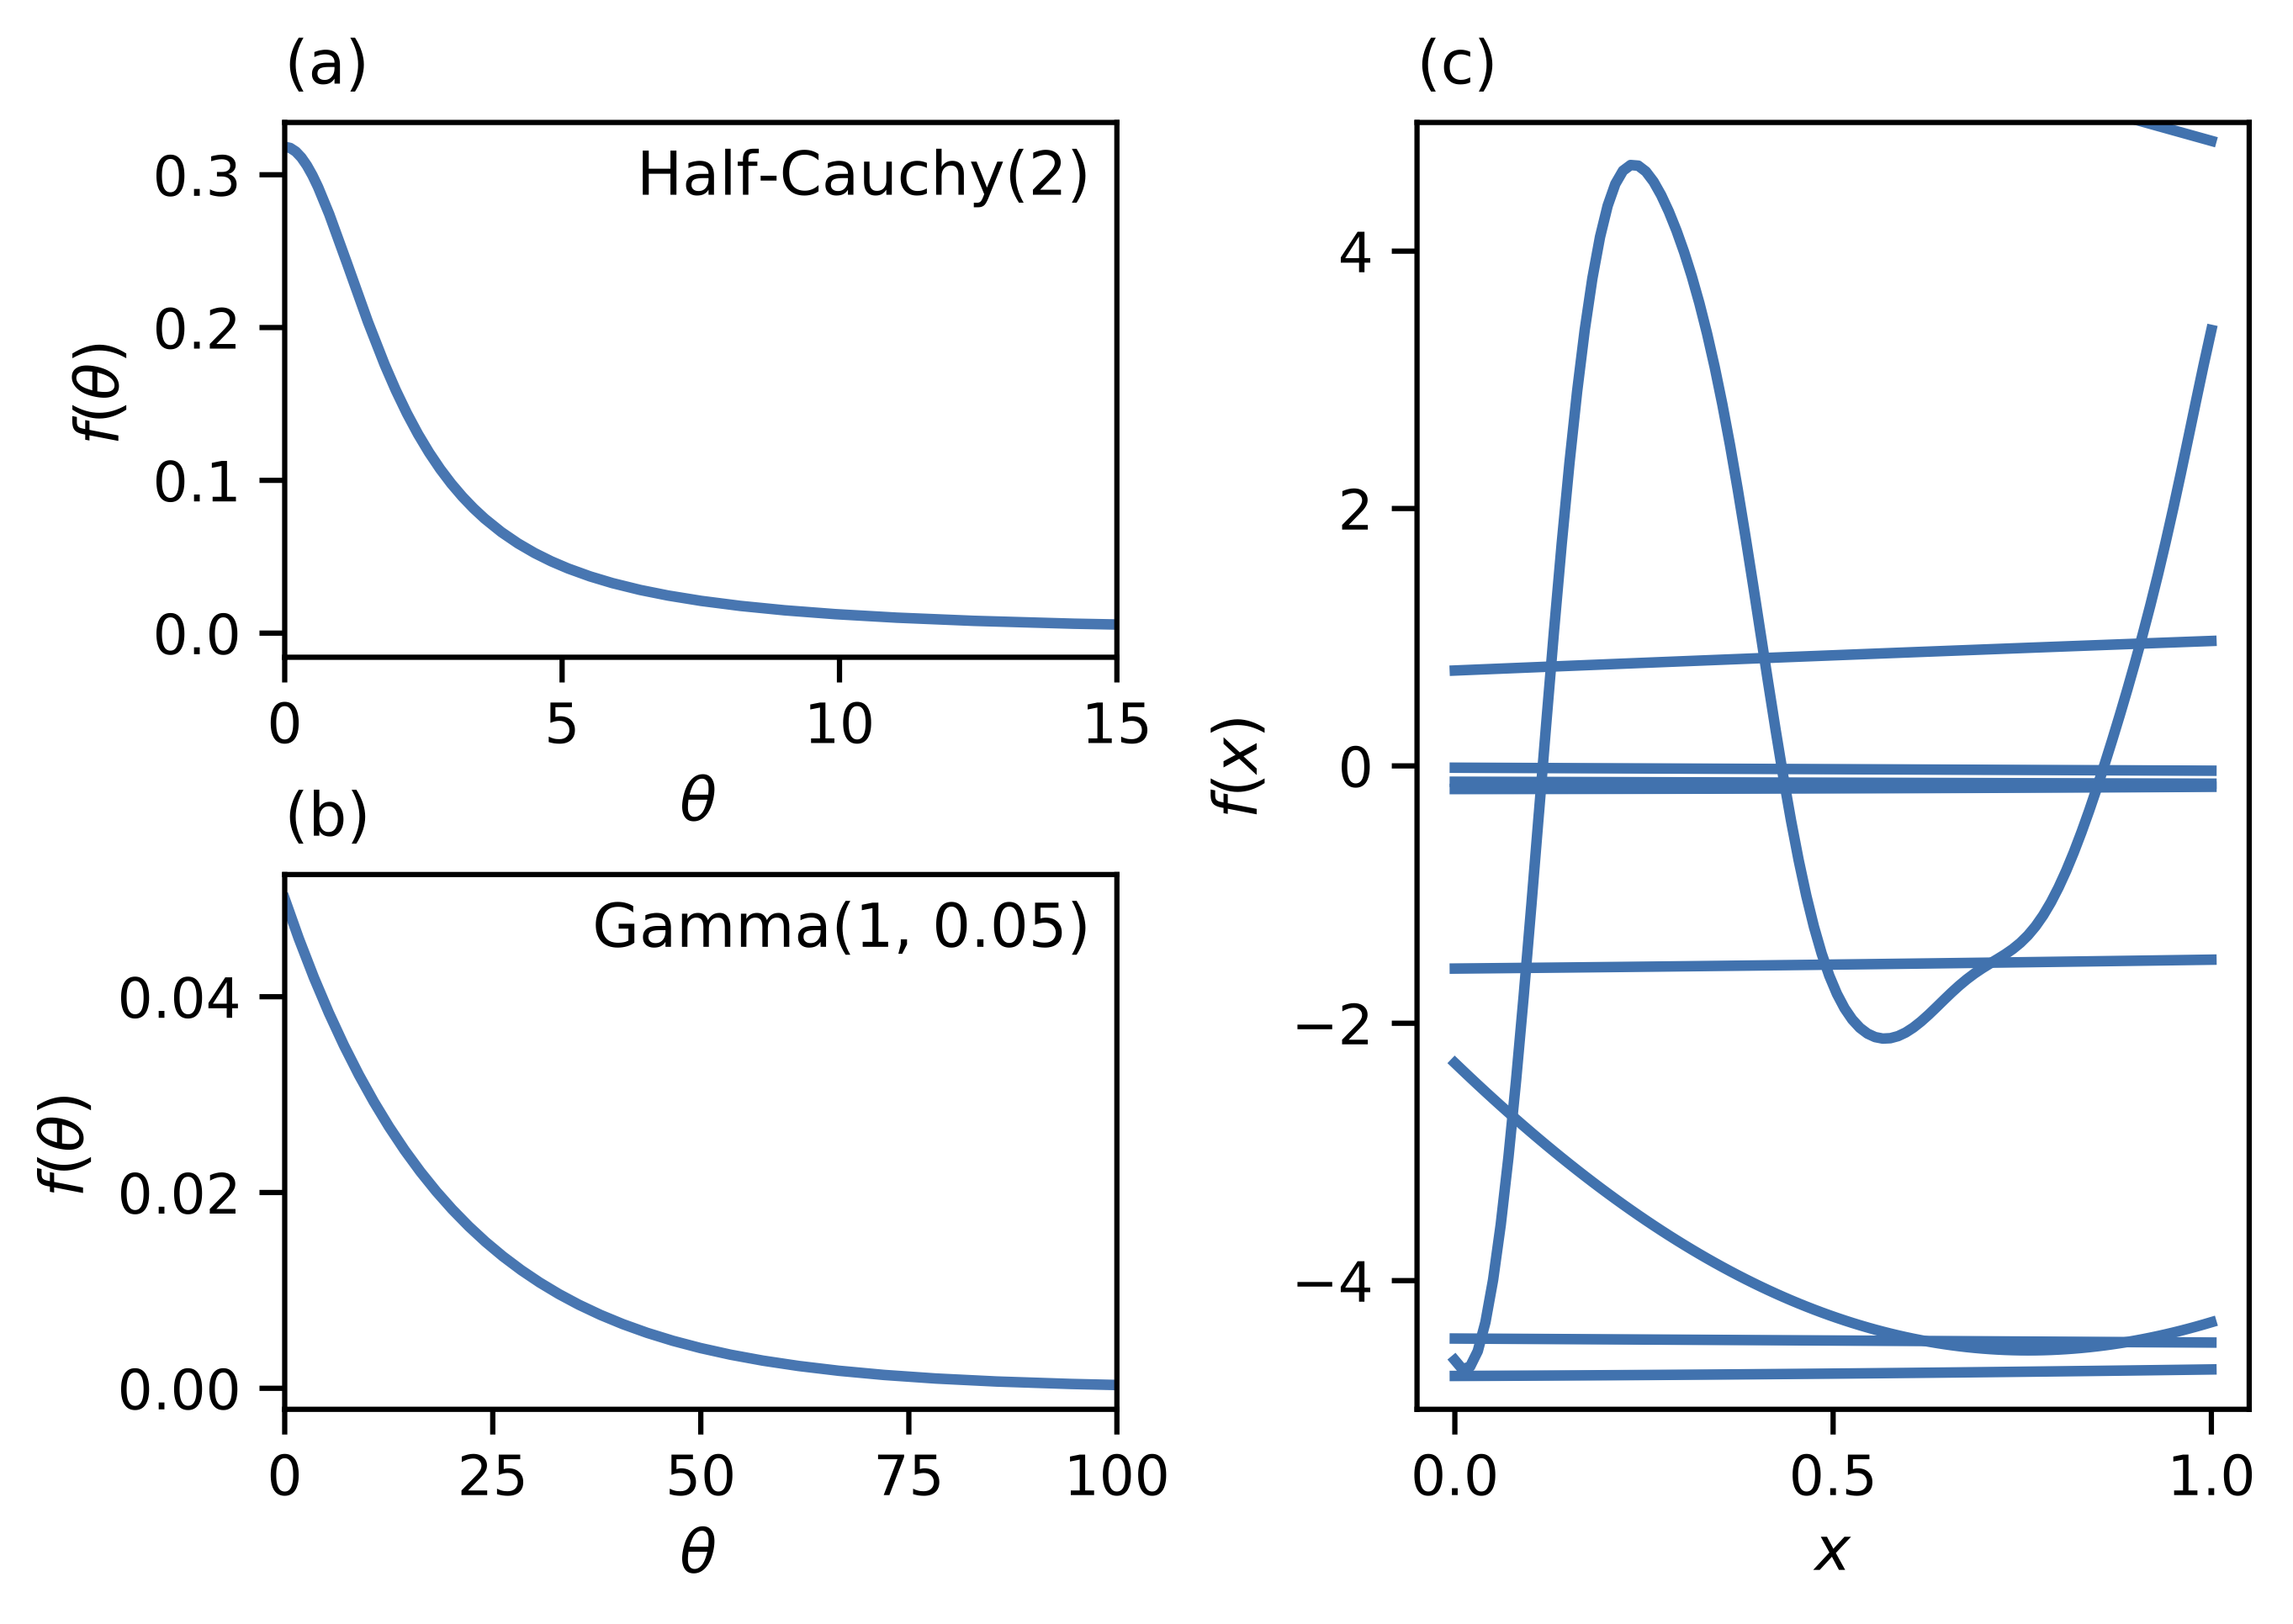
\includegraphics[width=0.8\textwidth]{chapters/msm_optimization/figures/prior_functions.png}
    \label{fig:priors}
\end{figure}

All predictors were scaled to lie in the range $[0, 1]$ to aid interpretation of the kernel length-scale parameters, $l$. Before scaling the integer predictors ($\tau$, $m$ and $n$) two other transformations, $T(\cdot)$, were considered: the identity $I(\cdot)$, and a logarithmic transformation, $\log(\cdot)$. The categorical predictor, $\chi$, was dummy coded \cite{dalyDummyCodingVs2016}, so that a single value $\chi$ is transformed into a $d$ dimensional vector, where $d$ is the number of features in $\chi$.

In order to find the best GPR model for a given response surface, every combination of kernel function and integer predictor transformation was estimated and evaluated using the MAP estimates for the kernel hyper-parameters. This meant that for the response surface of alanine dipeptide with a single integer predictor, $8$ different models were estimated ($4$ different kernels and $2$ predictor transformations). For the response surface of AADH, with three integer predictors, $32$ different models were estimated ($4$ different kernels and $2\times2\times2=8$ different predictor transformations). 

In order to determine the best combination of kernel function and predictor transformation two model selection metrics were used:  mean standardized log loss (MSLL) and the standardized mean square error (SMSE). Each metric was calculated used 10-fold cross validation and any model with $MSLL > 0$ or $SMSE > 1$ was discarded. The remaining models were ranked separately according to MSLL and SMSE ($R_{MSLL}$, $R_{SMSE}$) and ranked according to $\sqrt{R_{MSLL}**2 + R_{SMSE}**2}$. This ranking method was used to ensure a balance between the two selection metrics. 

All data processing was performed using in Python 3.7 using Scikit-learn \cite{pedregosaScikitlearnMachineLearning2011}, Numpy \cite{waltNumPyArrayStructure2011}, Scipy \cite{virtanenSciPyFundamentalAlgorithms2020}, Pandas \cite{mckinneyPandasFoundationalPython2011} and project Jupyter \cite{kluyverJupyterNotebooksPublishing2016}. All GPR calculations were performed in the Python package PyMC3 . 



Model selection from amongst the different kernels was performed by evaluating Mean Standardized Log Loss (MSLL) and Standardized Means Square Error (SMSE) using 10-fold cross-validation. The GPR mean function and kernel parameters were calculated by maximizing the marginal likelihood. 

In order to determine the distribution of the relevance of each hyperparameter a fully Bayesian approach was used. The posterior distributions of kernel parameters were sampled from two independent Markov Chain Monte Carlo chains of $1000$ iterations with $500$ tuning steps using the NUTS [] sampler. Convergence of the sampling was tested using the Gelman-Rubin statistic,$\hat{R}$. All reported models had   $0.99<\hat{R}<1.01$, indicating convergence. 

All charts were produced using the Python packages Matplotlib and Seaborn. Code development was performed in Jupyter notebooks and the PyCharm IDE. 

\subsubsection{Bayesian Optimization}

The expected improvement acquisition function was calculated for each response surface using a grid of 100 points over each continuous/integer valued variables and for each level of each categorical variables. The calculated points of the acquisition function were ranked and the top hyperparameters were scored according to the method in section \ref{sec:msm_fitting}. 



\section{Alanine Dipeptide}


In order understand the process of fitting, understanding and optimising a MSM response surface I first apply this process to the case of Alanine dipeptide (Ala-1), a benchmark system widely used molecular kinetics. There are just two main hyperparameters to adjust for an MSM of alanine dipeptide, the choice of feature $\chi$ and the number of cluster centres, $n$. Previous work on Ala-1 and its two dimensional response surface makes it easy to visualise and to validate the interpretation of the response surface model parameters and the optimisation procedure. This will allow us to have confidence in the this procedure when moving to more complicated example of AADH, with a more complex hyperparameter space and unknown conformational landscape.

\subsection{Response surface}

I sampled the response of an MSM, with $\tau^{MSM}=\SI{9}{\pico\second}$ of Alanine dipeptide with respect to two hyperparameters: $\chi$, the molecule feature, and $n$ the number discrete MSM states. \num{500} values of $\lambda = (\chi, n)$ were sampled, stratified across each value of $\chi$, from the search space described in table \ref{tab:ala2searchspace}. Each MSM was scored using  $\operatorname{VAMP-2}$ on the first $5$ eigenvalues (including the trivial eigenvalue), using \num{20} iterations of 50:50 shuffle-split cross-validation. 

\begin{table}
    \caption{The hyperparameter search space for MSMs of Alanine dipeptide. For each value of the peptide feature, $\chi$, 100 values of $n$ were randomly sampled. Each pair of values $(\chi, n)$ was used to fit and score a MSM.}
    \centering
    \begin{tabularx}{0.9\textwidth}{ |>{\raggedright\arraybackslash}X|l|l| >{\raggedright\arraybackslash}X | } 
    \hline
    \textbf{Hyperparameter} & \textbf{Type} & \textbf{Search space} & \textbf{Details} \\
     \hline\hline
    Feature $\chi$ & Categorical &  $\phi$ torsion &  \\
    & & $\psi$ torsion &  \\ 
    & & $(\phi, \psi)$ torsions &  \\ 
    & & RMSD &  Heavy atoms only\\ 
    & & (x, y, z) coordinates & Heavy atoms only  \\
    \hline 
    Cluster centres, $n$ & Integer & \numlist[list-final-separator = { ... }]{10;20;1000} & Clustered using KMeans-clustering \\
     \hline
    \end{tabularx}
    \label{tab:ala2searchspace}
\end{table}


The average MSM response for each trial are shown in figure \ref{fig:ala1_train_test}.  The test response ($f^{test} = f(\chi, n; x^{test})$, blue points) and the degree of over-fitting ($f^{train} - f^{test}$, orange) are shown as a function of $n$. The  features are ordered according to the  mean of the test response. As expected the  $(\phi, \psi)$ feature has the highest average response. Perhaps unexpectedly, the heavy atom $(x,y,z)$ coordinates feature performs almost as well. 

Each feature shows an almost flat response to increasing $n$ with a similar degree of over-fitting. The flat response can be understood as the interplay of four factors: the eigenfunction discretization error, $\delta$ (see equation xx and fig xxx in [ref prinz]), the dimension of the feature space ($p$, which is $2$ and $30$ for $(\phi, \psi)$ and $(x,y,z)$ coordinates respectively, and $1$ for the remaining features),  the curvature of the slow eigenfunctions, and the large amount of molecular dynamcis data. 

For the $1$ dimensional features, which cannot capture the true slow eigenfunctions, the curvatures of the approximate slow eigenfunctions are small enough that the discretization rapidly falls to a minimum and below other sources of error (sampling error). Even for the large values of $n$, the count matrix is sufficiently well populated to result in a stable eigenvalue spectrum. 

For the higher dimensional features, which can capture the true eigenfunctions varying over each dimension, the discretization error will be the dominant source of error for low values of $n$. 



It is clear from inspection of figure \ref{fig:ala1_train_test} that the most relevant hyperparameter for determining the test response is the feature, $\chi$, while the number of cluster centres,  $n$, is almost irrelevant. This information can be encoded the learned parameters of a Gaussian process regression model which will be of benefit in more complicated systems with more than two hyperparameters. 

In order to fit a GP to this data a number of modelling choices need to be made: 
\begin{enumerate}
    \item the choice of kernel function for determining the covariance of the response,
    \item the transformations of the predictors.  
\end{enumerate}

I have chosen to model the response surface as a stationary Gaussian process, meaning that the covariance between the response is a function of differences in the values of the predictors i.e. 
\begin{equation}
k(\mathbf{\lambda}, \mathbf{\lambda'}) = k(|\mathbf{\lambda} - \mathbf{\lambda'}|)
\end{equation}
The total covariance function is a product of individual these functions over each predictor:
\begin{equation}\label{eqn:kernel_form}
    k(|\mathbf{\lambda}-\mathbf{\lambda}'|; \Theta) = 
    \eta^{2}\prod_i k_{M}(|\lambda_{i}-\lambda_{i}'|; \nu, l_i)
    +\sigma_{n}^{2}\delta_{\lambda, \lambda'}
\end{equation}
where  the product runs over the predictors; $\eta$ controls the total variation in the response function; $\sigma_{n}^{2}$ is the variance due to measurement error; and  $k_{M}(\cdot; \nu, l)$ are kernels in the Mat\'{e}rn class. I consider kernels with $\nu=\sfrac{1}{2},\sfrac{3}{2},\sfrac{5}{2},\infty$. These are alternatively known as an exponential,Mat\'{e}rn 3-2, Mat\'{e}rn 5-2 and the Gaussian kernels. The value of $\nu$ and $l$ together determine the `roughness' of the Gaussian process. 

I chose to transform the predictors in a number of different ways. $\chi$ is an unordered categorical predictor and there can be no distance metric defined between its levels. To overcome this I use one-hot encoding (dummy coding) to transform the $5$ levels of $\chi$ into a $5$d vector of predictors (e.g. $\chi = \phi$ torsions $\rangle (0, 0, 1, 0, 0)$).  For $n$ I considered two possible transformations, $T(n)$: linear/identity transformation $I(n)$ and a log transformation $\log{(n)}$. After applying either one of these transformations, I scaled the predictor to lie in the range $[0, 1]$ in order to make the learned parameters of the covariance function comparable across predictors. 

In order to determine the best combination of kernel function and predictor transformation I calculated the mean standardized log loss (MSLL) and the standardized mean square error (SMSE) using 10-fold cross validation for each combination on a maximum marginal likelihood Gaussian process regression model.  The results of the comparison are shown in Table \ref{tab:ala2_fit_results}. 



The largest improvement in fit, as measured by both the MSLL and SMSE, comes from changing the transformation from $I(n)$ to $\log{(n)}$. This is unsurprising given that the shape of the response for the $(\phi, \psi)$ and $(x,y,z)$ features (panels (a) and (c) in figure \ref{fig:ala1_train_test}) is a clearly non-stationary process: the correlation with respect to changes in $n$ is much lower for $n\leq 100$ than for $n\geq 100$ where the response is flat. The log transformation smooths the response with respect to $n$ and makes the assumption of a stationarity more plausible. The small differences in fit with different kernels is also unsurprising given the the response is largely flat with respect to $n$. The best fitting model, as judged by both the smallest SMSE and MSLL, uses a log transformation of the number of clusters and a Mat{\'e}rn 5-2 kernel. I use these two modelling choices in all further modelling of the Alanine dipeptide response surface.  

The response surface using this parameters and fit on the entire data set is shown in figure \ref{fig:ala1_response}. The blue line shows the mean of the Gaussian process and the shaded blue area represents two standard deviations about the mean value (i.e. the width of the Gaussian process, but ignoring the predicted measurement error, $\sigma_n$). This response surface fits the observed data well, both in terms of the mean response and its uncertainty. The large width of response surface for $n \leq 20$ is a result of transformation of the $n$ into log-space and the comparatively sparse sampling in this region.




% The biggest change in the response surface comes from changing the value of $\chi$: the mean responses of $(\phi, \psi)$ and $(x, y, z)$ for any value of $n$ are above the mean response for the other features. Varying $n$ does have an effect but only for $(\phi, \psi)$ and $(x, y, z)$ features. 

% At low values of $n$ the MSM indicator functions are too large to accurately model the eigenfunctions of the transition matrix, we are in the high bias regime of the `bias-variance' trade-off. As $n$ increases the MSM indicator functions are small enough to accurately capture the change in the transition matrix eigenfunctions, yet large enough to ensure small statistical uncertainty in the transition matrix.  

% For the poorly performing features, the variation of the response with $n$ is flatter - indicating the high bias in the eigenfunctions is dominated by the poor descriptor - the size of the indicator functions is largely irrelevant.  

\begin{figure}
    \centering
    \caption{The response surface for MSMs of alanine dipeptide as a function of the feature, $\chi$ (panels a - e) and number of clusters, $n$ (horizontal axis).  }
    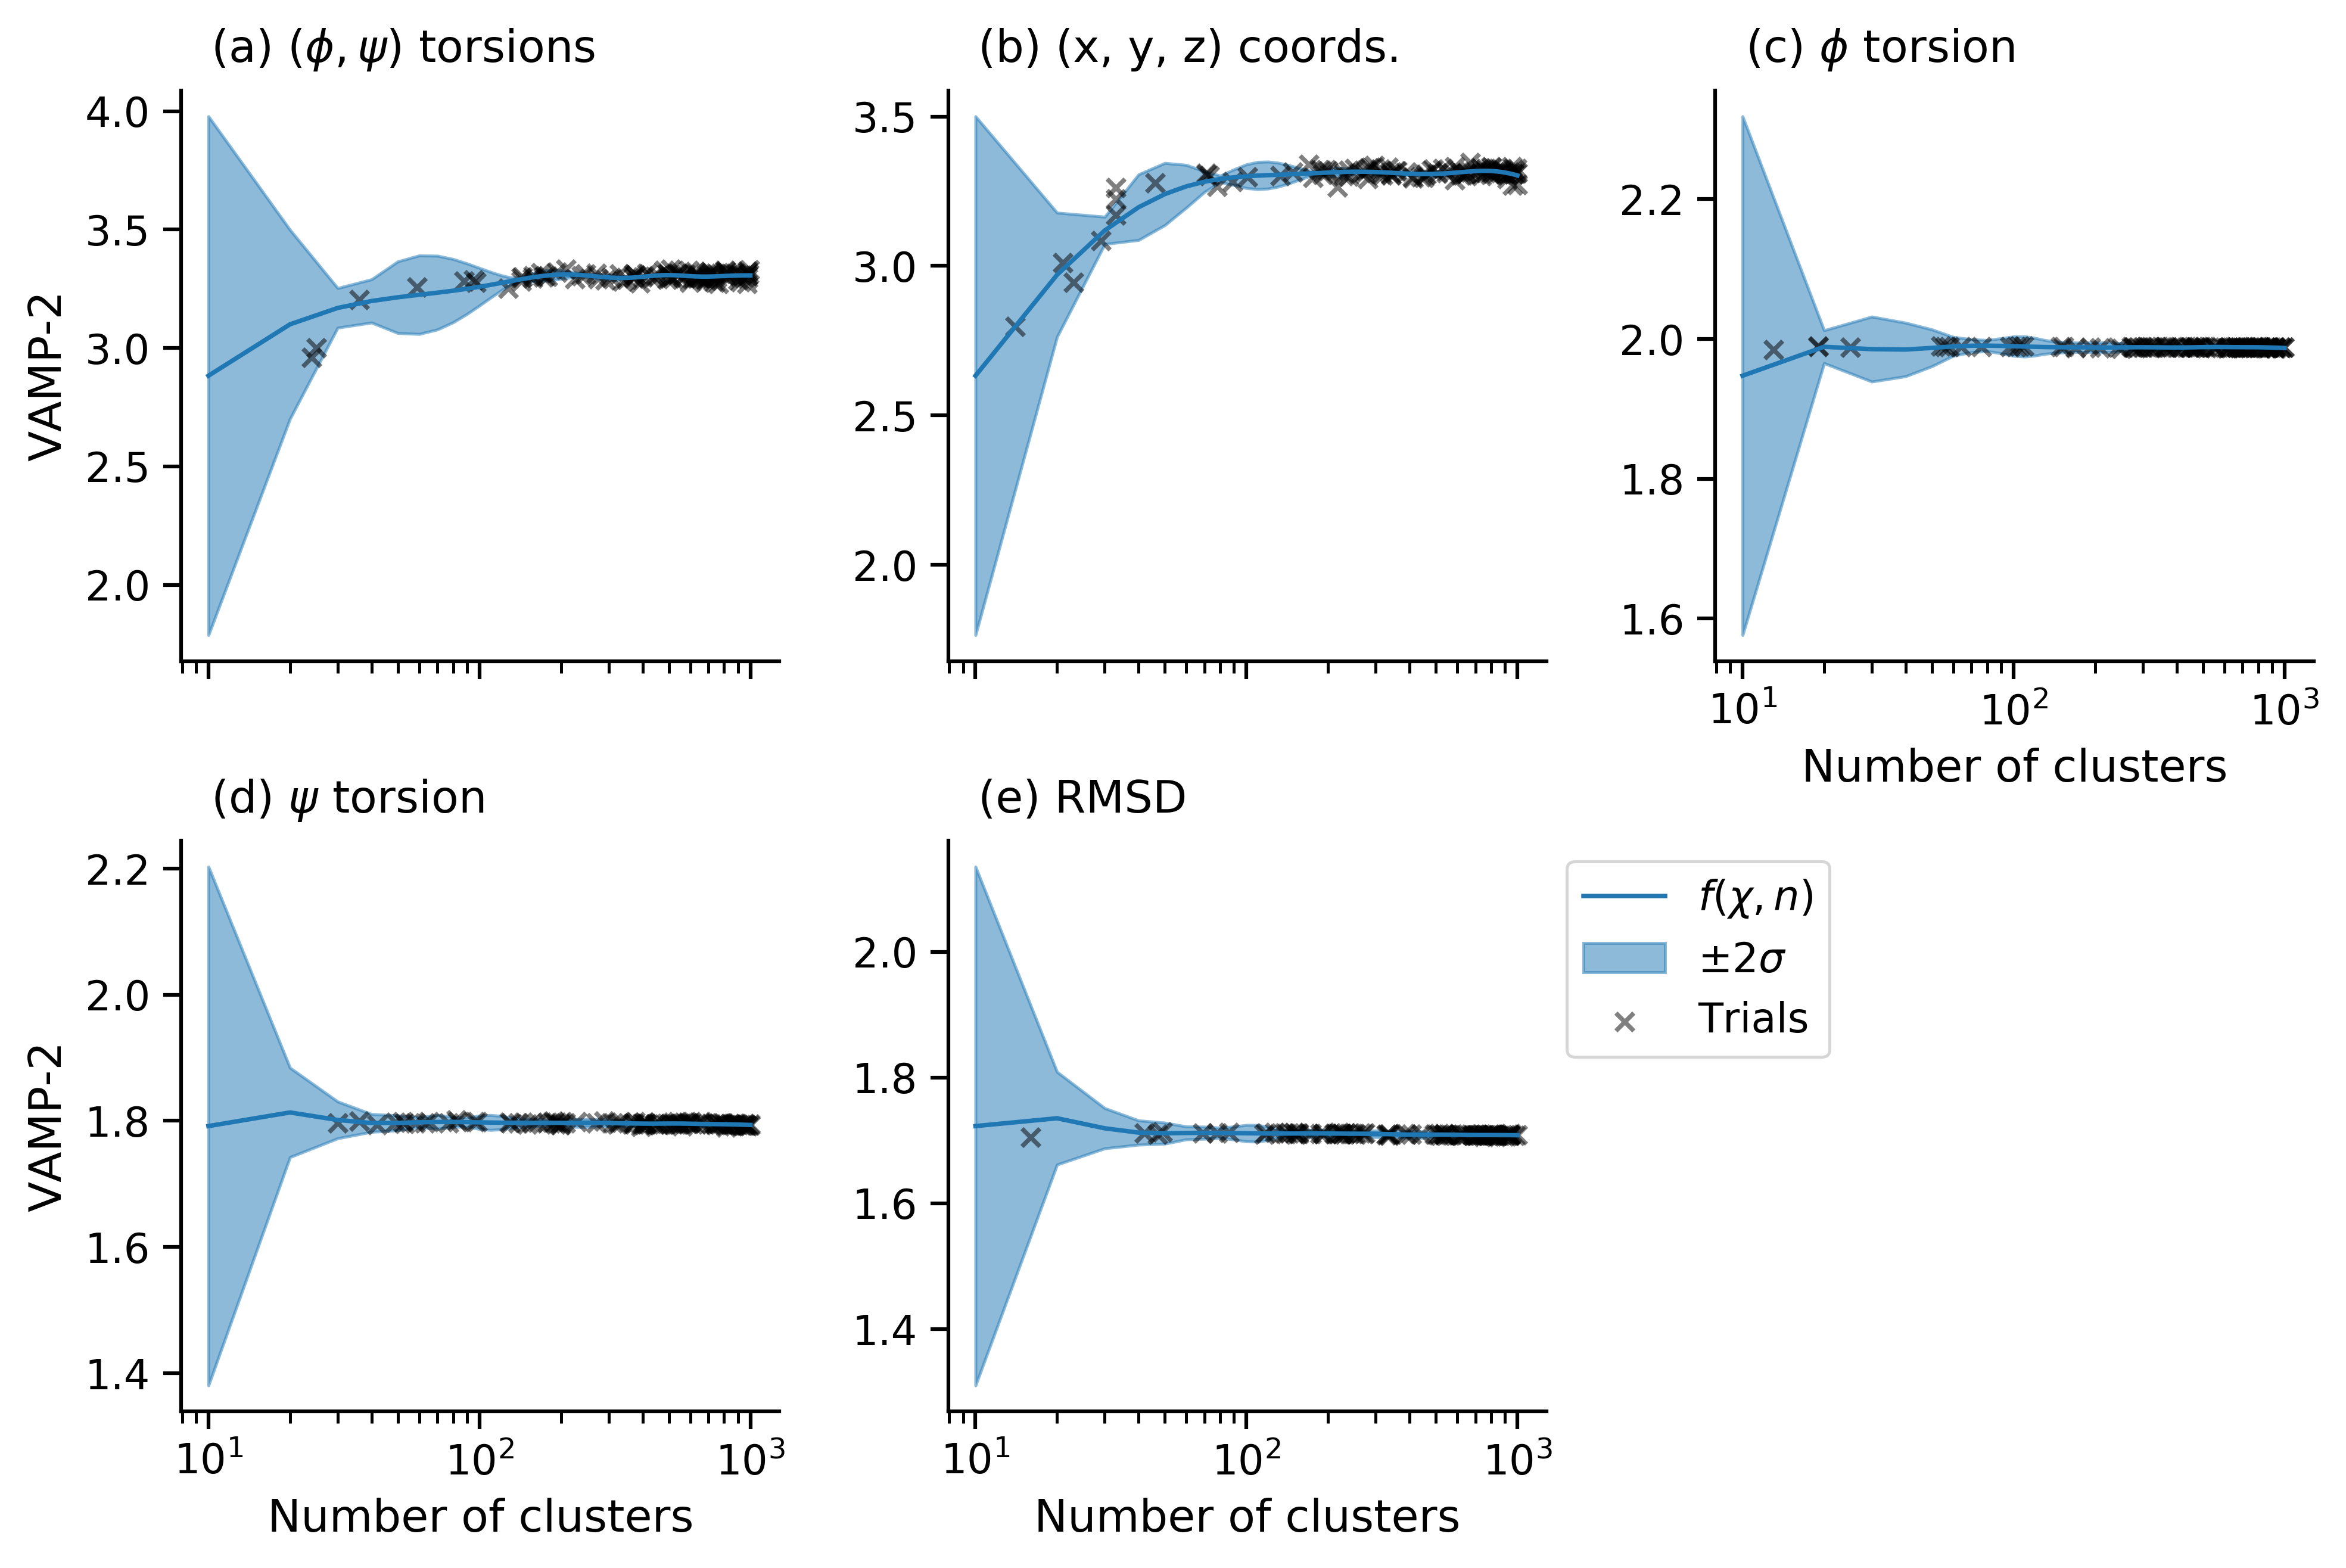
\includegraphics[width=0.8\textwidth]{chapters/msm_optimization/figures/ala1_response_surface.png}
    \label{fig:ala1_response}
\end{figure}

These observations can be quantified and understood by looking at the estimated parameters of the kernel function, $\Theta = (\eta, \sigma_n, l_{\chi[1]}, ..., l_{\chi[5]}, l_{n}) $, where $\chi[1] = 1$ if $\chi = (\phi, \psi)$ torsion, $0$ if not, and similarly for the other levels of $\chi$. The predictor vectors for the response function are given by: $\mathbf{\lambda} = \left(\chi[1],...,\chi[5],n\right)$.

The covariance between $n$ and $n'$ on the same feature, $\chi[1]$, will be a function (see section xxx, equation xxx for the full covariance expression) of the kernel:

\begin{equation}
\begin{split}
    k(\mathbf{\lambda}, \mathbf{\lambda}')& = k\left((1, 0, 0, 0, 0, n), (1, 0, 0, 0, 0, n')\right) \\
    & = \eta^{2}\times 1 \times 1\times 1 \times 1\times 1 \times k_{M}(n, n'; l_{n})
\end{split}
\end{equation}
Here I have dropped the additive noise term $\sigma_{n}$ and the $nu$ parameter for clarity. The learned parameter $l_{n}$ determines the characteristic length scale of the variation of the response with $n$ while on the same feature, $\chi$.

The covariance between $n$ on feature $\chi[1]$ and $n'$ on $\chi[2]$ will be a function of the kernel:

\begin{equation}
\begin{split}
    k(\mathbf{\lambda}, \mathbf{\lambda}')& = k\left((1, 0, 0, 0, 0, n), (0, 1, 0, 0, 0, n')\right) \\
    & = \eta^{2}\times k_{M}\left(1, 0; l_{\chi[1]}\right) \times k_{M}\left(0, 1; l_{\chi[2]}\right) \times 1 \times 1\times 1 \times k_{M}(n, n'; l_{n})
\end{split}
\end{equation}

Then  parameters $l_{\chi}$ therefore determine how much each feature affects the correlation of the other predictors in other features. In other words, and with reference to figure \ref{tab:ala2_fit_results}, the parameters $l_{\chi}$, affect how  the curvature of the mean response in panel (a) affect the curvature in the mean response of panel (b) (and (c) etc.). If both $l_{\chi[1]}$ and $l_{\chi[2]}$ $\gg 1$ then $k_{M} \simeq 1$ then there will be a high degree of correlation between the two responses with respect to $n$. If either of $l_{\chi[1]}$ or $l_{\chi[2]}$ are $\ll 1$ then $k_{M} \simeq 0$ effectively decoupling the response with respect to $n$ in both features. The parameter $\eta$ is simply the baseline correlation between points on the response surface, as well as affecting the width of the response surface.  

This interpretation is behind the definition of the parameter relevance $R = \sfrac{1}{l}$. Box-plots of the posterior relevance for each hyperparameter (calculated using Bayesian estimation) is shown in figure \ref{fig:ala1_relevance}.   

For non-categorical variables low relevance implies different values of $n$ will result in only small changes in the response. The predictor  $\log{(n)}$, has the lowest median relevance of $0.03$. So when choosing a set of hyperparameters it matters less what specific value is chosen. In practical terms this means fewer points in the sample space of $n$ can be chosen without missing potentially important regions. 

For categorical predictors the interpretation of relevance is slightly different. Each level of the predictor (in our case, feature) has a separate value of relevance. High relevance means this level of the predictor  decouples of the response of the model to the other predictors. The relatively high relevance of the $(x,y,z)$ and $(\phi, \psi)$ features means the response does with these features does not influence the response on other features. In practical terms this means including this level in the search space means that you have to search more fully the other predictors. Alternatively, information regarding the shape of the response surface is not shared across levels. 

\begin{figure}
    \centering
    \caption{The relevance of hyperparameters for MSMs of alanine dipeptide. }
    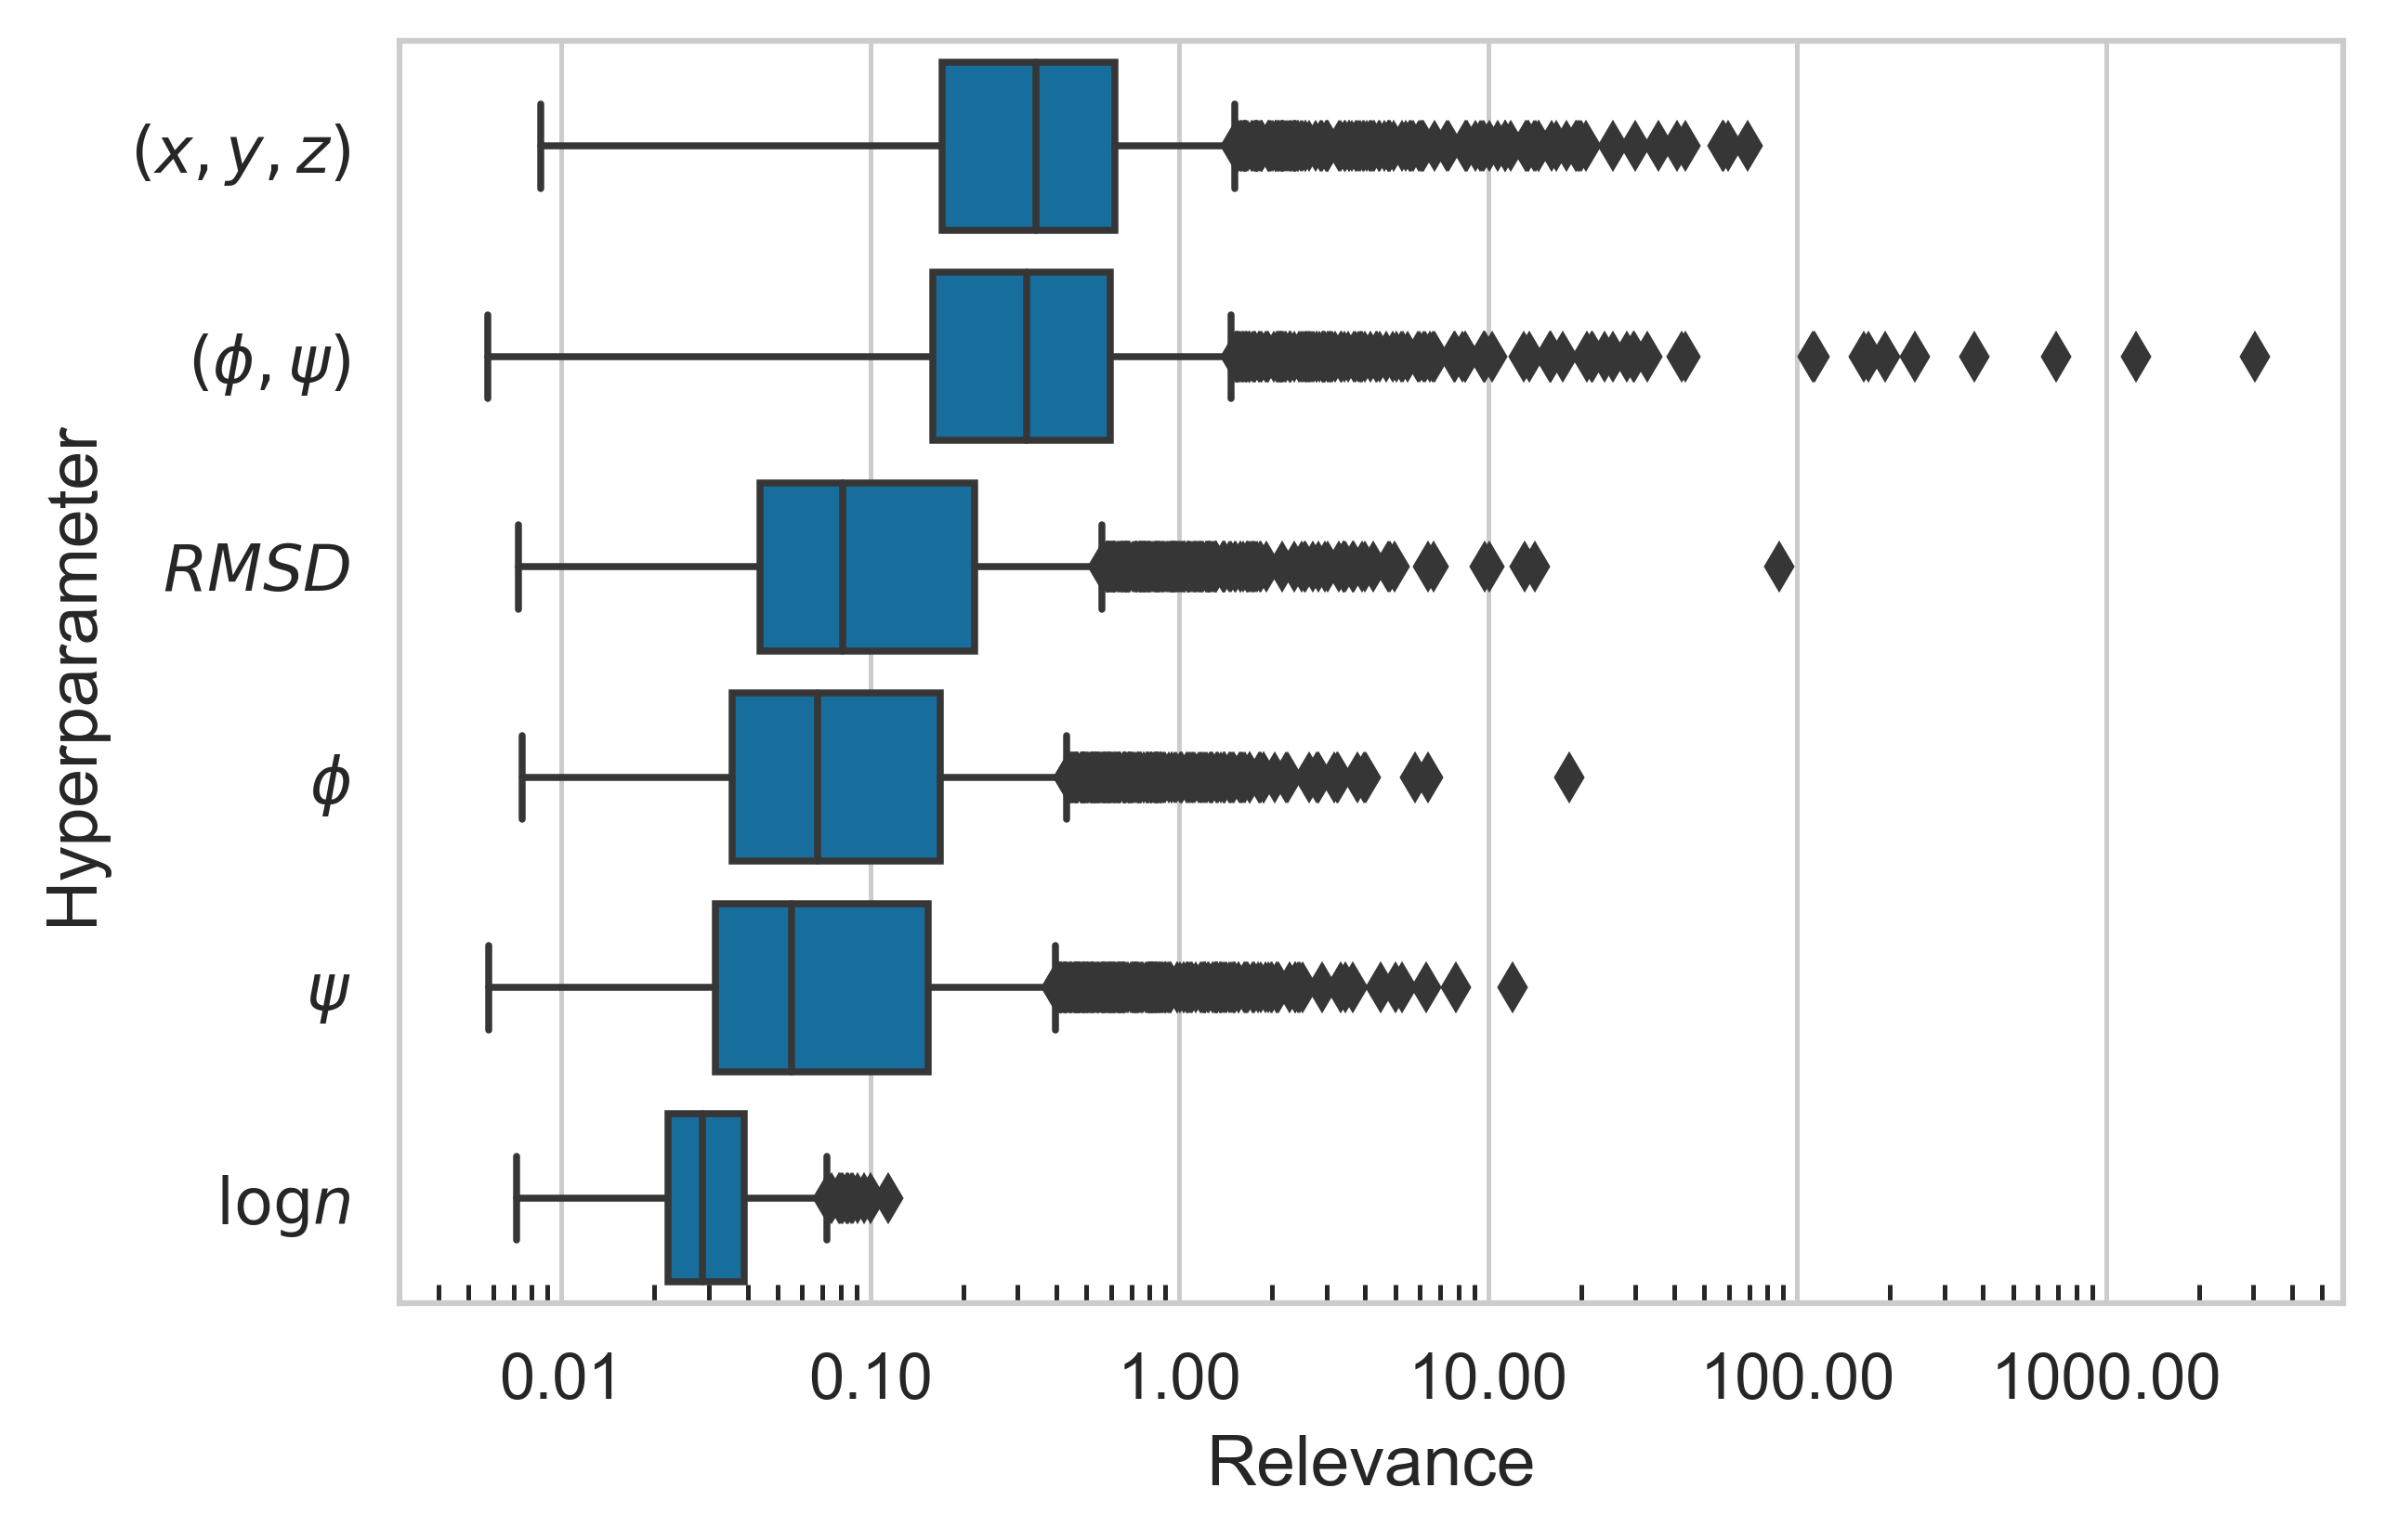
\includegraphics[width=0.8\textwidth]{chapters/msm_optimization/figures/ala1_relevance.png}
    \label{fig:ala1_relevance}
\end{figure}


\subsubsection{Optimization}

The maximum of the response surface \emph{at the trial values} gives the optimum hyperparameters incorporating uncertainty and making full use of all the trial information. For alanine dipeptide the optimum hyperparameters are shown in table xxx. These are the best performing values for which we are most certain.  Given the large amount of sampling required to reach these values, a natural question to ask is: ``could we have arrived at these values with less sampling through optimization''?

In order to answer this question I use Bayesian optimisation to optimise the hyperparameters over the same search space. The BO algorithm must be seeded with a set of trials to build the initial response surface. I chose to seed the algorithm with $30$ and $50$ observations sampled from the $500$ observations previously described (corresponding to $15$ and $25$ observations per predictor). I ran the BO algorithm for $10$ steps and repeated this whole process $5$ times. 


The results of this process are shown in figure xx. The horizontal axes denotes the number of observations used to calculate the response surface and the step of the optimization process. 

\begin{figure}
    \centering
    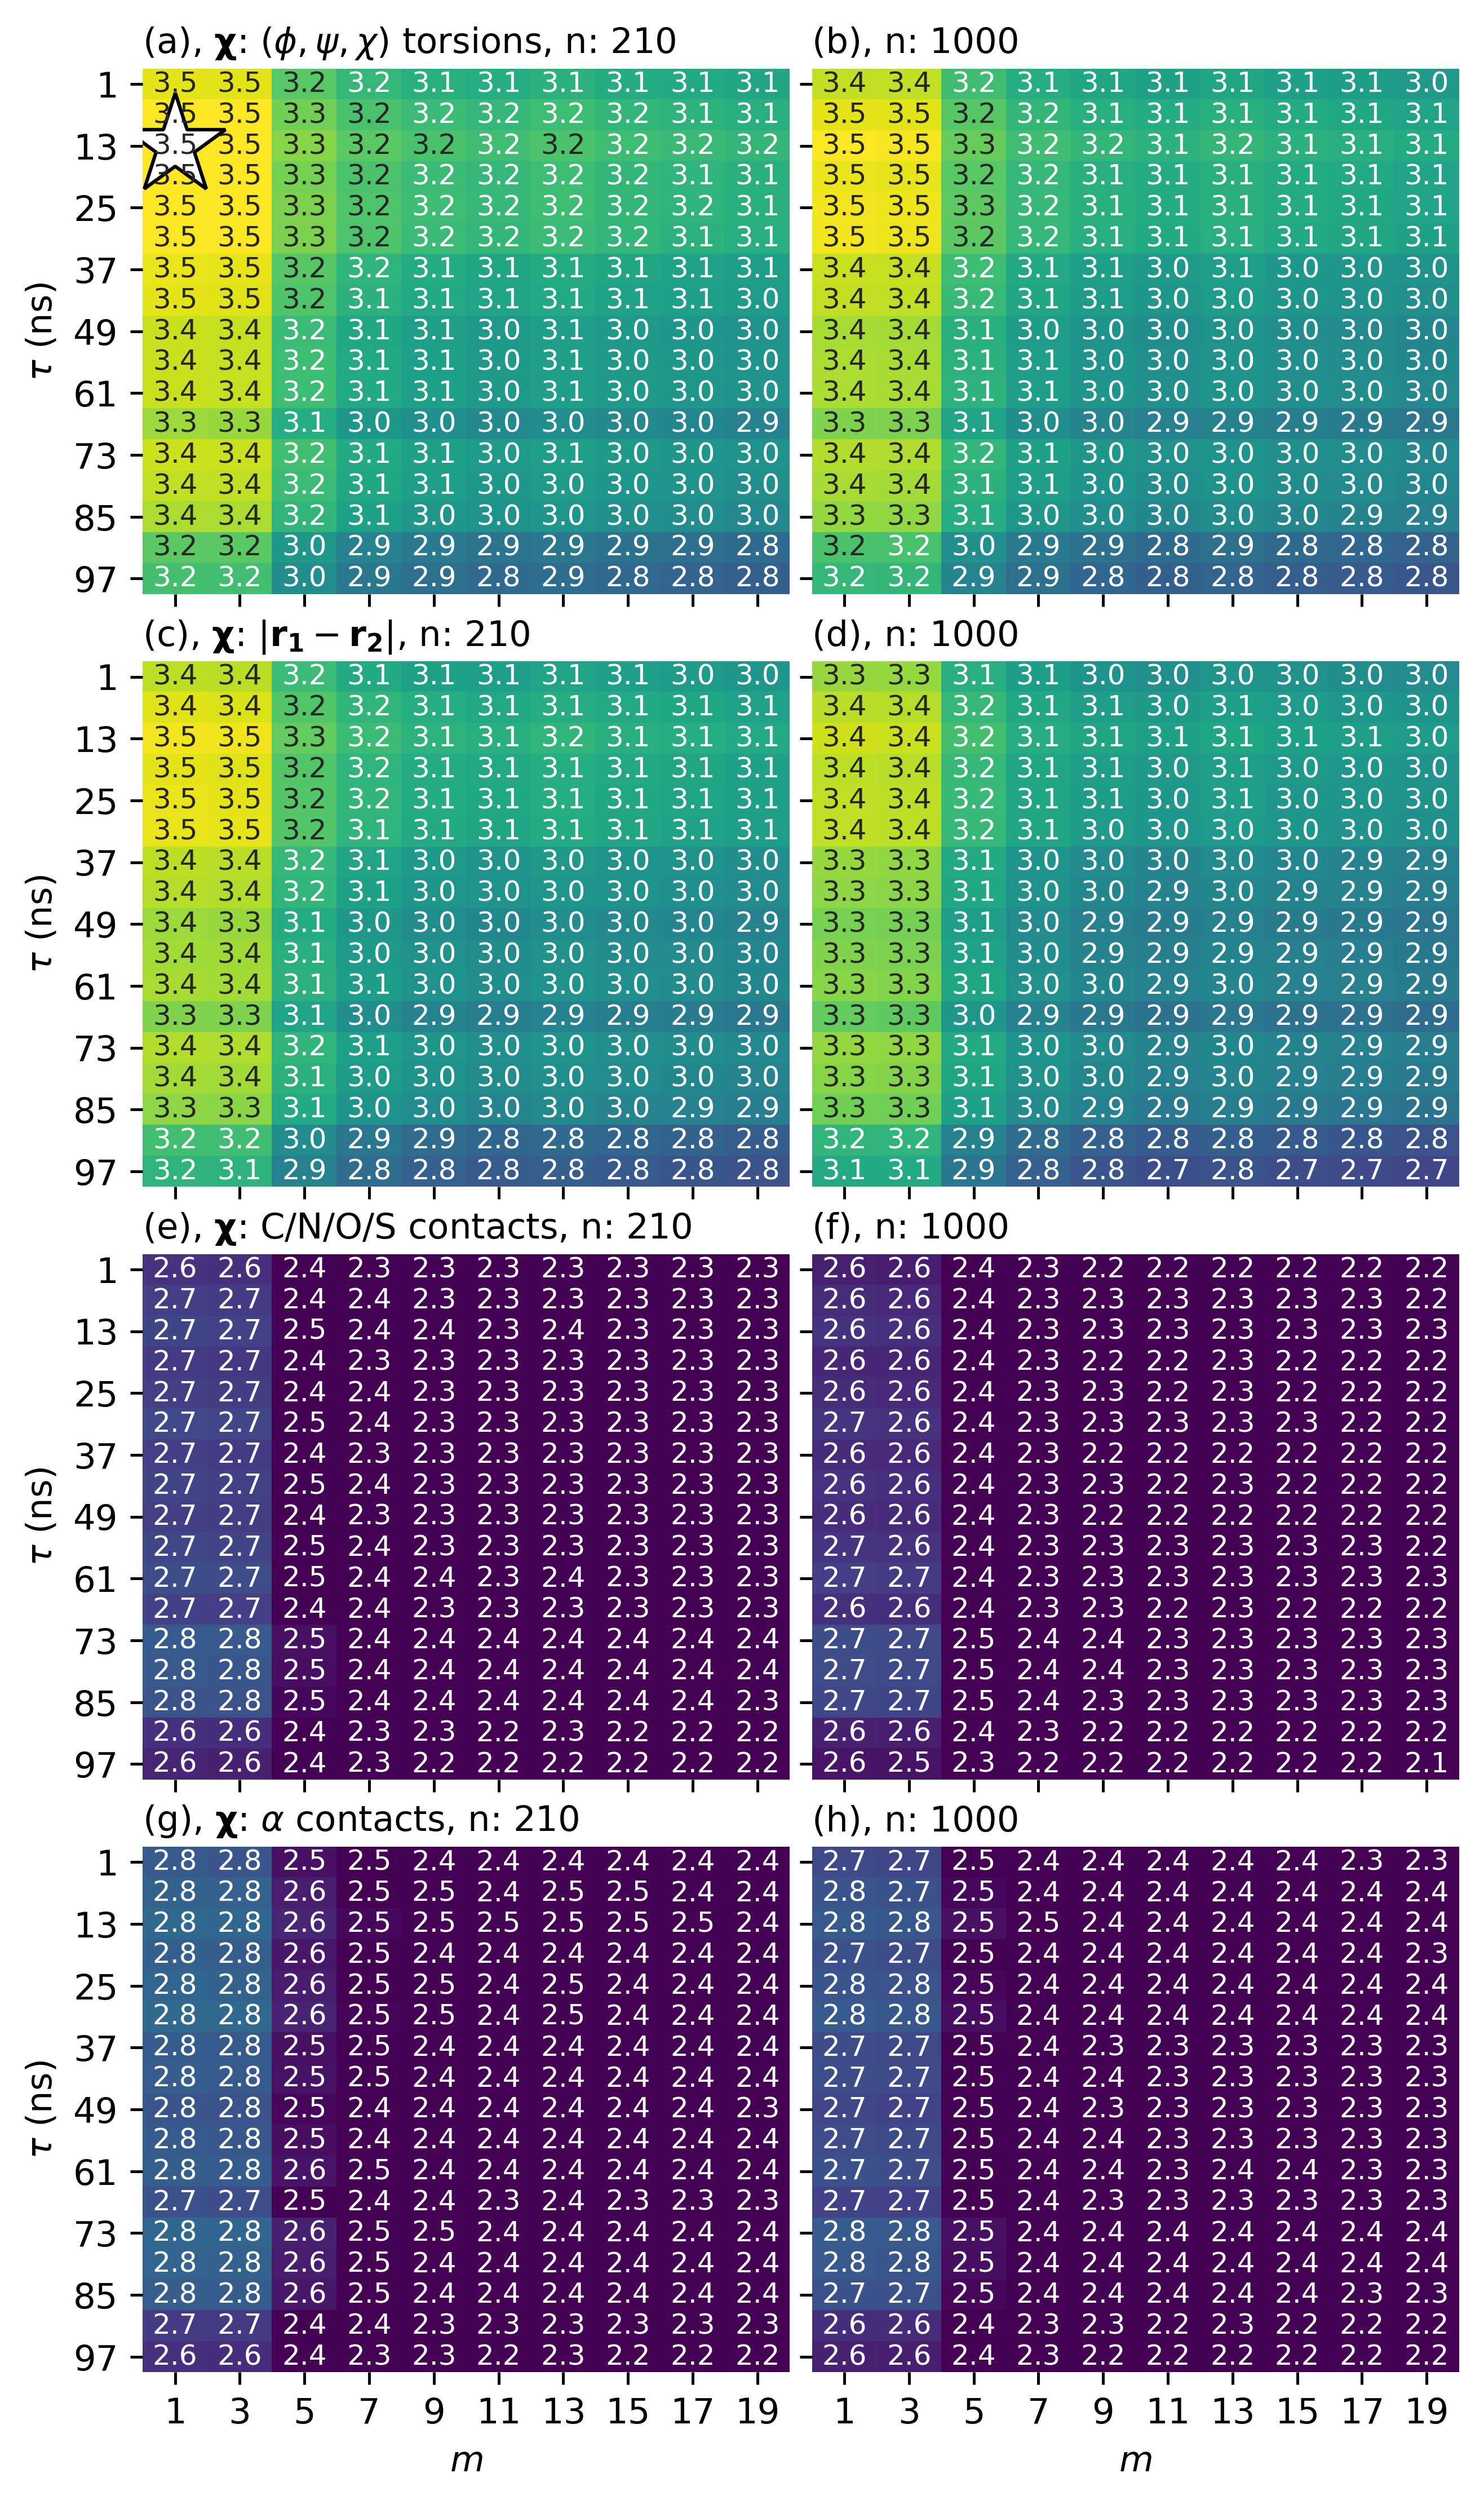
\includegraphics[width=0.8\textwidth]{chapters/msm_optimization/figures/aadh_response_surface_d.png}
    \caption{Caption}
    \label{fig:asdafadf}
\end{figure}

\begin{figure}
    \centering
    \caption{Bayesian optimisation trajectories}
    \subtop[30 trails]{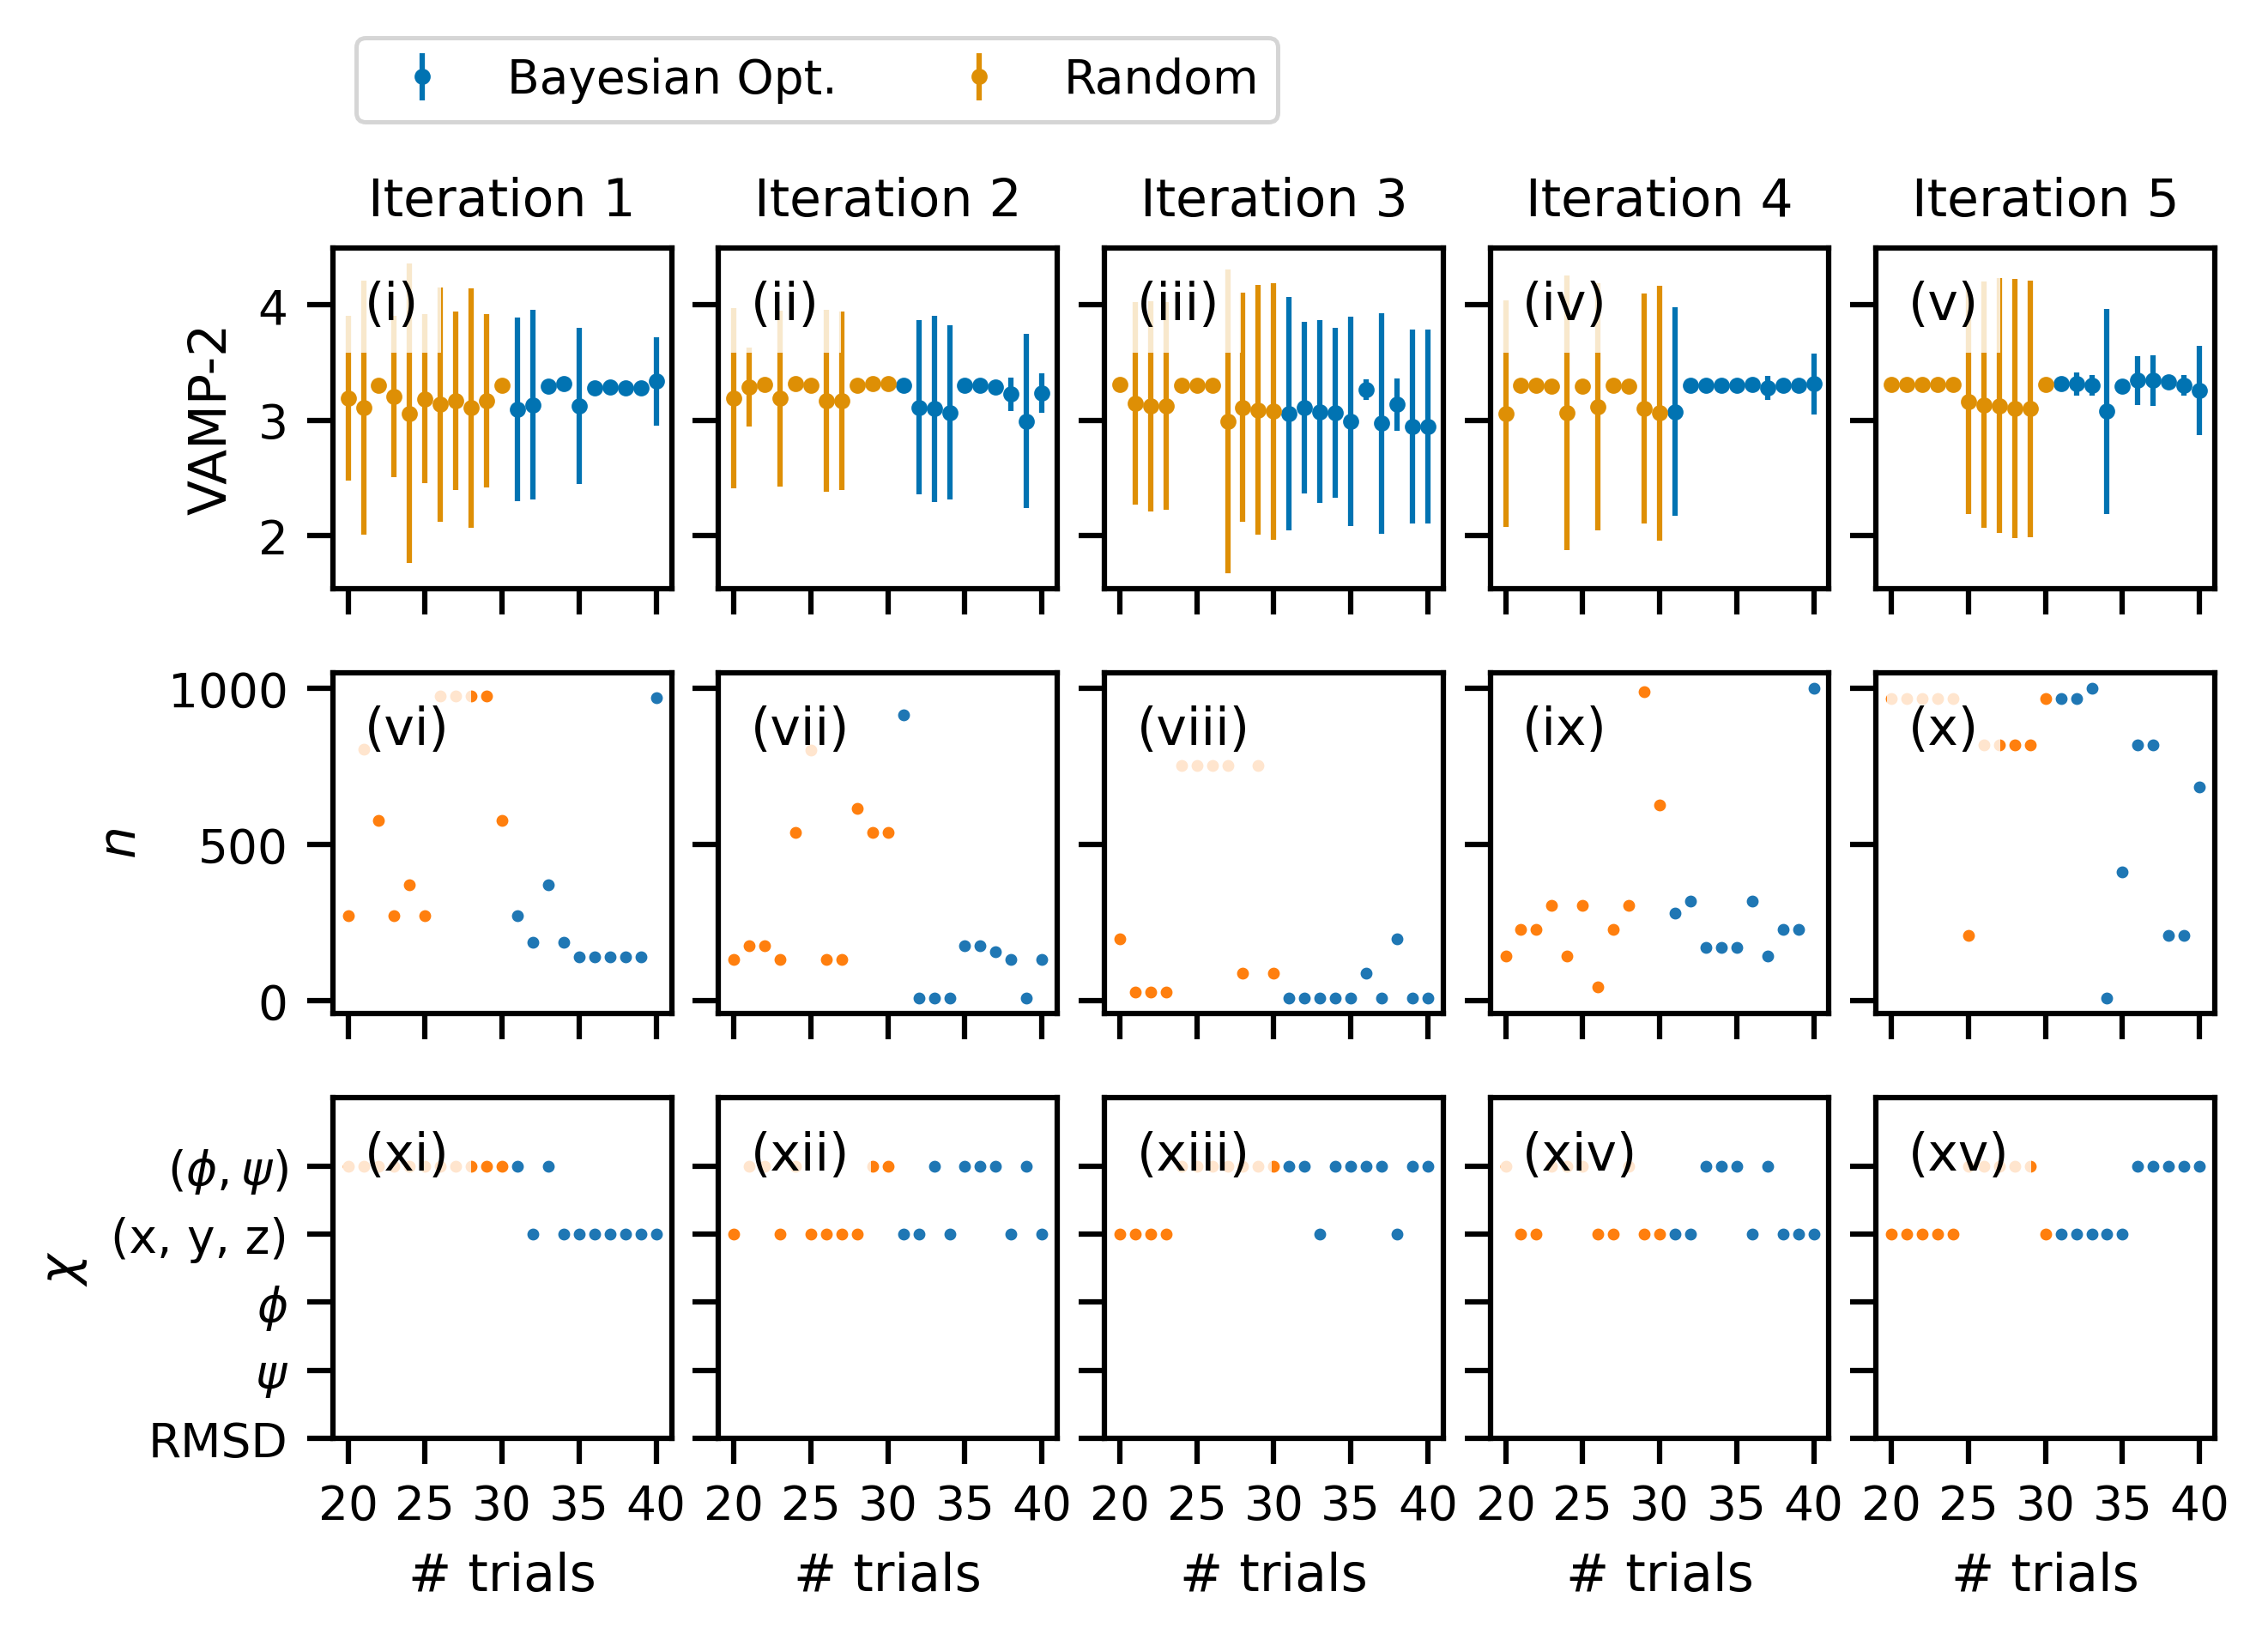
\includegraphics[width=0.9\linewidth]{chapters/msm_optimization/figures/ala1_opt_traj_start_obs_30.png}}
    
    \subtop[50 trials]{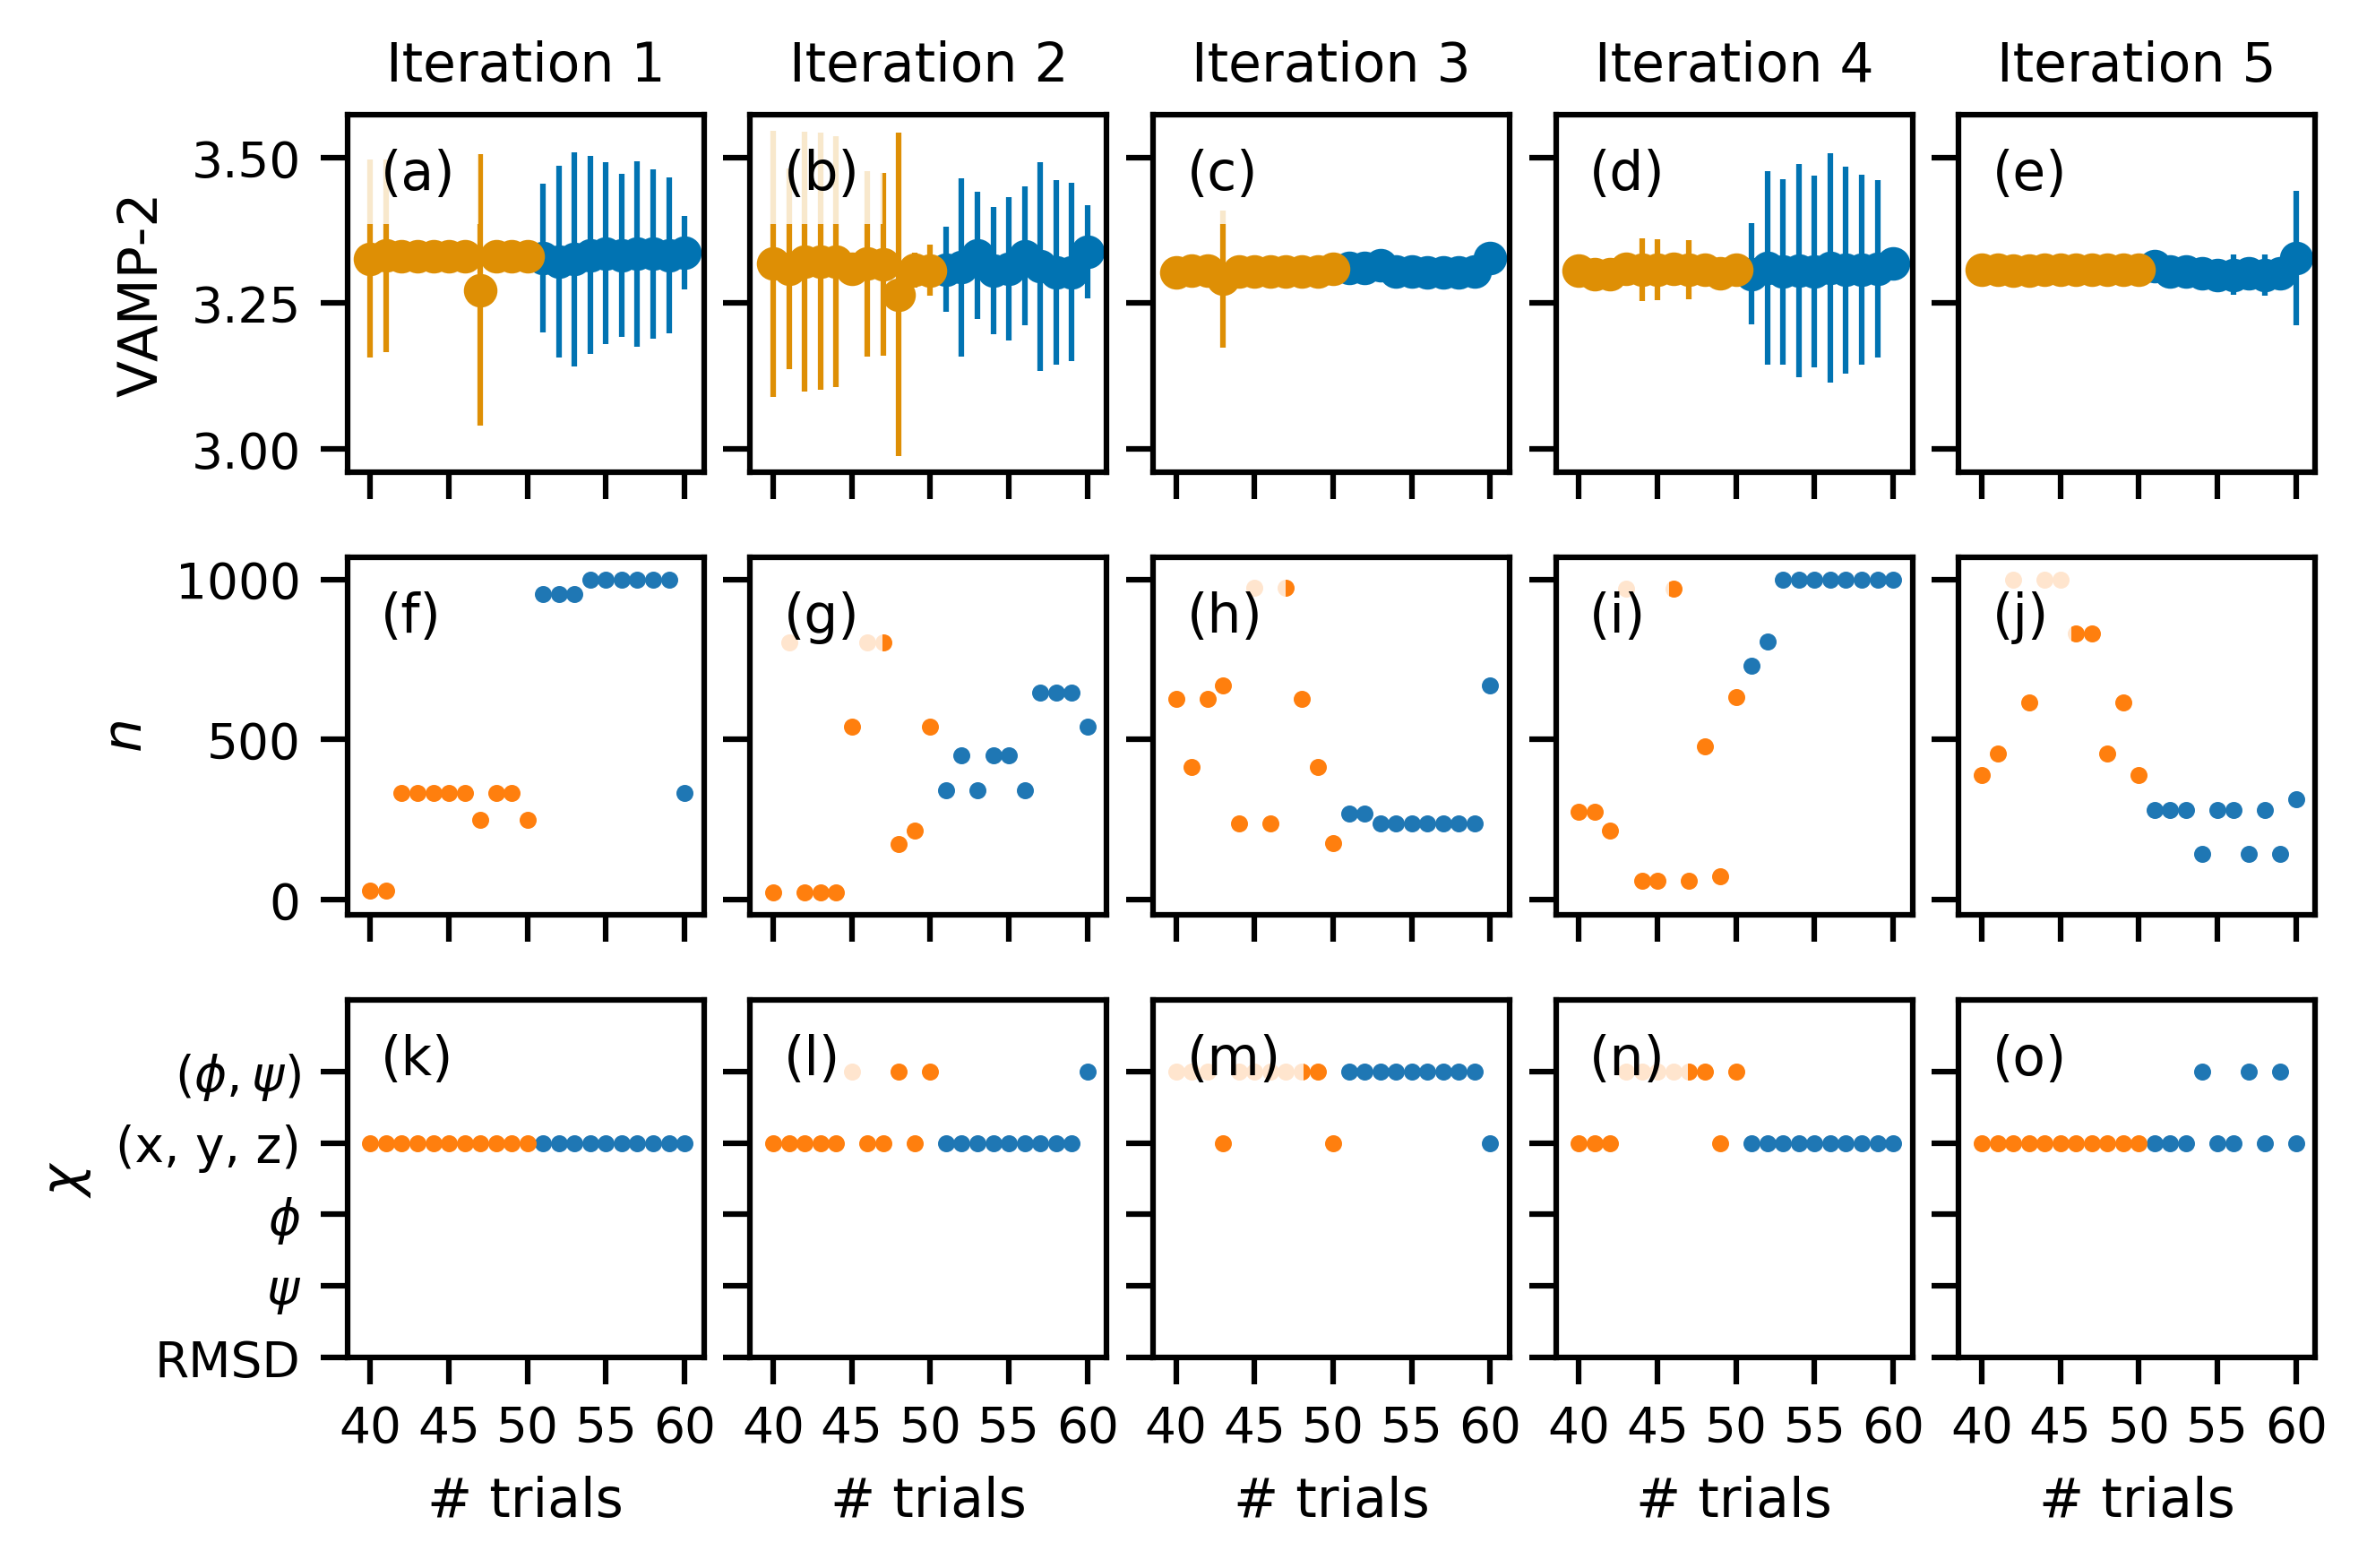
\includegraphics[width=0.9\linewidth]{chapters/msm_optimization/figures/ala1_opt_traj_start_obs_50.png}}
    \label{fig:ala_opt_traj_50}
\end{figure}

\begin{figure}
    \centering
    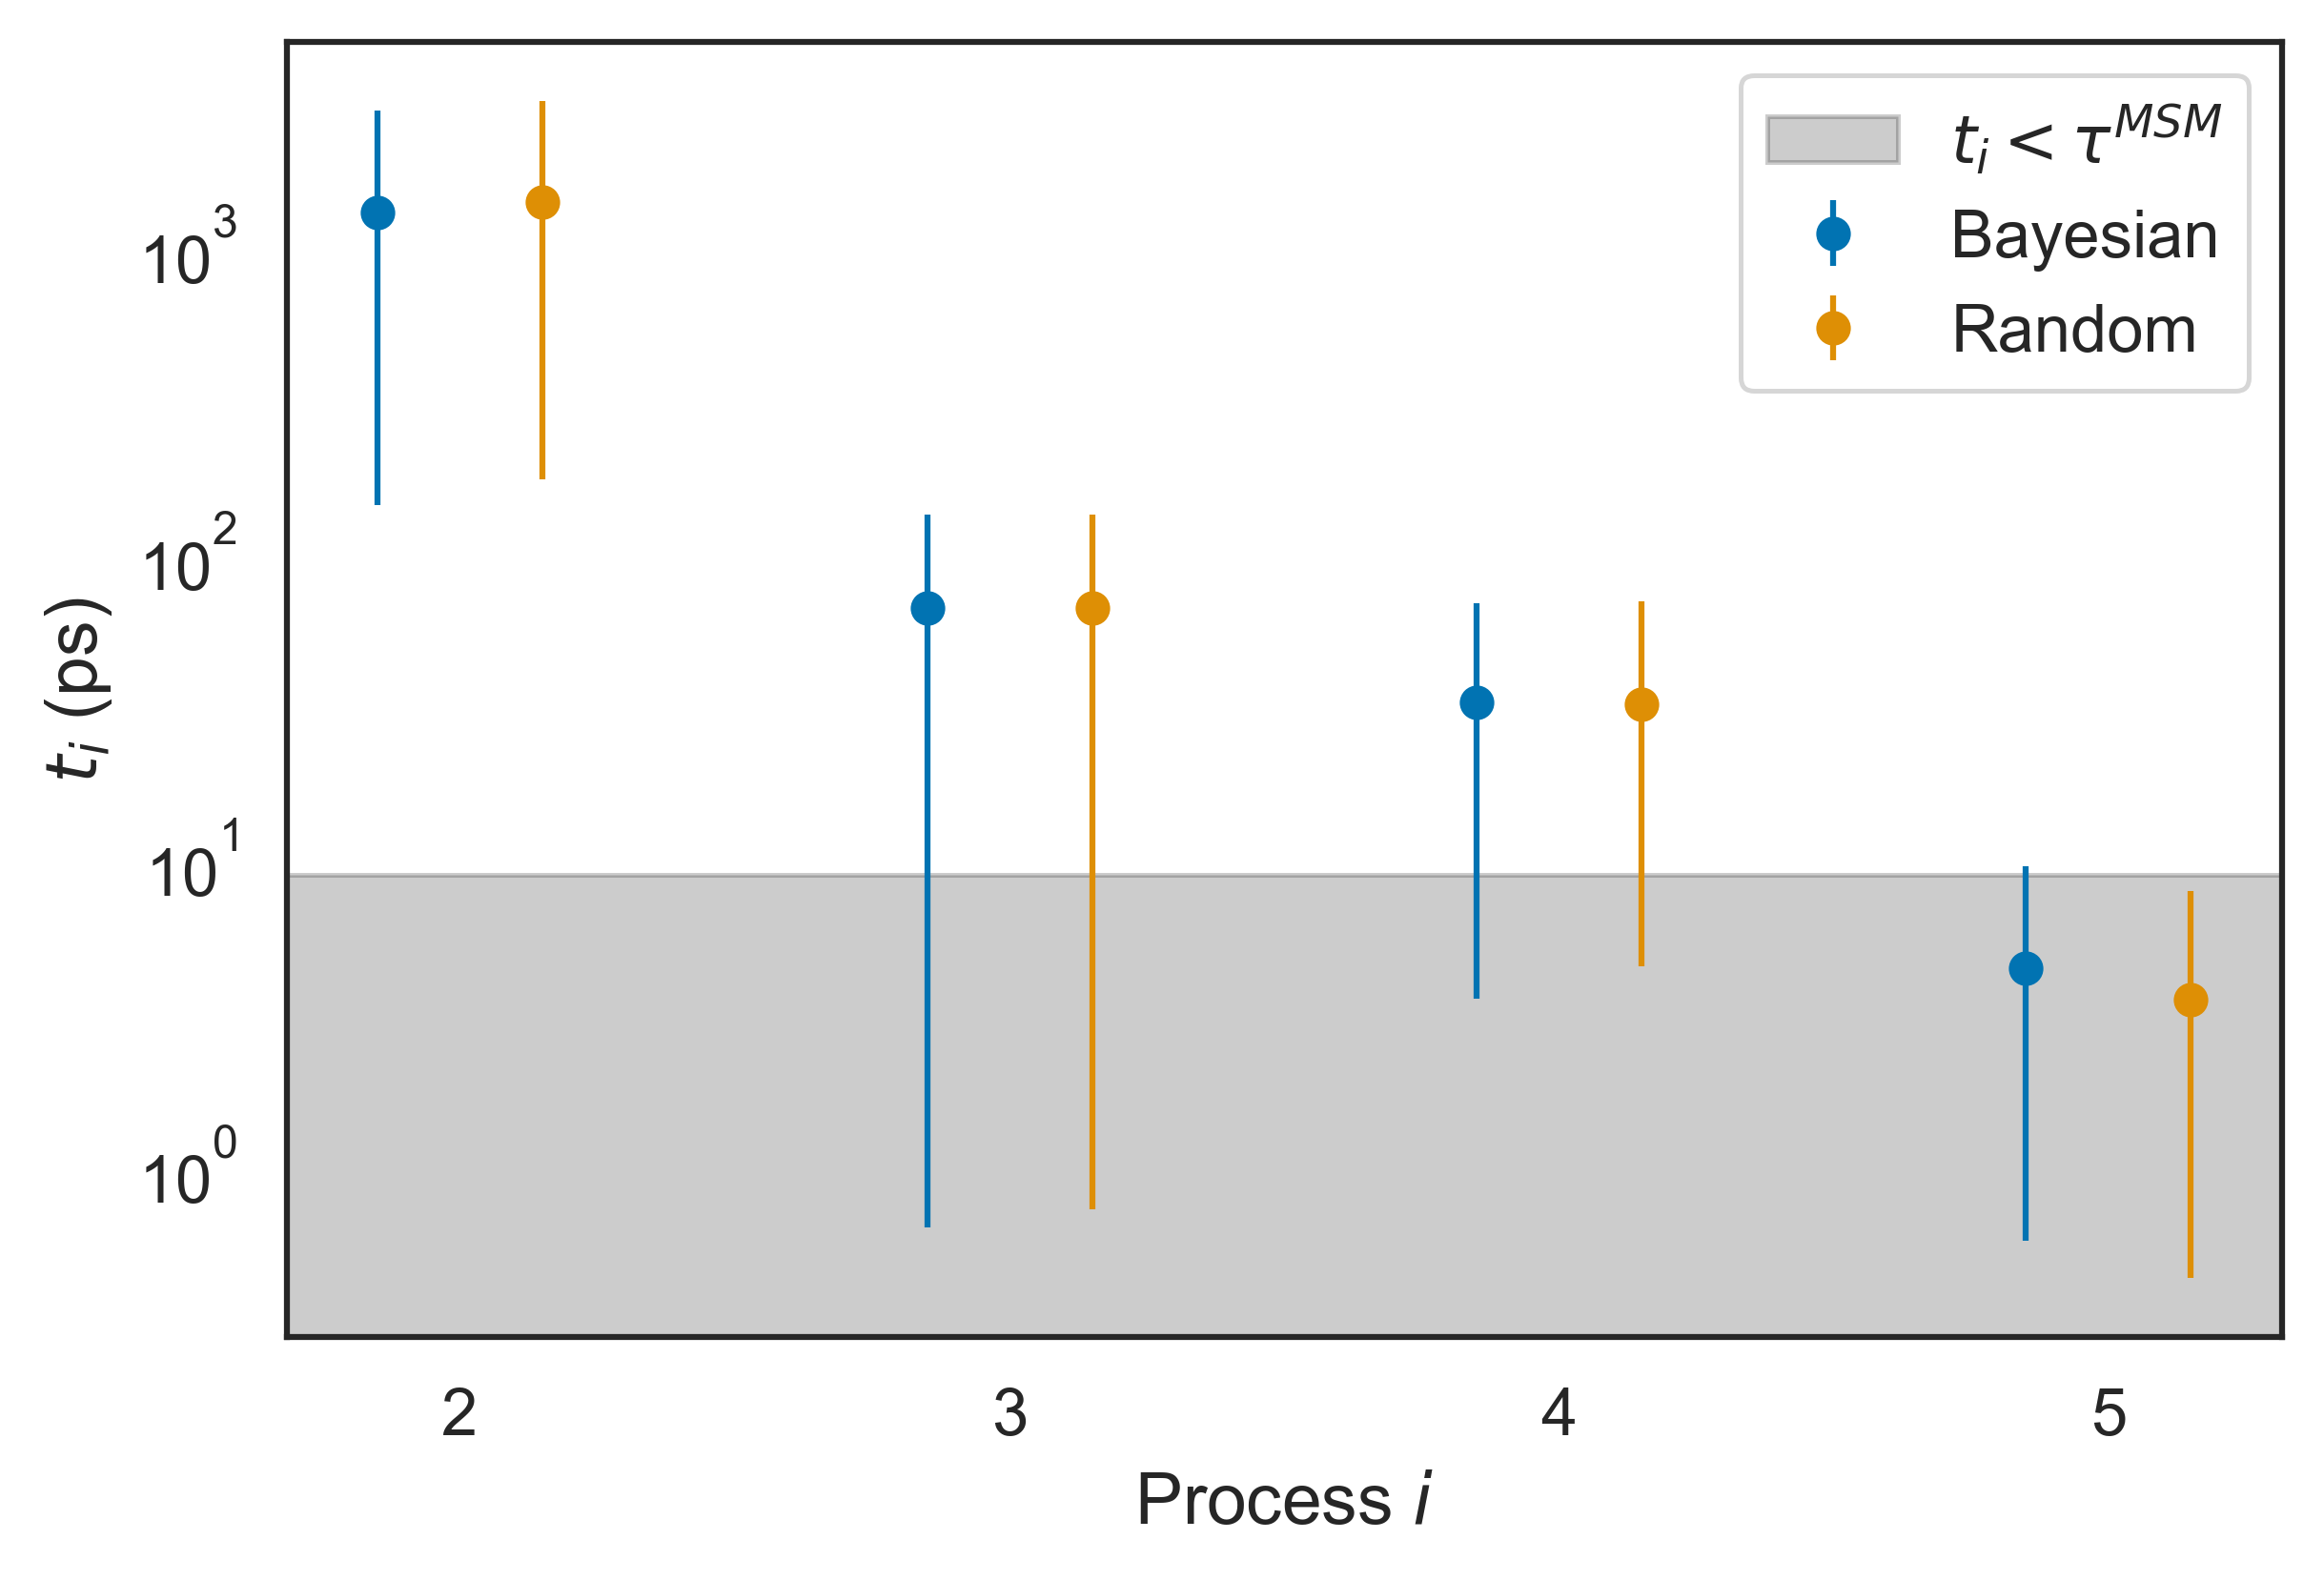
\includegraphics[width=0.8\linewidth]{chapters/msm_optimization/figures/ala1_opt_comparison.png}
    \caption{Caption}
    \label{fig:ala1_best_msm_ts}
\end{figure}
% \begin{figure}
%     \centering
%     \begin{subfigure}[b]{0.3\textwidth}
%         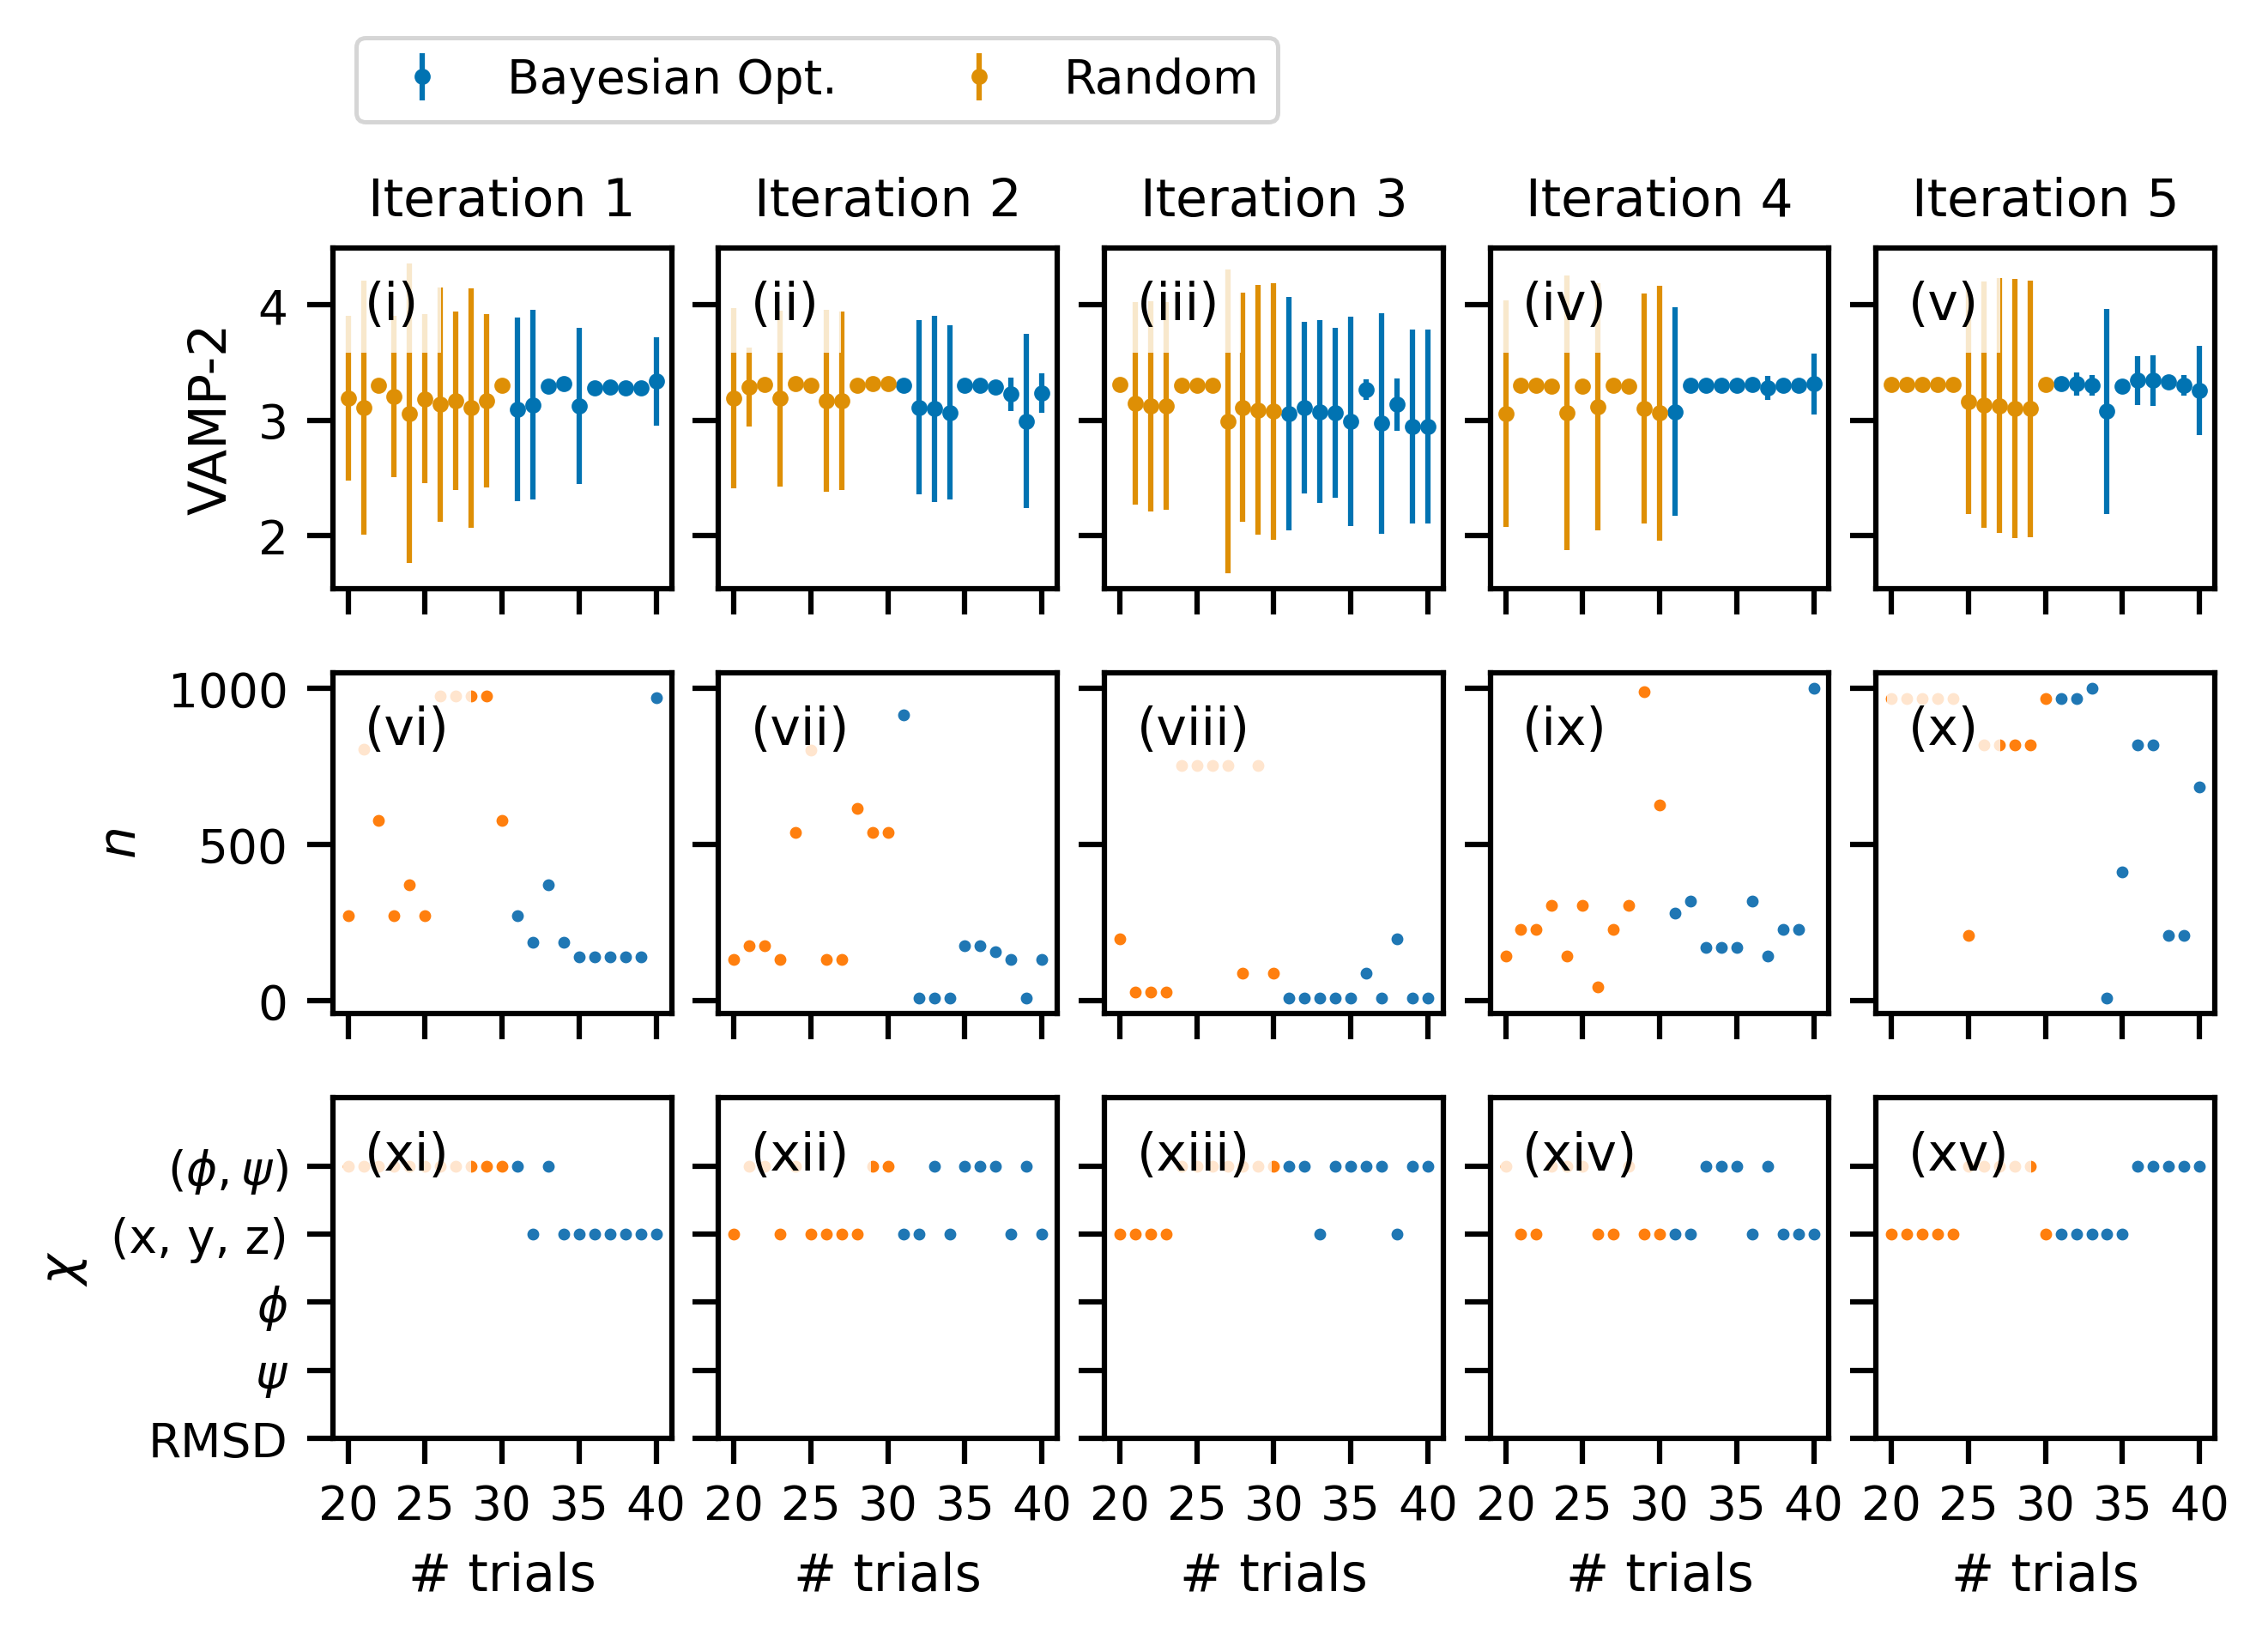
\includegraphics[width=\textwidth]{chapters/msm_optimization/figures/ala1_opt_traj_start_obs_30.png}
%         \caption{A gull}
%         \label{fig:gull}
%     \end{subfigure}
%     ~ %add desired spacing between images, e. g. ~, \quad, \qquad, \hfill etc. 
%       %(or a blank line to force the subfigure onto a new line)
%     \begin{subfigure}[b]{0.3\textwidth}
%         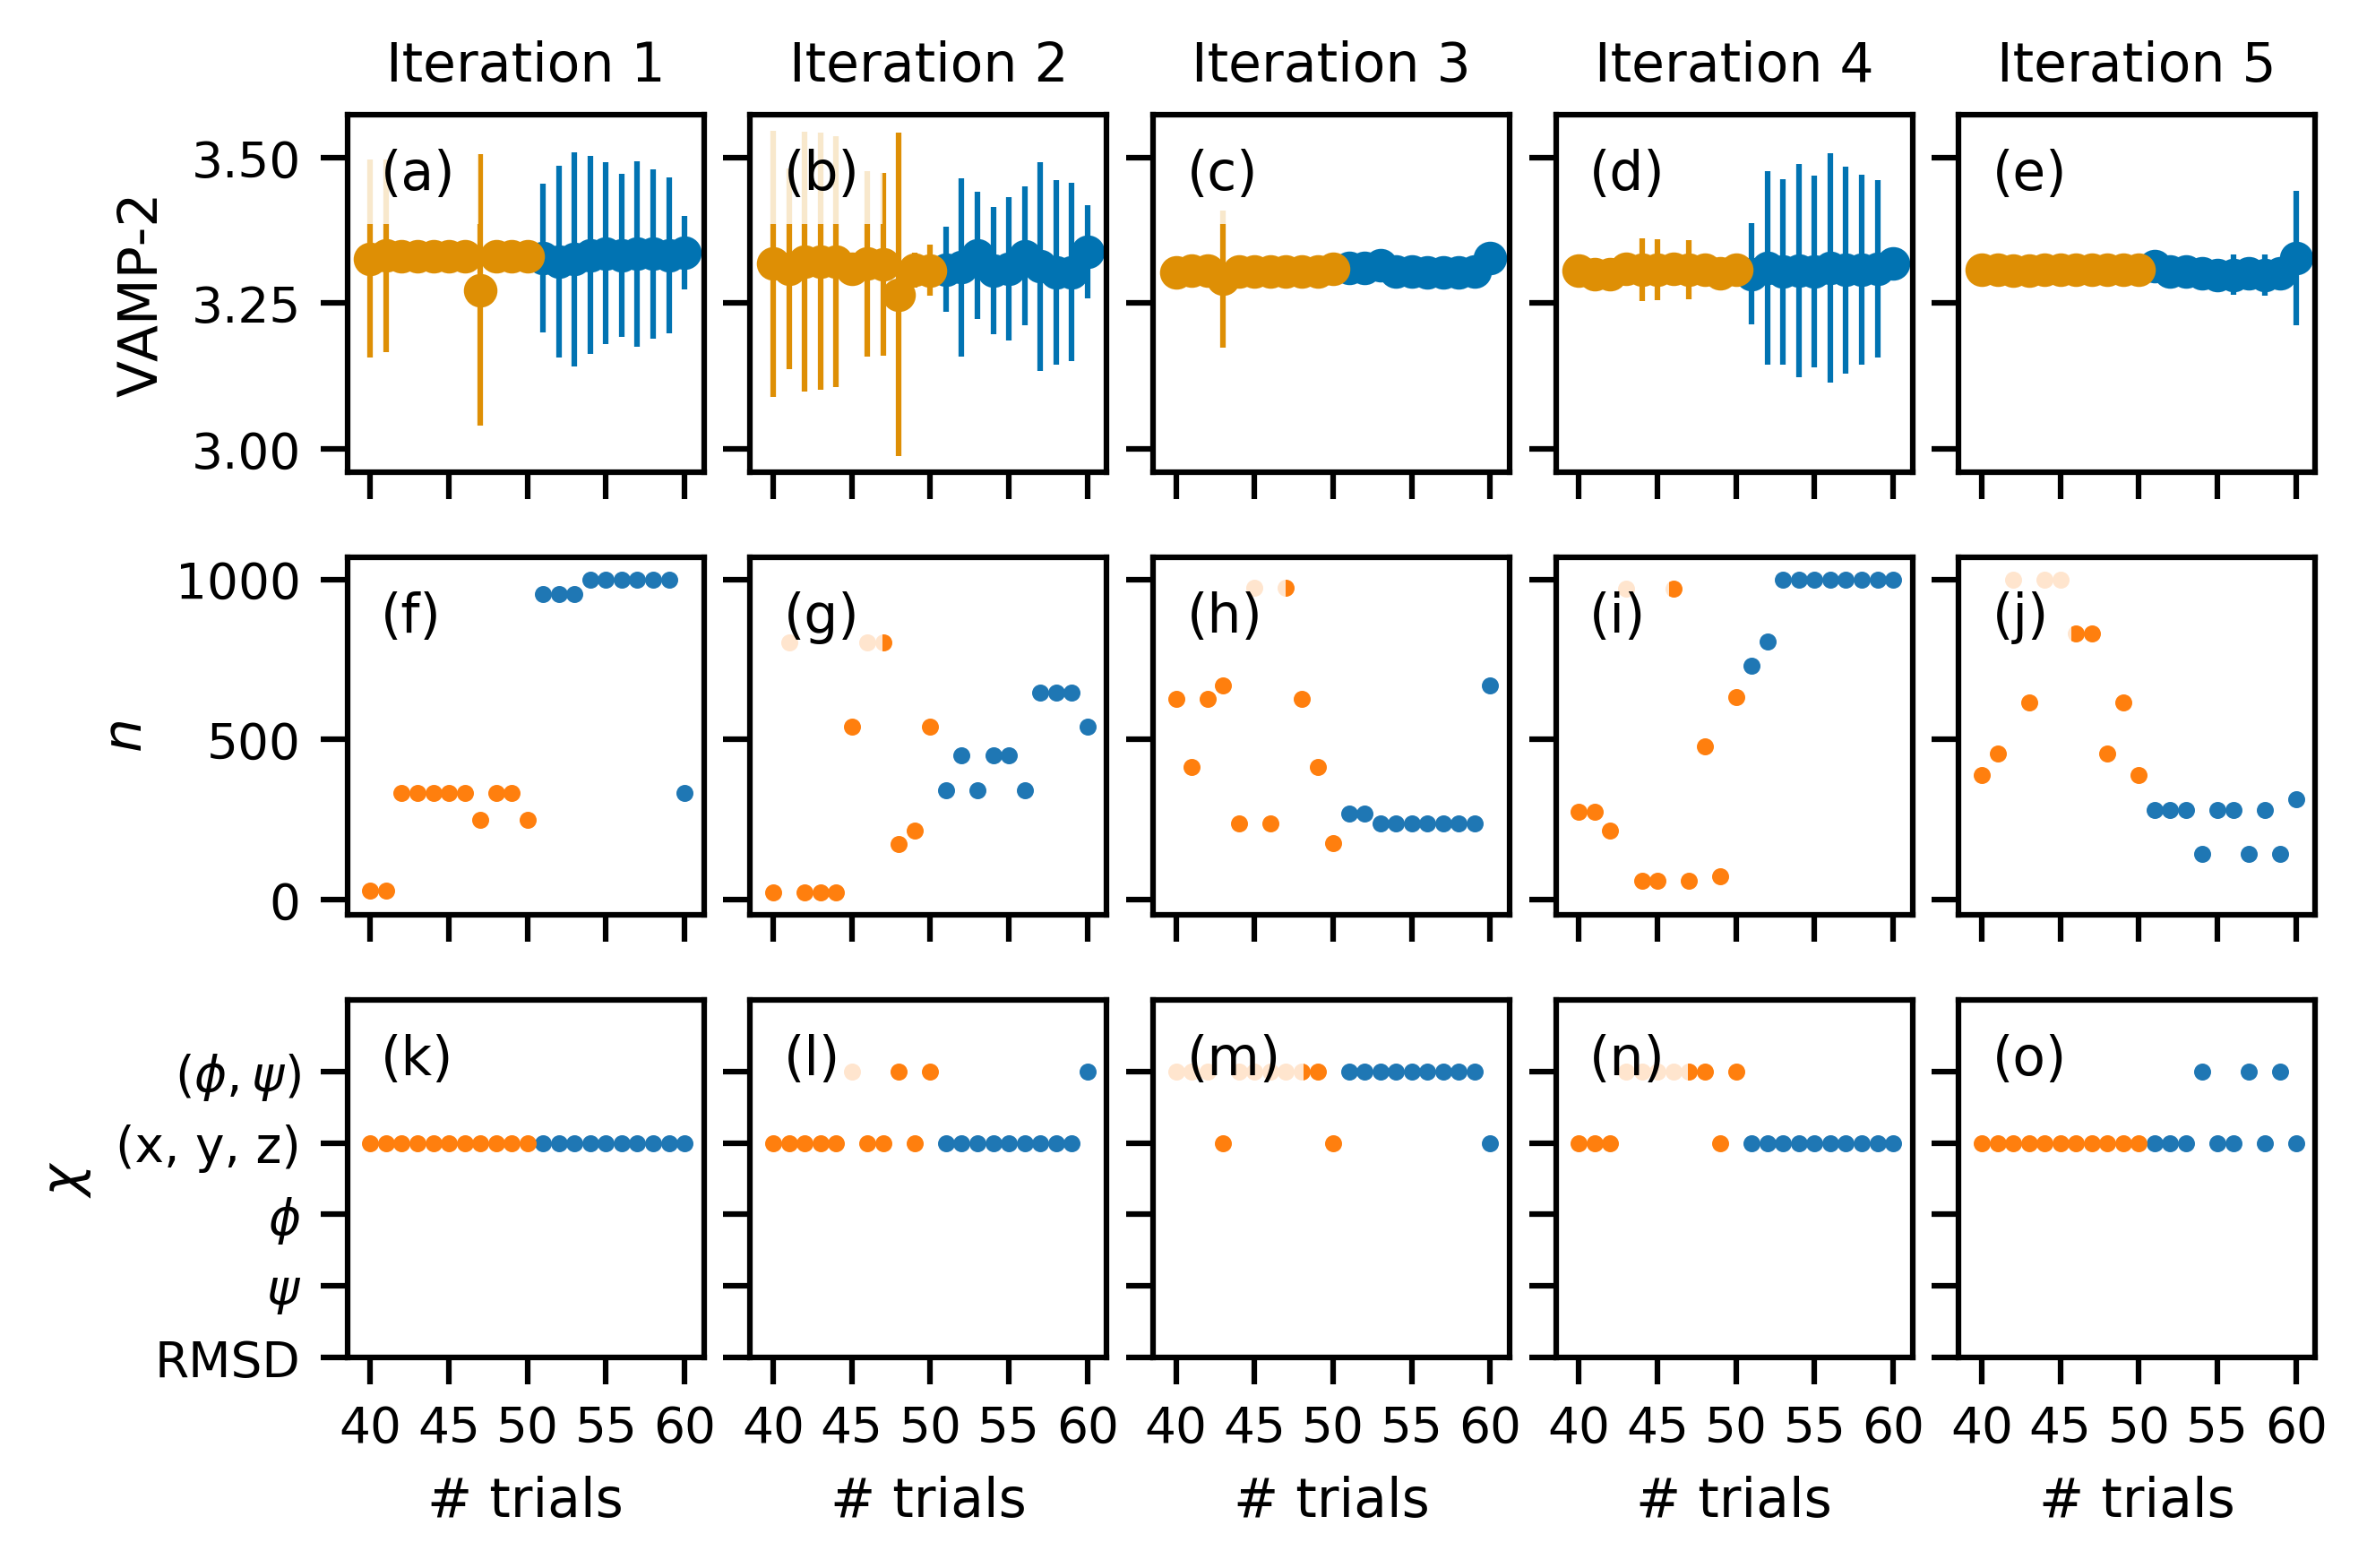
\includegraphics[width=\textwidth]{chapters/msm_optimization/figures/ala1_opt_traj_start_obs_50.png}
%         \caption{A tiger}
%         \label{fig:tiger}
%     \end{subfigure}
%     ~ %add desired spacing between images, e. g. ~, \quad, \qquad, \hfill etc. 
%     %(or a blank line to force the subfigure onto a new line)
% \end{figure}



\begin{figure}
    \centering
    \caption{Caption}
    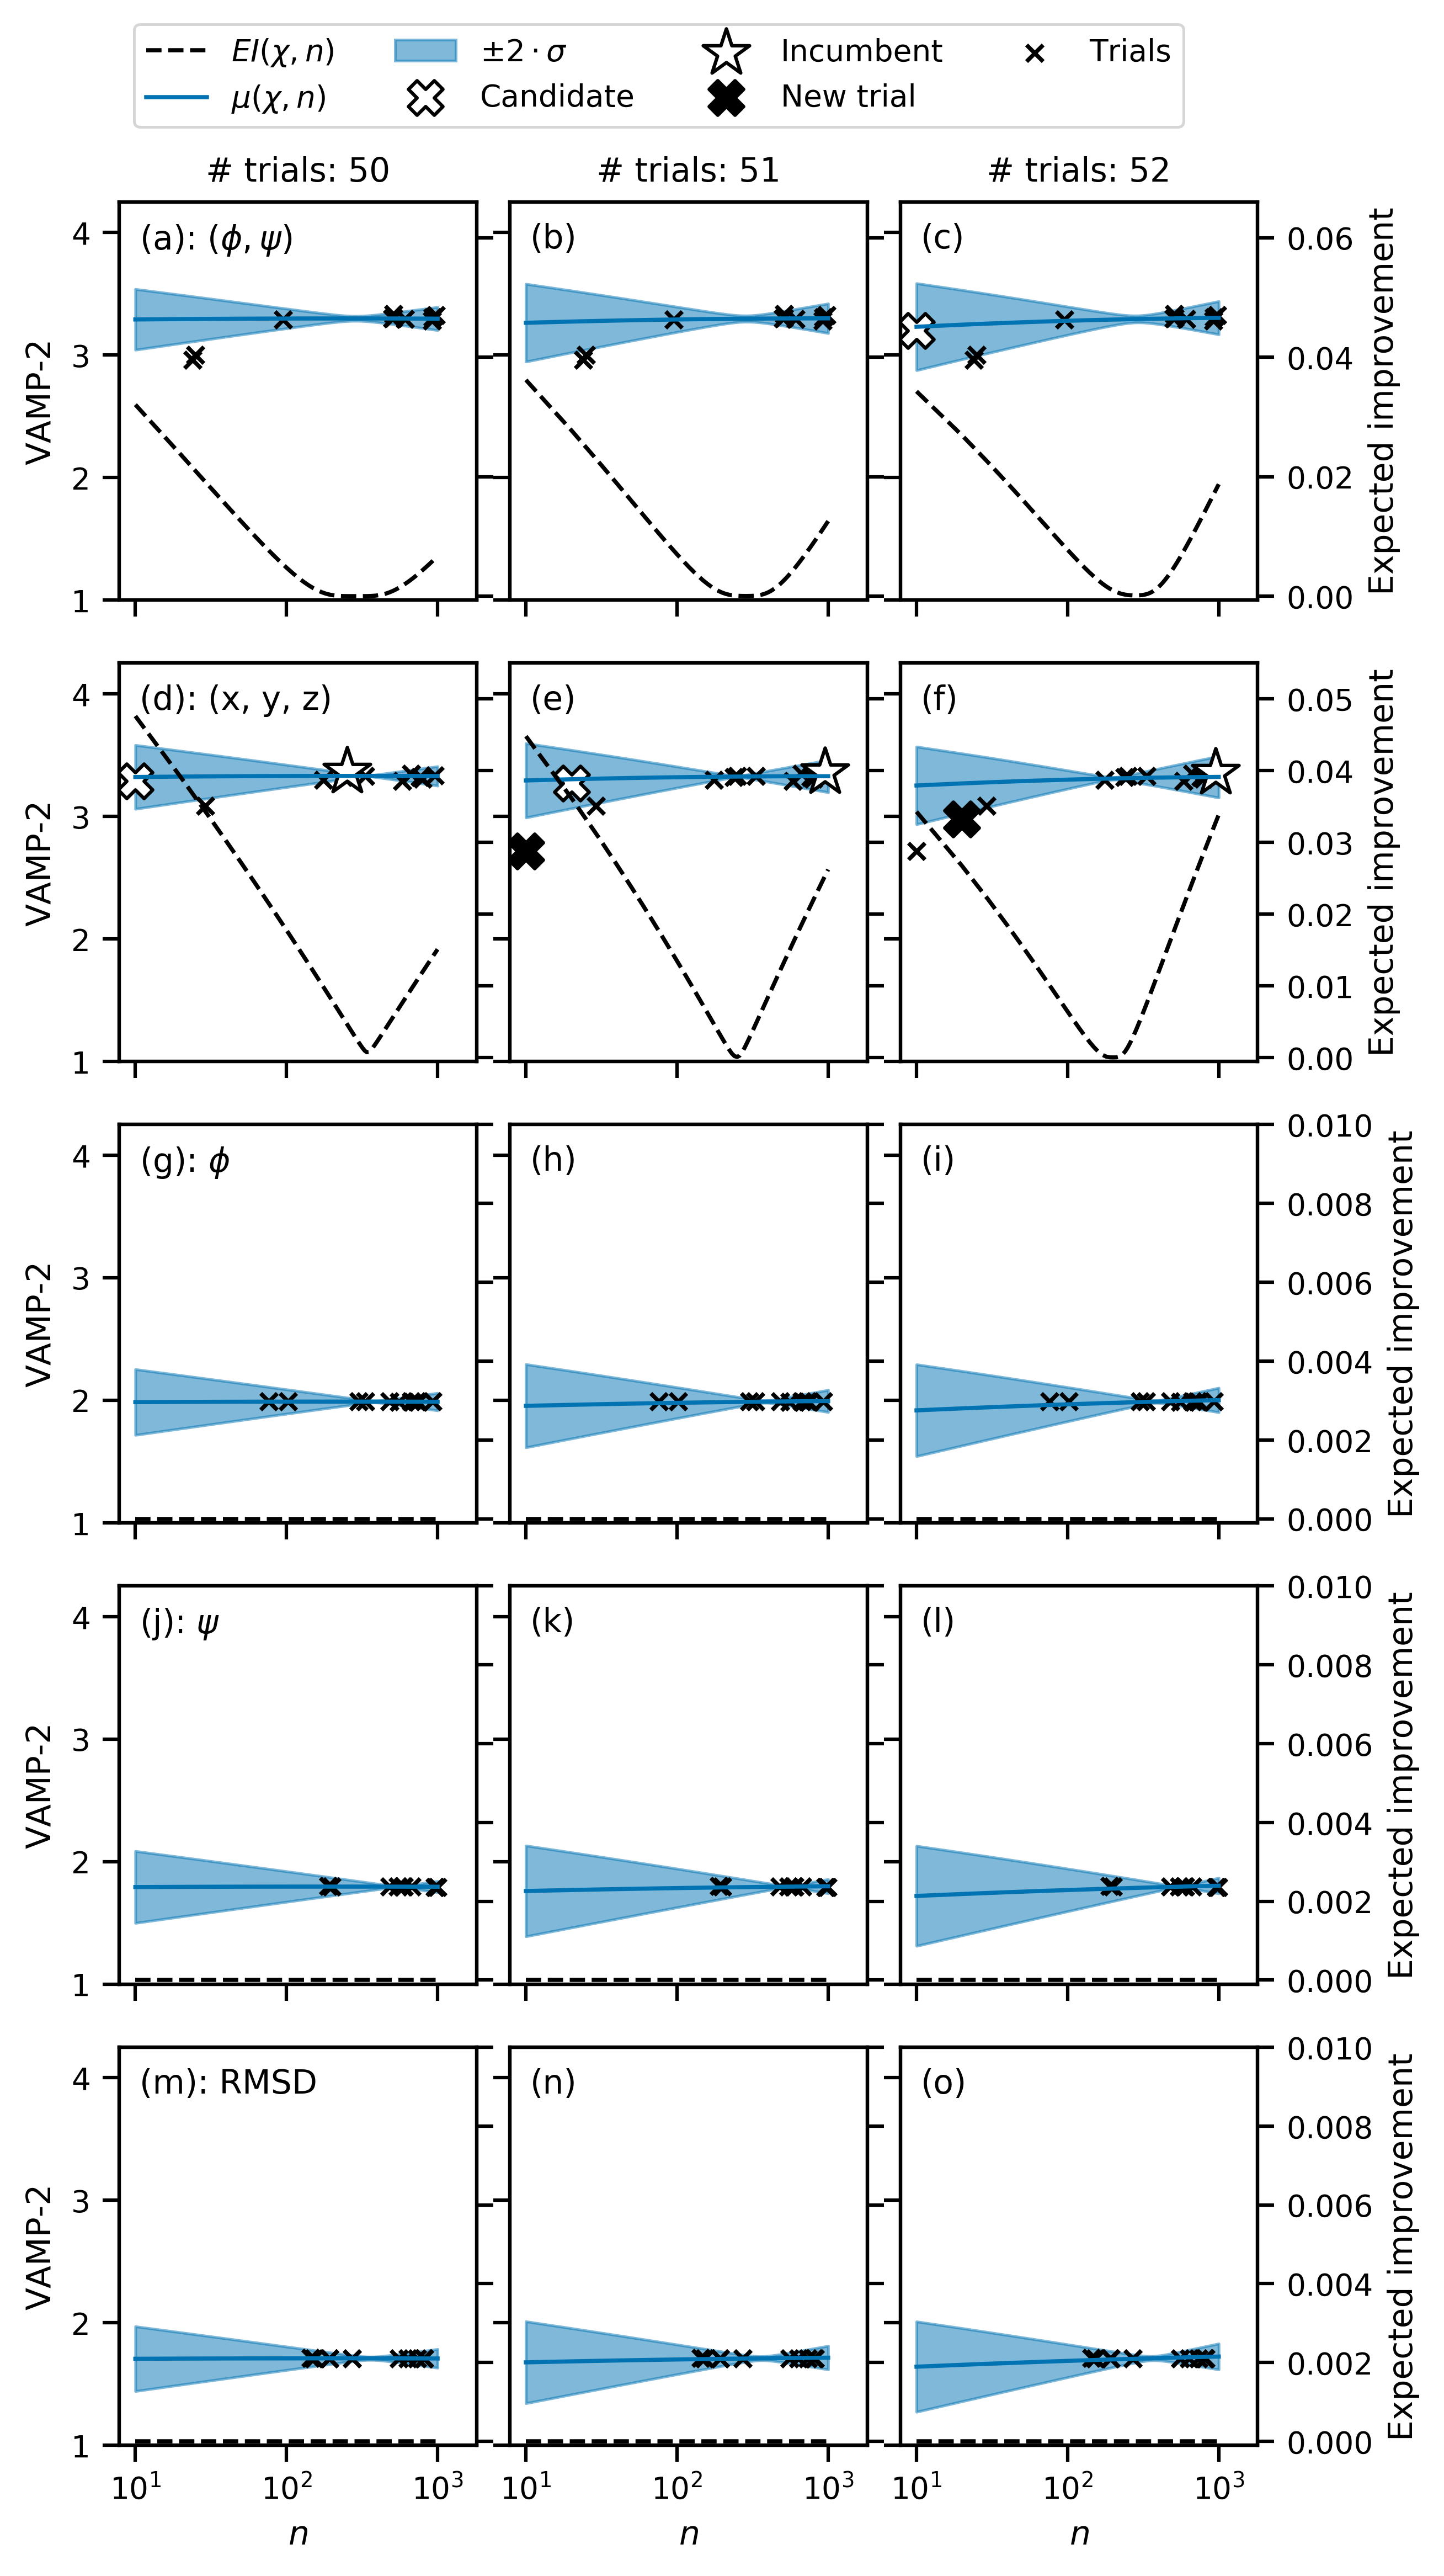
\includegraphics[height=0.8\textheight]{chapters/msm_optimization/figures/ala1_opt_explainer.png}
    \label{fig:ala1_opt_expl}
\end{figure}




\subsection{Aromatic Amine Dehydrogenase}

\subsubsection{Response surface}

The search space for AADH is shown in table \ref{tab:aadh_searchspace}. 

\begin{table}
    \caption{The hyperparameter search space for AADH. TICA was applied to every feature except RMSD. Torsional angles were given $\sin$, $\cos$ representations}
    \centering
    \begin{tabularx}{0.9\textwidth}{ |>{\raggedright\arraybackslash}l|l|>{\raggedright\arraybackslash}X| >{\raggedright\arraybackslash}X | } 
    \hline
    \textbf{Hyperparameter} & \textbf{Type} & \textbf{Search space} & \textbf{Details} \\
     \hline\hline
    Feature $\chi$ & Categorical & $(\phi, \psi, \chi)$ torsions &  \\
    & & RMSD &  Heavy atoms only\\ 
    & & Interatomic distances & Heavy atoms only, with variance threshold of $\ge\SI{1.5}{\angstrom}$ \\
    & & alpha-Carbon contacts & \\ 
    & & Heavy atom contacts & \\ 

    \hline
    TICA lag time, $\tau$ & Integer &\SIlist[list-final-separator = { ... }]{50;100;2000}{ps} & \\
    \hline
    TICA components, $m$& Integer &\numlist[list-final-separator = { ... }]{1;2;10} & \\
    \hline
    Cluster centres, $n$ & Integer & \numlist[list-final-separator = { ... }]{10;20;1000} &  KMeans \\
    
     \hline
    \end{tabularx}
    \label{tab:aadh_searchspace}
\end{table}



\begin{figure}
    \centering
    \caption{The $\operatorname{VAMP-2}$ scores of the hyperparameter trials for MSMs of AADH with featurized with (a) the $\phi, \psi, \chi$ torsions, (b) all distances between heavy atoms, (c) alpha-Carbon contact distances, (d) heavy atom contact distances, (e) root mean square deviation of heavy atoms. The trials are scored on the test set (blue) and on the training set (orange) for the H active site. The horizontal axis is the rank of the trial according to the test score. Each trial was scored with 20 iterations of 50:50 shuffle split cross validation. The error bars represent the 25th and 75th quantiles of the cross-validation folds. The features are ordered according to the mean of the their test scores.}
    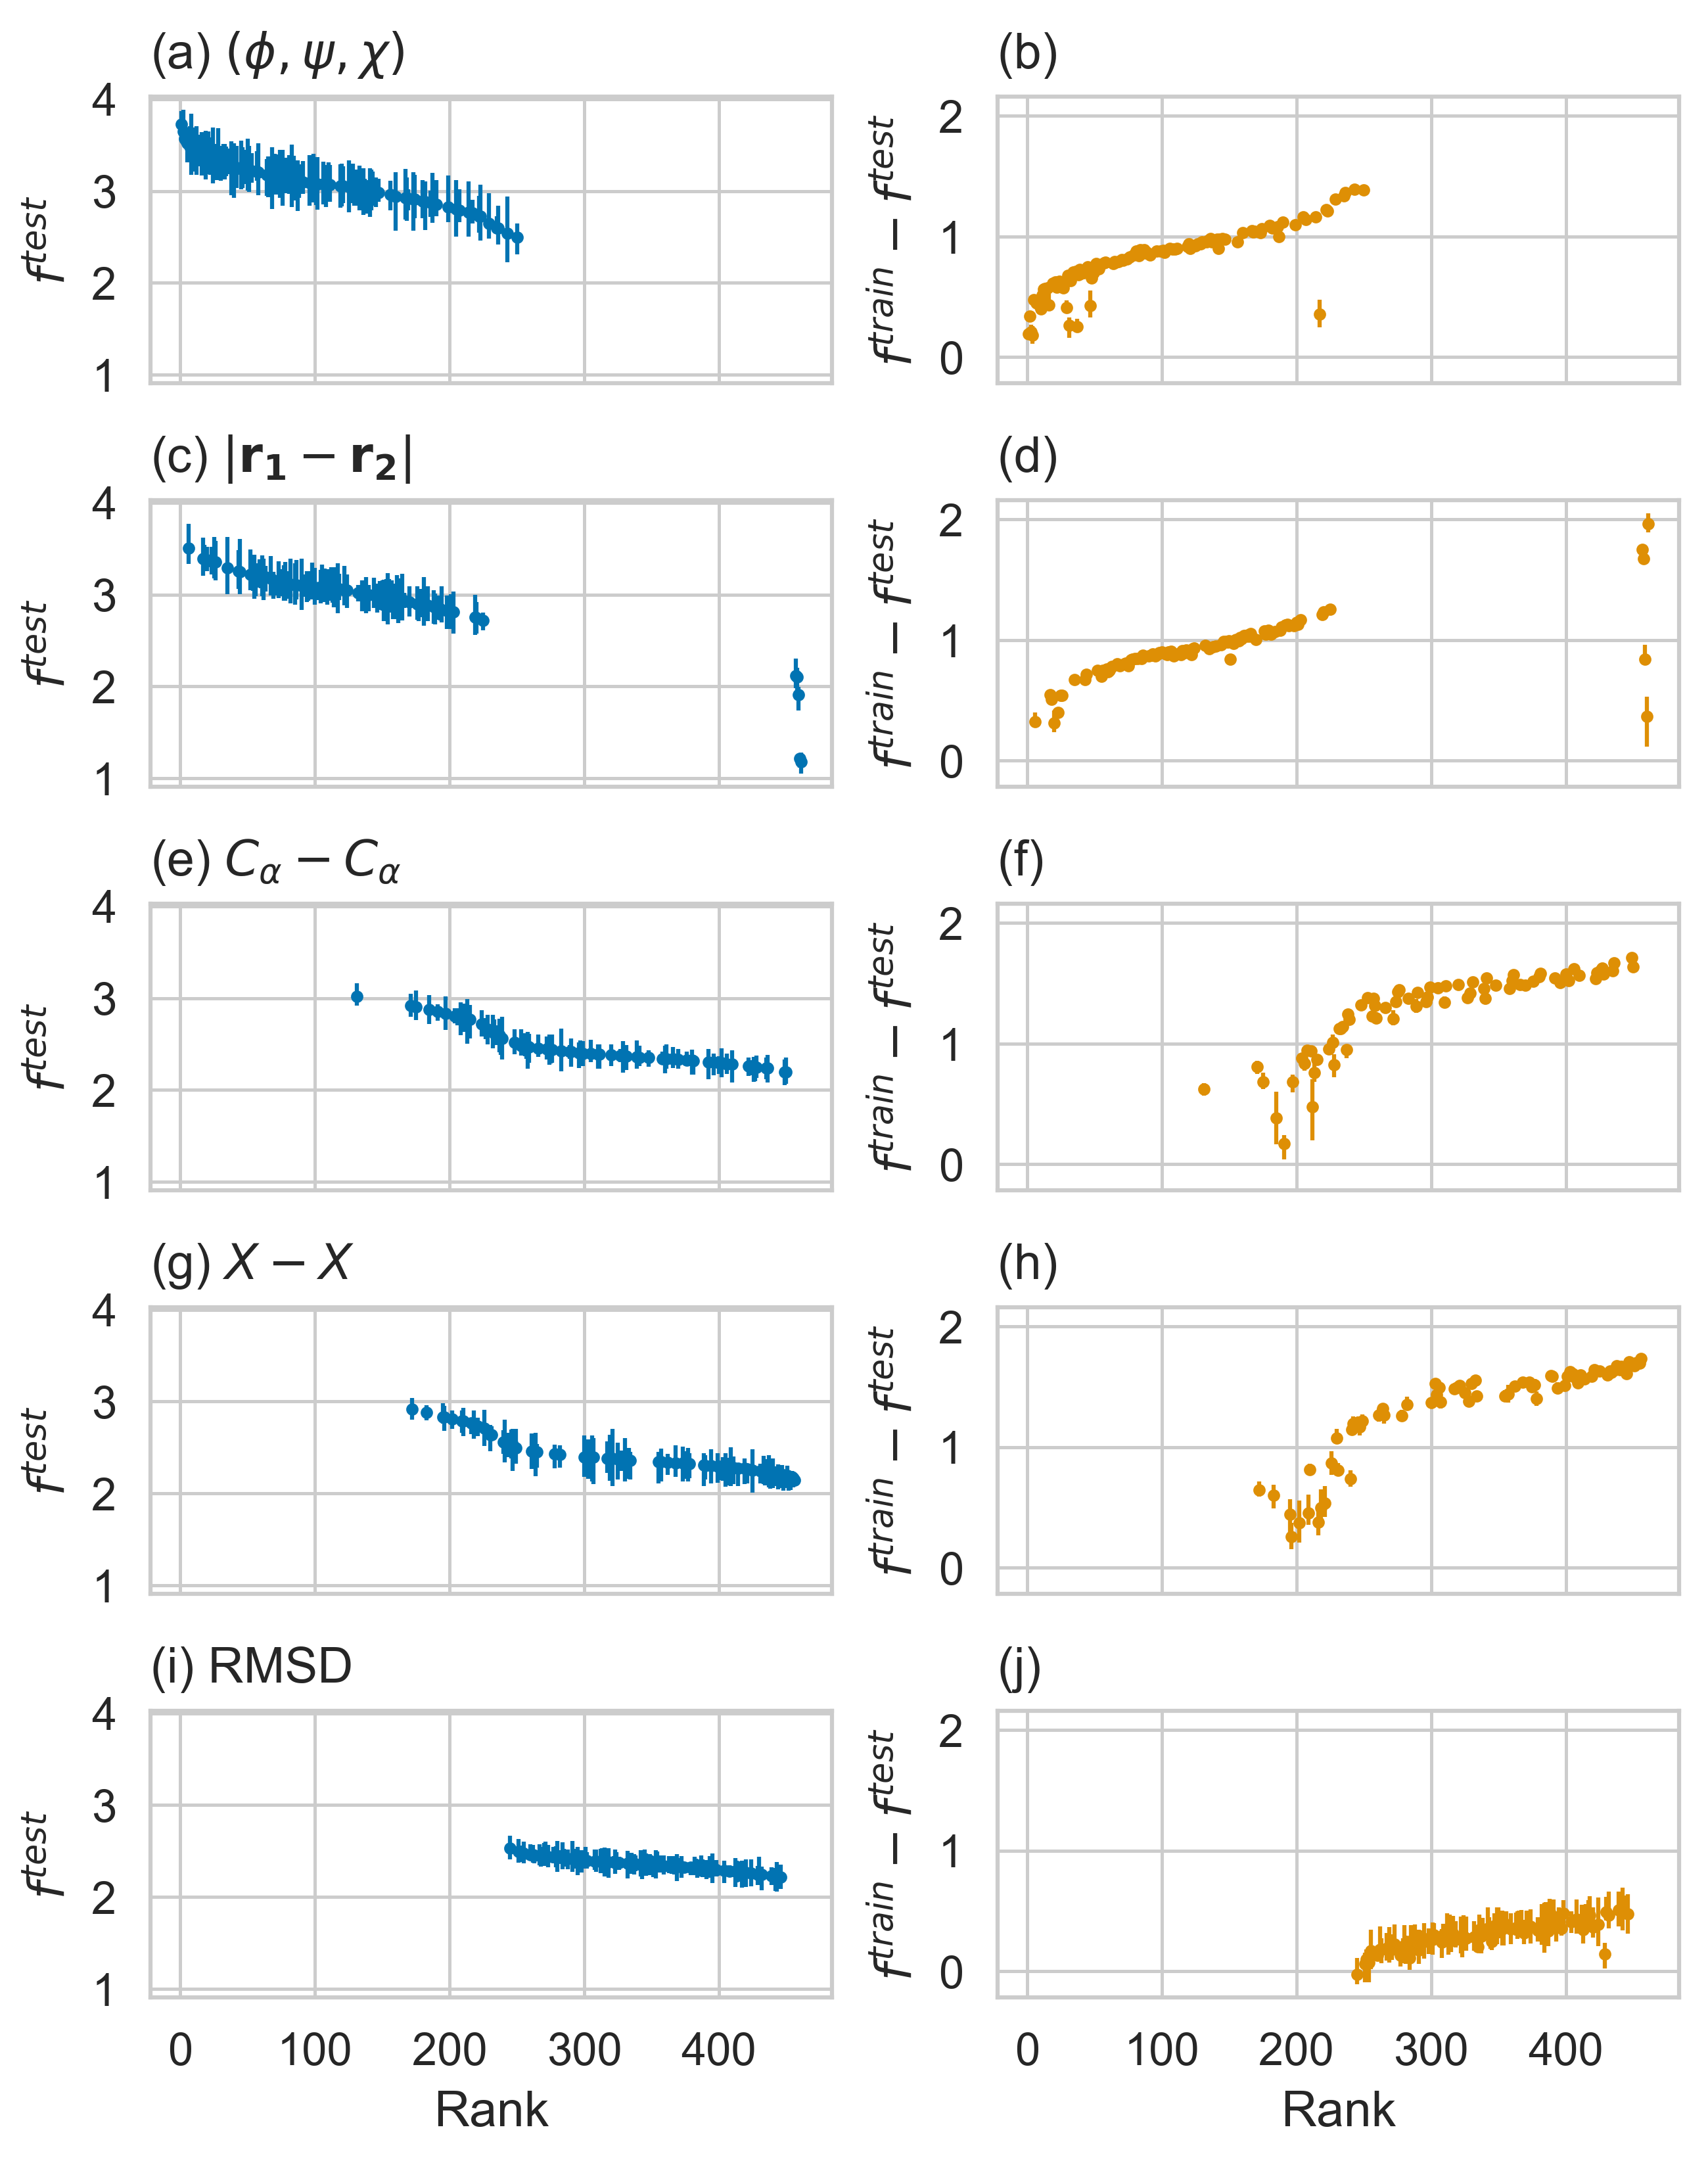
\includegraphics[width=0.8\textwidth]{chapters/msm_optimization/figures/aadh_train_test_results.png}
    \label{fig:aad_train_test}
\end{figure}


\begin{figure}
    \centering
    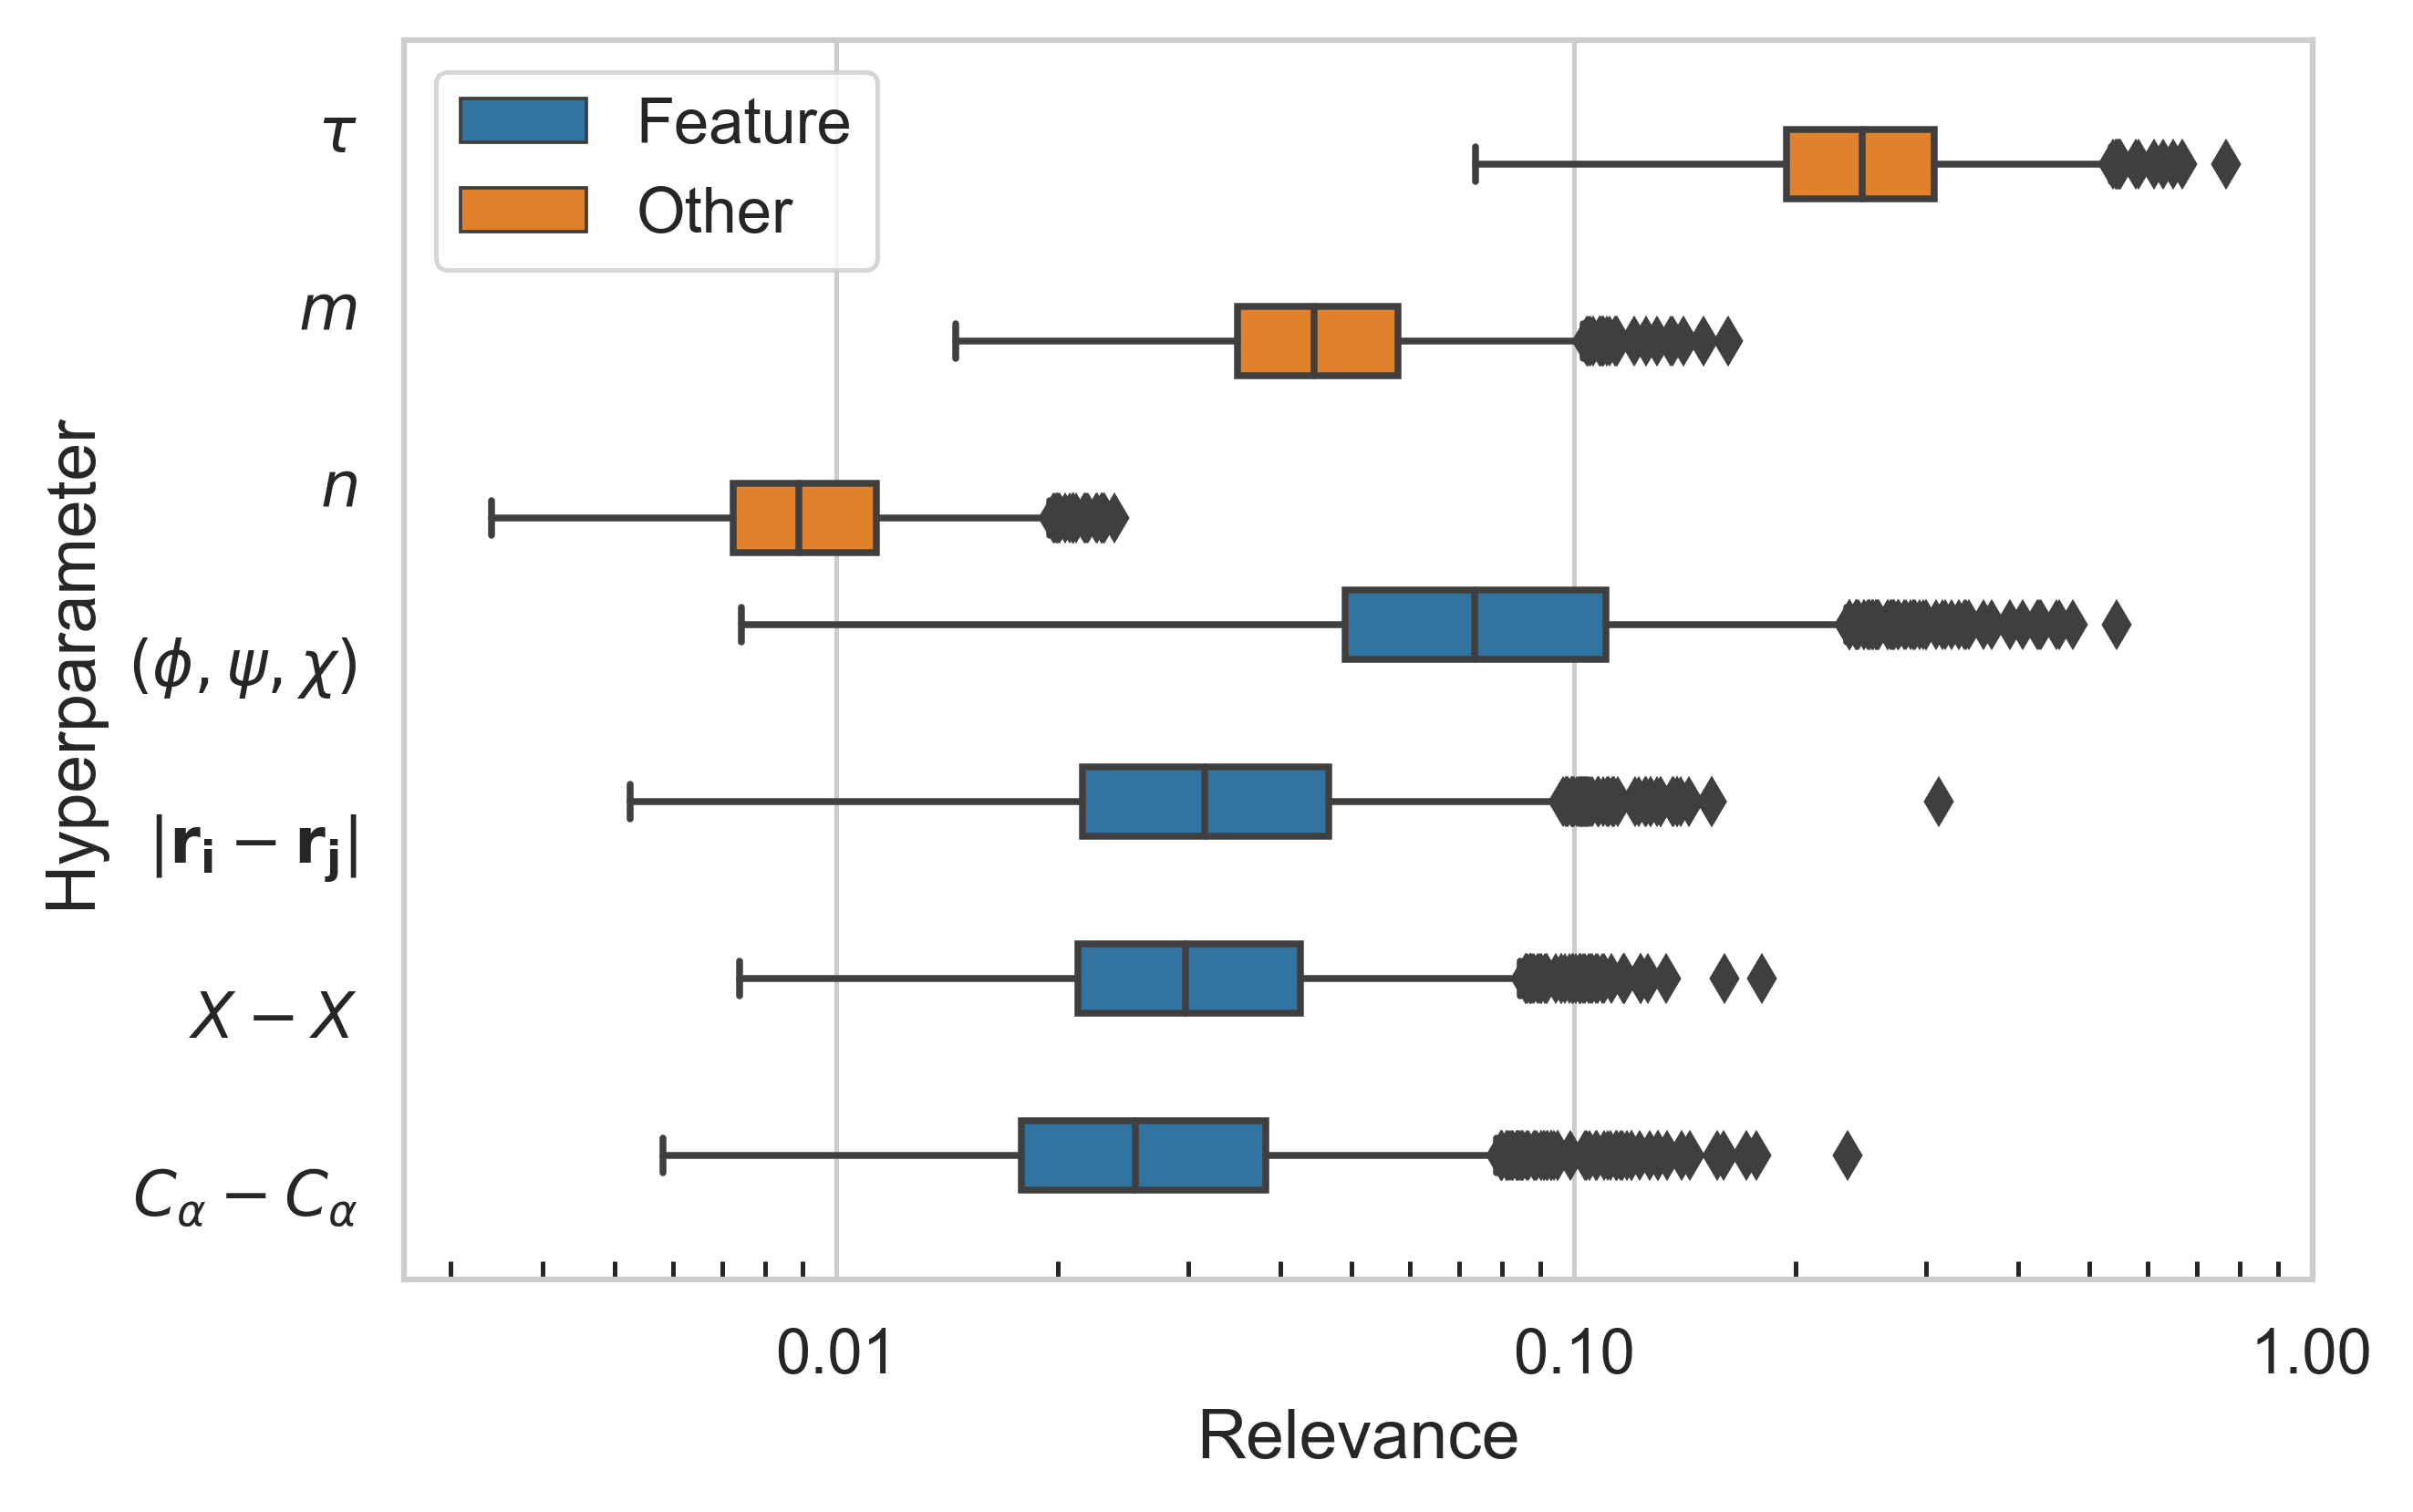
\includegraphics[width=0.8\textwidth]{chapters/msm_optimization/figures/AADH_relevance_d.png}
    \caption{Relevance of MSM for active site D}
    \label{fig:aadh_d_relevance}
\end{figure}

\subsubsection{Optimization}


\begin{figure}
    \centering
    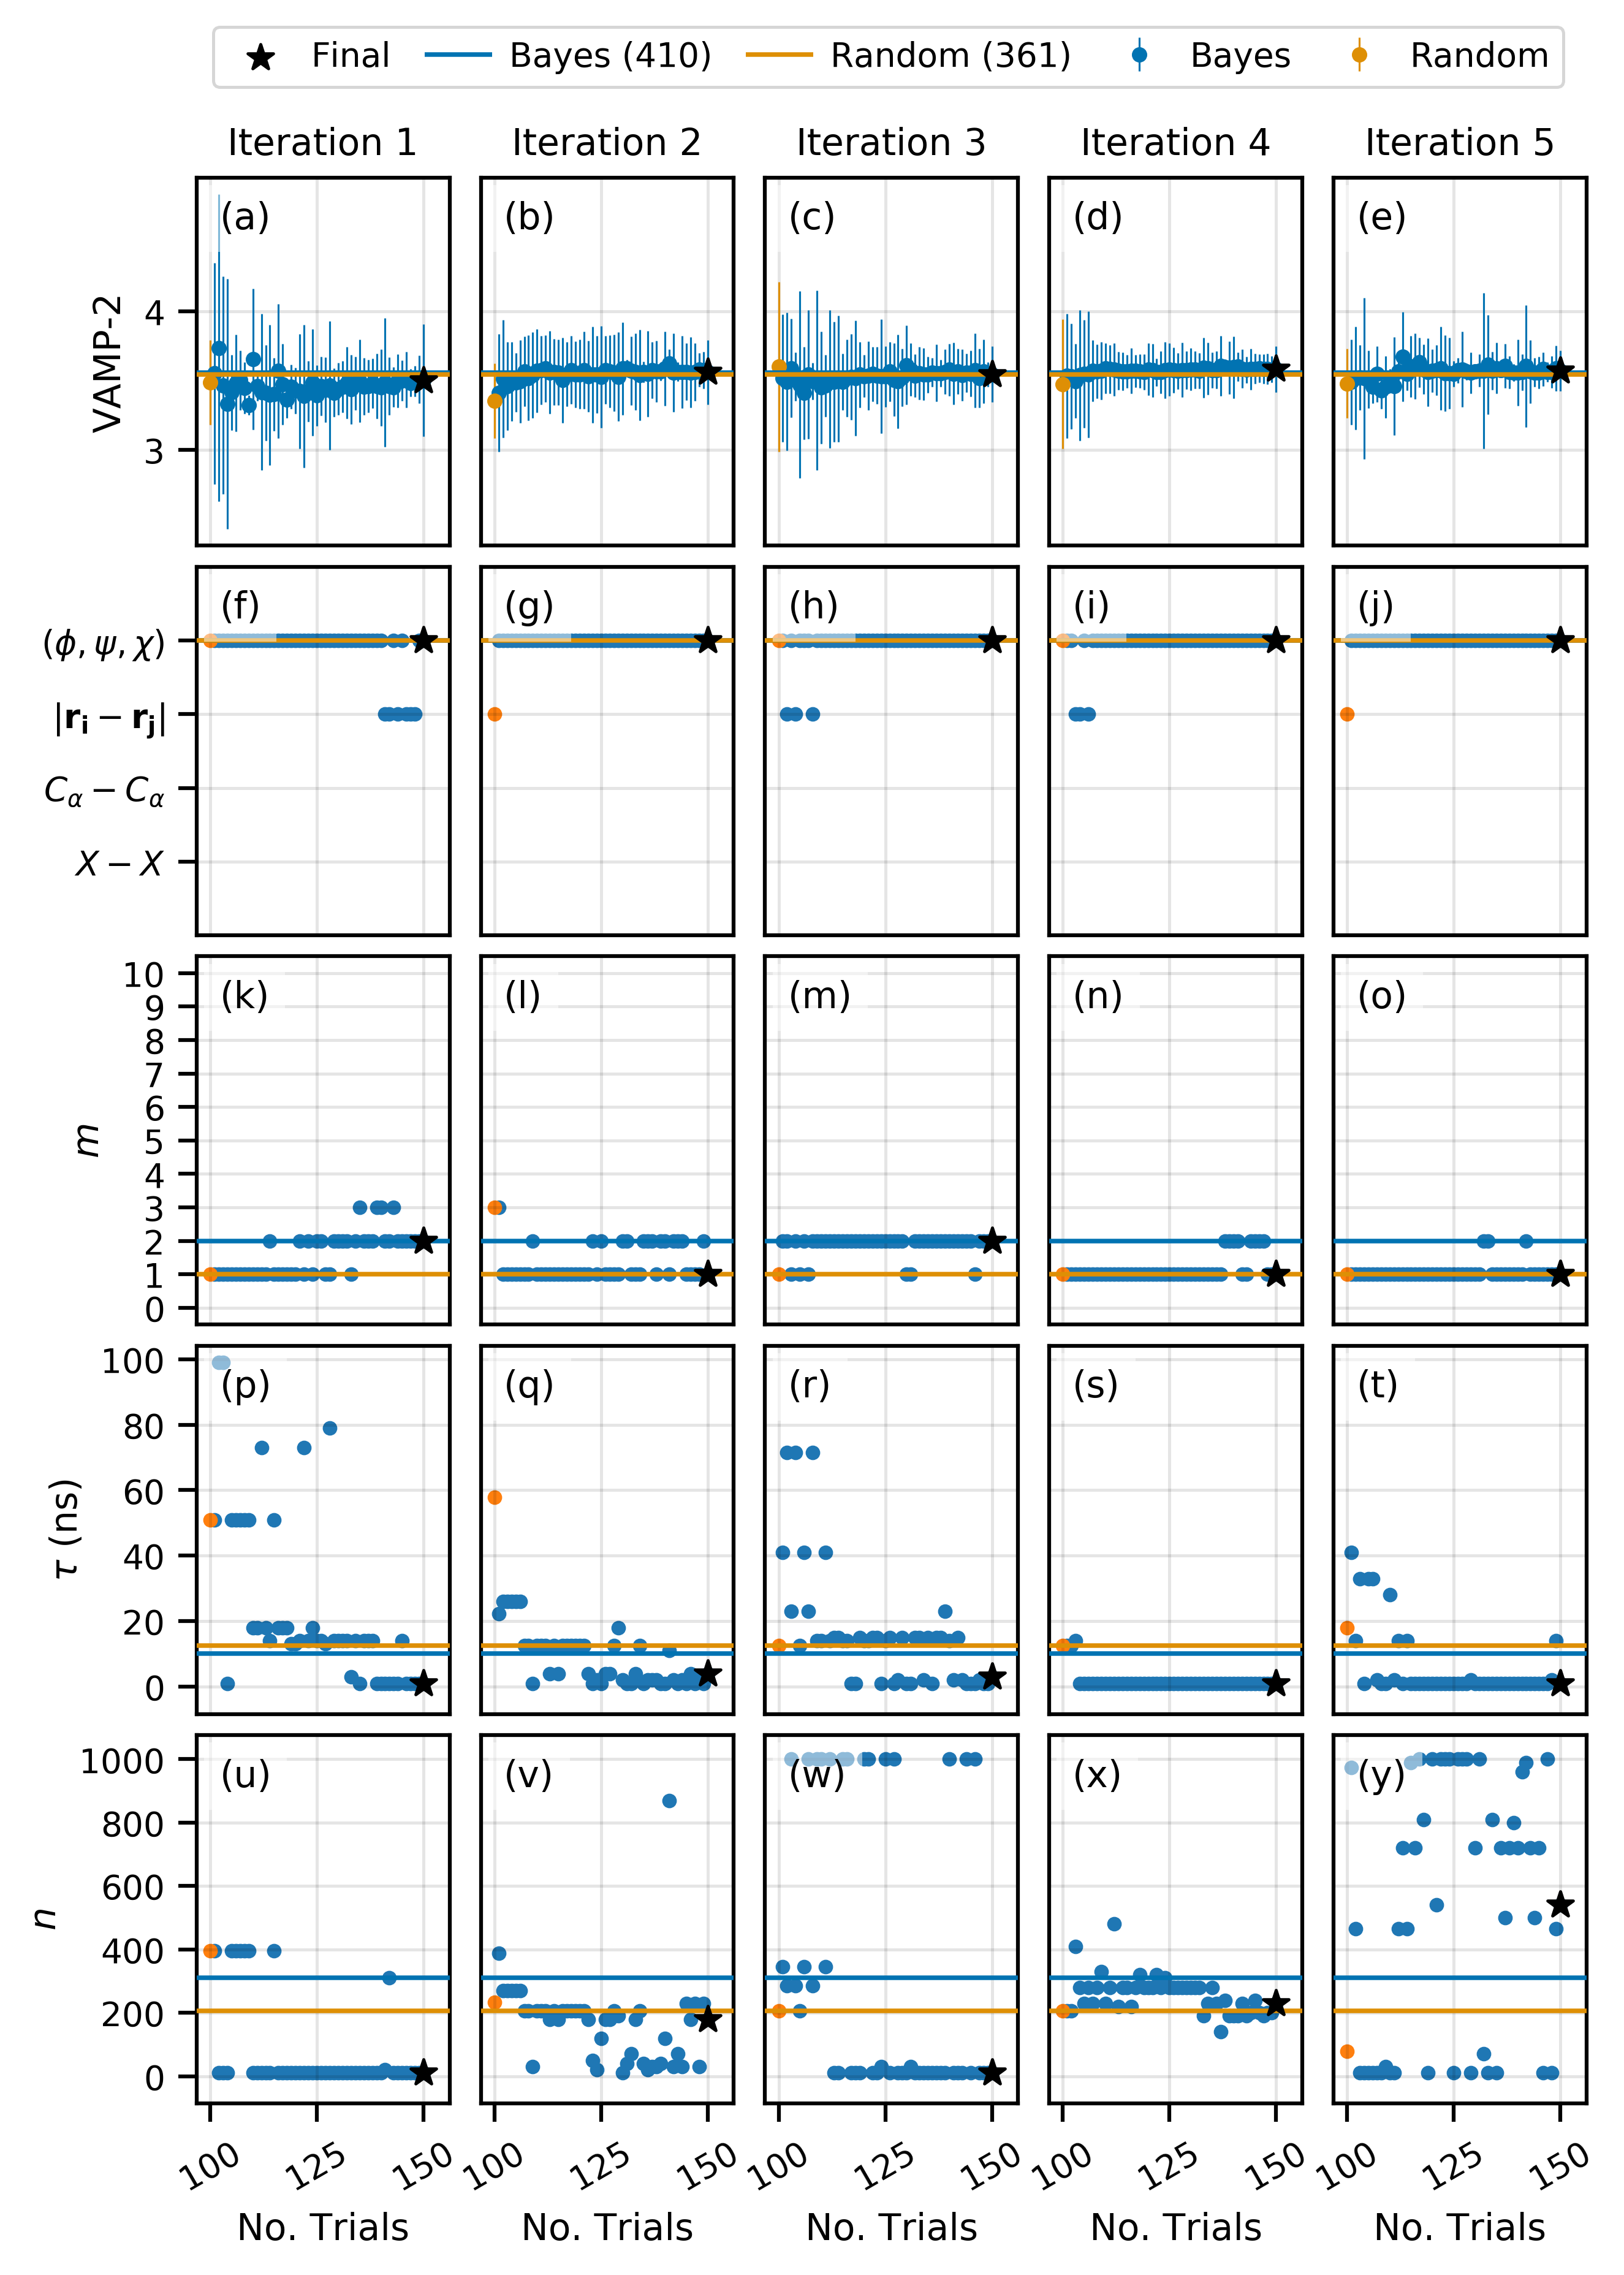
\includegraphics[width=0.8\textwidth]{chapters/msm_optimization/figures/aadh_opt_traj_act_s_d.png}
    \caption{Caption}
    \label{fig:aadh_opt_traj_d}
\end{figure}





\section{Conclusions}


\section{Appendix}\label{sec:msm_opt_app}

\subsection{Alanine Dipeptide}

\begin{figure}
    \centering
    \caption{The $\operatorname{VAMP-2}$ scores of the hyperparameter trials for MSMs of alanine dipeptide. The test response, $f^{test} = f(\chi, n; x^{test})$ is shown in blue, panels: a, c, e, g, i,  while the degree of over-fitting, $f^{train} - f^{test}$, is shown in orange, panels: b, d, f, h, j. Each row represents a different value of the feature ($\chi$) and the horizontal axis represent the number of clusters, ($n$). Each trial was scored with $20$ iterations of 50:50 shuffle split cross validation. The error bars represent the $25$th and $75$th quantiles of the cross-validation folds. 
    The features are ordered according to the mean of the their test scores.}
    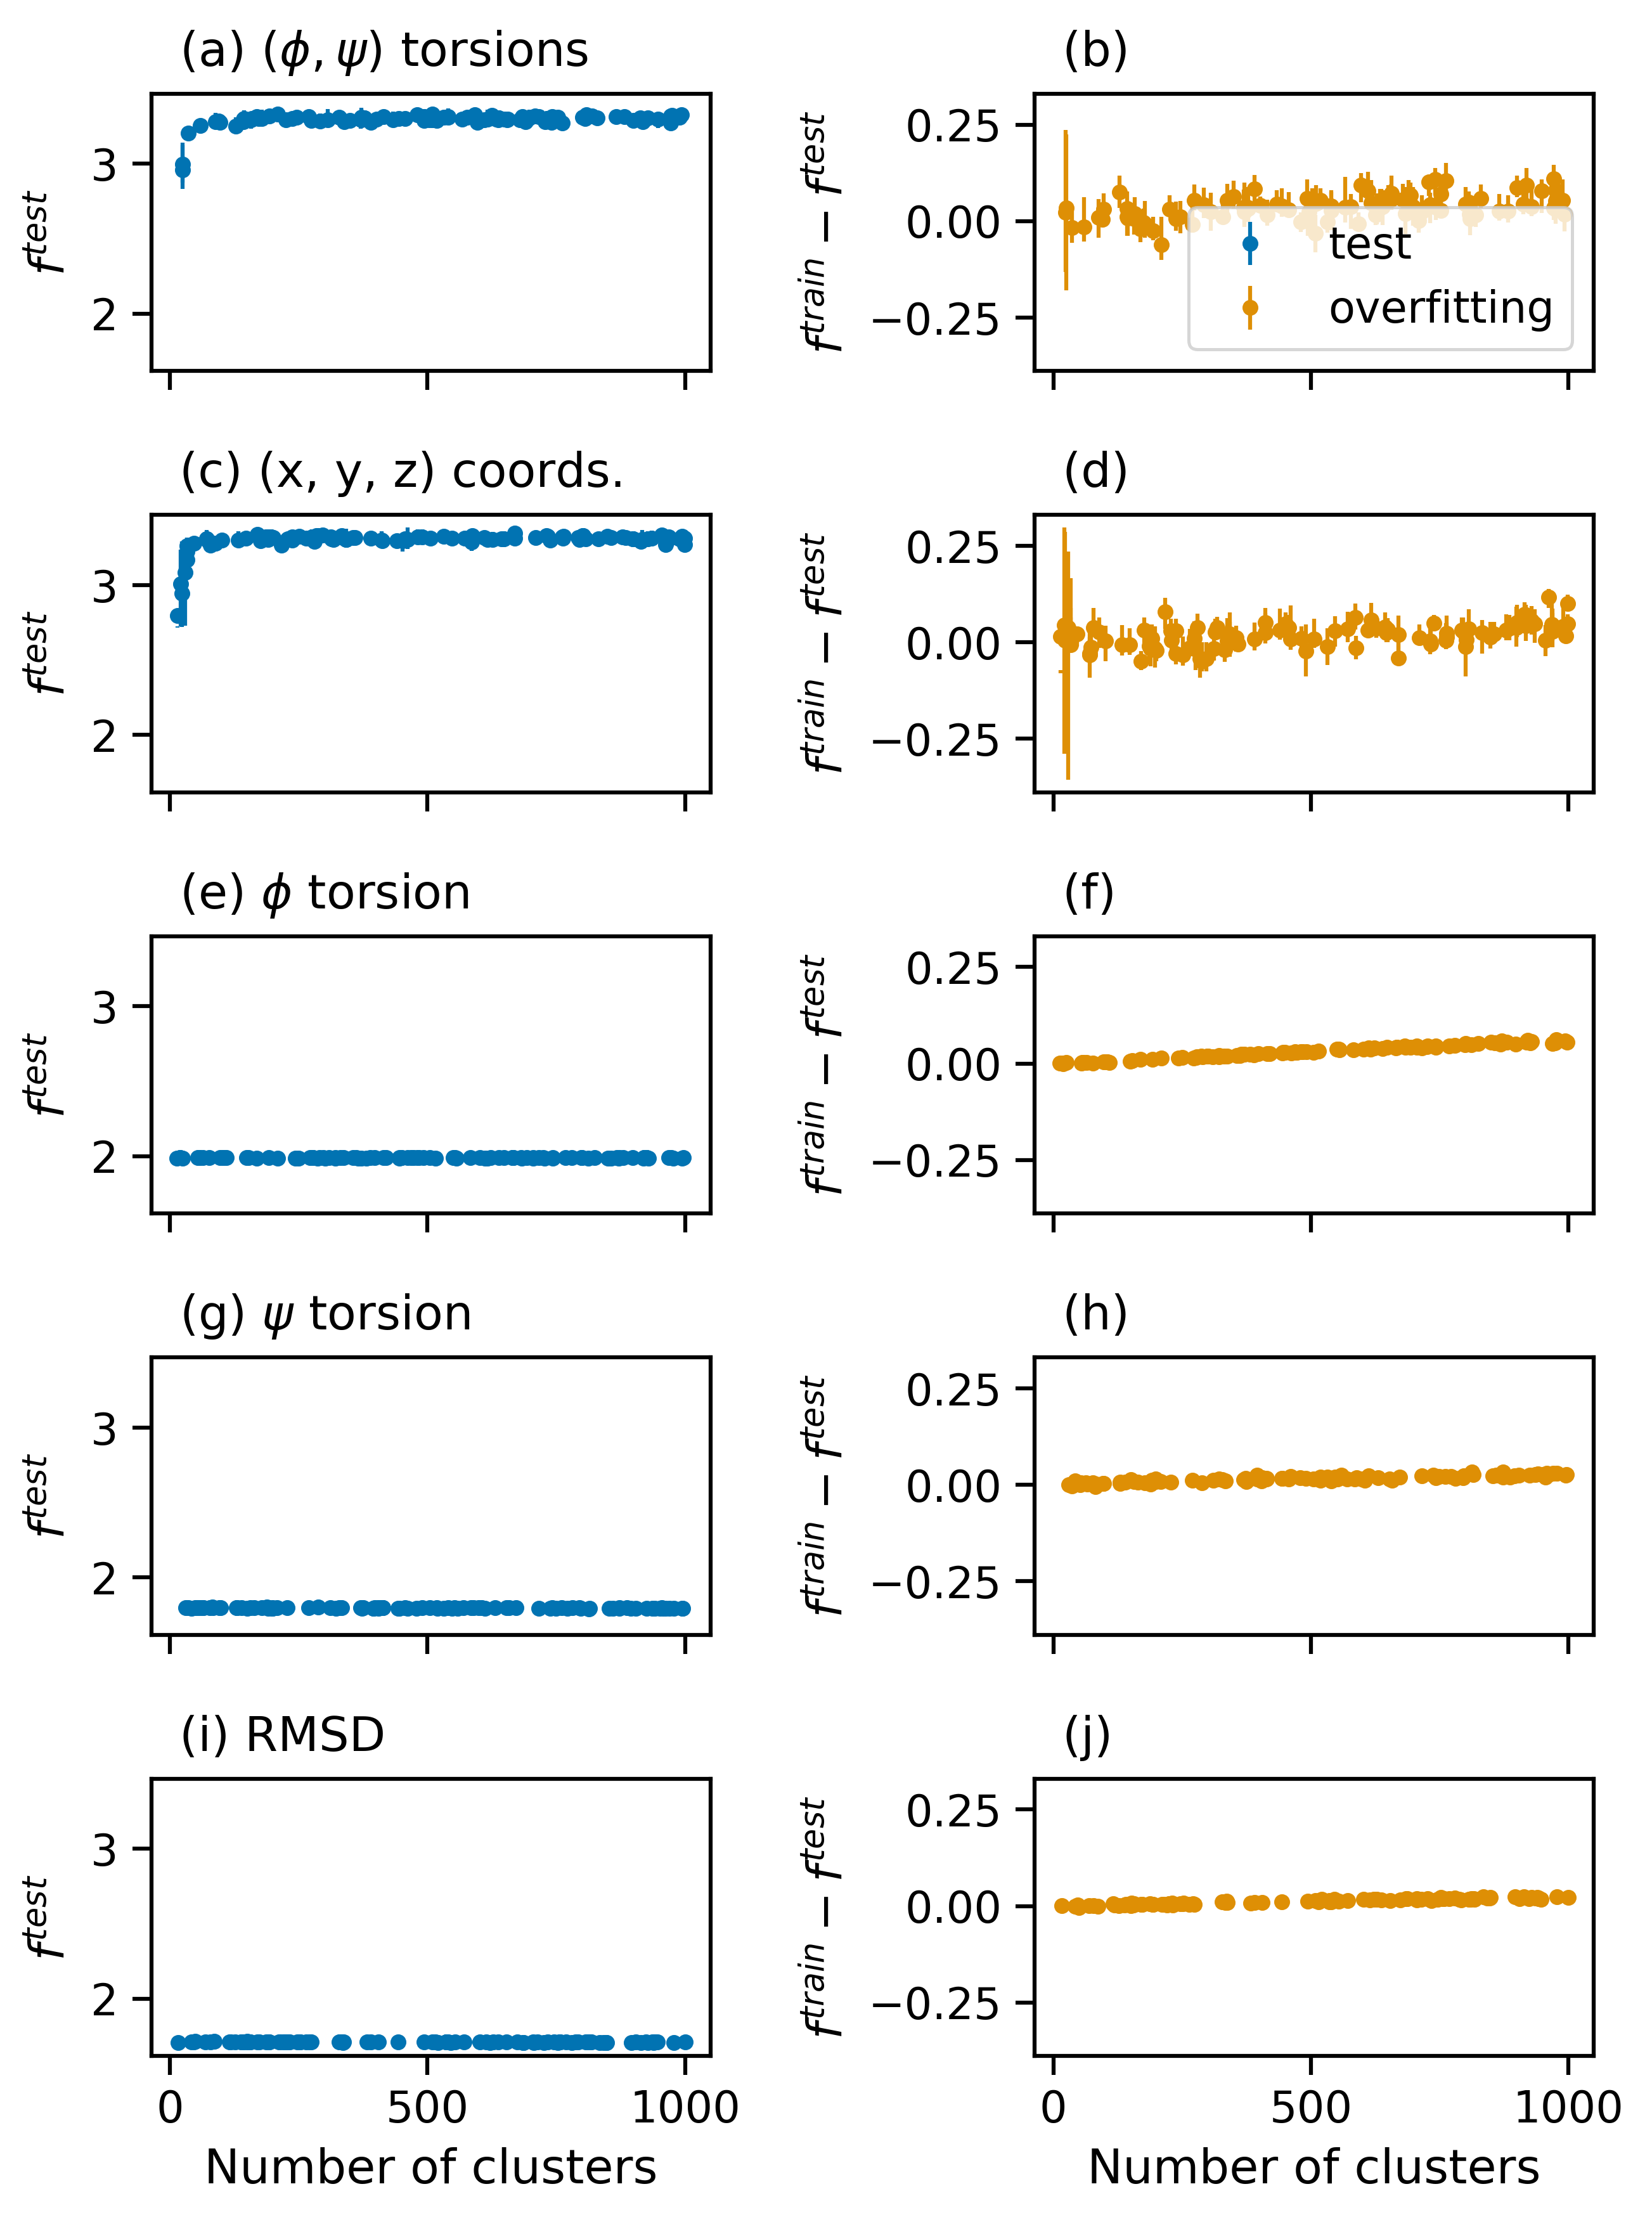
\includegraphics[height=0.8\textheight]{chapters/msm_optimization/figures/ala1_train_test_results.png}
    \label{fig:ala1_train_test}
\end{figure}

\begin{table}
    \centering
    \caption{ Moddel selection metrics othe response surface of Alanine Dipeptide. Standardized mean square error (SMSE) and mean standardized log loss (MSLL) for GP models of the response surface of MSMs for alanine dipeptide, using different transformations of $n$ ($T(n)$) and different kernels. Each GP model used a mean prior of zero, and all other parameters were estimated by maximizing the marginal likelihood. All values were calculated using 10-fold cross-validation.}
    \begin{tabular}{|l|l|c|c|c|}
    \hline
    T(n) &       Name &  SMSE &    MSLL \\
    \hline\hline
     $\log{(n)}$ &  Exponential & 0.0012 & -3.9963 \\
      &  Mat{\'e}rn 3-2  & 0.0010 & -4.1712 \\
      &  Mat{\'e}rn 5-2  & 0.0007 & -4.2369 \\
      &  Gaussian & 0.0011 & -4.0892 \\
     $I(n)$ &  Exponential  & 0.0027 & -2.9733 \\
      &  Mat{\'e}rn 3-2  & 0.0025 & -3.4218 \\
      &  Mat{\'e}rn 5-2  & 0.0023 & -3.8172 \\
      &  Gaussian & 0.0032 & -4.1239 \\
    \hline
    \end{tabular}
    \label{tab:ala2_fit_results}
\end{table}

\begin{table}
    \centering
    \caption{Model selection metrics for the response surface of AADH using all hyperparameter trials ($N=361$, except those for $\chi=$RMSD). The Mean Standardized Log Loss (MSLL) and Standardized Mean Square Error (SMSE) where calculated using 10 fold cross validation. Only those models which had both $\mathrm{MSLL}<0$ and $\mathrm{SMSE}<1$ were ranked. The total rank is calculated as rank of $\sqrt{R_{MSLL}^{2}+R_{SMSE}^2}$. Where the overall rank was tied, the first model appearing in the table was ranked higher. }
    \label{tab:aadh_rsm_metrics_all_data}
    \begin{tabularx}{1\textwidth}{|llllrr >{\raggedright\arraybackslash}X>{\raggedright\arraybackslash}X>{\raggedright\arraybackslash}X|}
    \hline
    $T(\tau)$ & $T(m)$ & $T(n)$ & Kernel & MSLL &   SMSE & Rank (MSLL) & Rank (SMSE) & Rank (Total)\\
    \hline\hline
    $I({\tau})$ & $I({m})$ & $I({n})$ & Exponential & -0.1298 & 0.3087 &       1.0 &       1.0 &  1.0 \\
                   &             & $\log({n})$ & Exponential &  0.0050 & 0.2964 &         - &         - &    - \\
                   & $\log({m})$ & $I({n})$ & Exponential &  0.0521 & 0.3118 &         - &         - &    - \\
                   &             & $\log({n})$ & Exponential &  0.5633 & 0.3815 &         - &         - &    - \\
    $\log({\tau})$ & $I({m})$ & $I({n})$ & Exponential &  0.1967 & 0.3436 &         - &         - &    - \\
                   &             & $\log({n})$ & Exponential &  0.4959 & 0.3231 &         - &         - &    - \\
                   & $\log({m})$ & $I({n})$ & Exponential &  0.5128 & 0.4365 &         - &         - &    - \\
                   &             & $\log({n})$ & Exponential &  1.0267 & 0.4201 &         - &         - &    - \\
    $I({\tau})$ & $I({m})$ & $I({n})$ & M32 &  1.5680 & 0.2893 &         - &         - &    - \\
                   &             & $\log({n})$ & M32 &  1.9193 & 0.2960 &         - &         - &    - \\
                   & $\log({m})$ & $I({n})$ & M32 &  3.1385 & 0.2775 &         - &         - &    - \\
                   &             & $\log({n})$ & M32 &  2.0358 & 0.2818 &         - &         - &    - \\
    $\log({\tau})$ & $I({m})$ & $I({n})$ & M32 &  6.9015 & 0.3203 &         - &         - &    - \\
                   &             & $\log({n})$ & M32 &  7.7182 & 0.3406 &         - &         - &    - \\
                   & $\log({m})$ & $I({n})$ & M32 &  7.9209 & 0.3257 &         - &         - &    - \\
                   &             & $\log({n})$ & M32 &  3.0002 & 0.3472 &         - &         - &    - \\
    $I({\tau})$ & $I({m})$ & $I({n})$ & M52 &  3.6517 & 0.3029 &         - &         - &    - \\
                   &             & $\log({n})$ & M52 &  3.8316 & 0.3090 &         - &         - &    - \\
                   & $\log({m})$ & $I({n})$ & M52 &  8.6574 & 0.2991 &         - &         - &    - \\
                   &             & $\log({n})$ & M52 &  3.7354 & 0.3238 &         - &         - &    - \\
    $\log({\tau})$ & $I({m})$ & $I({n})$ & M52 &  8.9207 & 0.3679 &         - &         - &    - \\
                   &             & $\log({n})$ & M52 & 11.8753 & 0.4064 &         - &         - &    - \\
                   & $\log({m})$ & $I({n})$ & M52 & 12.7637 & 0.3722 &         - &         - &    - \\
                   &             & $\log({n})$ & M52 & 13.6735 & 0.3475 &         - &         - &    - \\
    $I({\tau})$ & $I({m})$ & $I({n})$ & RBF &     inf &    inf &         - &         - &    - \\
                   &             & $\log({n})$ & RBF &  9.3618 & 0.3256 &         - &         - &    - \\
                   & $\log({m})$ & $I({n})$ & RBF &  5.9123 & 0.3022 &         - &         - &    - \\
                   &             & $\log({n})$ & RBF &     inf &    inf &         - &         - &    - \\
    $\log({\tau})$ & $I({m})$ & $I({n})$ & RBF & 17.4786 & 0.4551 &         - &         - &    - \\
                   &             & $\log({n})$ & RBF & 16.7568 & 0.3556 &         - &         - &    - \\
                   & $\log({m})$ & $I({n})$ & RBF & 16.7412 & 0.5026 &         - &         - &    - \\
                   &             & $\log({n})$ & RBF & 24.3199 & 0.4986 &         - &         - &    - \\
    \hline
    \end{tabularx}
\end{table}



\begin{table}
    \centering
    \caption{Model selection metrics for the response surface of an MSM of AADH, data subset 1, $N=100$, except those for $\chi=$RMSD). The Mean Standardized Log Loss (MSLL) and Standardized Mean Square Error (SMSE) where calculated using 10 fold cross validation. Only those models which had both $\mathrm{MSLL}<0$ and $\mathrm{SMSE}<1$ were ranked. The total rank is calculated as rank of $\sqrt{R_{MSLL}^{2}+R_{SMSE}^2}$. Where the overall rank was tied, the first model appearing in the table was ranked higher. }
    \label{tab:aadh_rsm_metrics_iter_1}
    \begin{tabularx}{1\textwidth}{|llllrr >{\raggedright\arraybackslash}X>{\raggedright\arraybackslash}X>{\raggedright\arraybackslash}X|}
    \hline
    $T(\tau)$ & $T(m)$ & $T(n)$ & Kernel & MSLL &   SMSE & Rank (MSLL) & Rank (SMSE) & Rank (Total)\\
    \hline\hline
    $I({\tau})$ & $I({m})$ & $I({n})$ & Exponential & -0.3928 & 0.3412 &        10.0 &        14.0 &         13.0 \\
               &             & $\log({n})$ & Exponential & -0.2456 & 0.3443 &        15.0 &        15.0 &         16.0 \\
               & $\log({m})$ & $I({n})$ & Exponential & -0.6484 & 0.3169 &         6.0 &        12.0 &          7.0 \\
               &             & $\log({n})$ & Exponential & -0.5585 & 0.3487 &         7.0 &        17.0 &         14.0 \\
    $\log({\tau})$ & $I({m})$ & $I({n})$ & Exponential &  0.0598 & 0.3483 &           - &           - &            - \\
                   &             & $\log({n})$ & Exponential & -0.2195 & 0.3450 &        16.0 &        16.0 &         17.0 \\
                   & $\log({m})$ & $I({n})$ & Exponential & -0.3524 & 0.3084 &        13.0 &         9.0 &         10.0 \\
                   &             & $\log({n})$ & Exponential & -0.3944 & 0.3379 &         9.0 &        13.0 &         11.0 \\
    $I({\tau})$ & $I({m})$ & $I({n})$ & M32 & -0.3807 & 0.3167 &        12.0 &        11.0 &         12.0 \\
                   &             & $\log({n})$ & M32 & -0.2744 & 0.3053 &        14.0 &         7.0 &          9.0 \\
                   & $\log({m})$ & $I({n})$ & M32 & -0.8769 & 0.2779 &         1.0 &         4.0 &          3.0 \\
                   &             & $\log({n})$ & M32 & -0.7438 & 0.2785 &         5.0 &         5.0 &          5.0 \\
    $\log({\tau})$ & $I({m})$ & $I({n})$ & M32 &  0.3415 & 0.3721 &           - &           - &            - \\
                   &             & $\log({n})$ & M32 & -0.2023 & 0.3892 &        17.0 &        18.0 &         18.0 \\
                   & $\log({m})$ & $I({n})$ & M32 & -0.4758 & 0.3033 &         8.0 &         6.0 &          6.0 \\
                   &             & $\log({n})$ & M32 & -0.3892 & 0.3086 &        11.0 &        10.0 &          8.0 \\
    $I({\tau})$ & $I({m})$ & $I({n})$ & M52 &  0.3362 & 0.3149 &           - &           - &            - \\
                   &             & $\log({n})$ & M52 &  0.9964 & 0.2712 &           - &           - &            - \\
                   & $\log({m})$ & $I({n})$ & M52 & -0.8713 & 0.2685 &         2.0 &         2.0 &          1.0 \\
                   &             & $\log({n})$ & M52 & -0.7508 & 0.2700 &         4.0 &         3.0 &          4.0 \\
    $\log({\tau})$ & $I({m})$ & $I({n})$ & M52 &  6.4201 & 0.3503 &           - &           - &            - \\
                   &             & $\log({n})$ & M52 &  5.7695 & 0.3250 &           - &           - &            - \\
                   & $\log({m})$ & $I({n})$ & M52 &  3.9718 & 0.3153 &           - &           - &            - \\
                   &             & $\log({n})$ & M52 &     inf &    inf &           - &           - &            - \\
    $I({\tau})$ & $I({m})$ & $I({n})$ & RBF & -0.1677 & 0.3074 &        18.0 &         8.0 &         15.0 \\
                   &             & $\log({n})$ & RBF &  1.3068 & 0.2747 &           - &           - &            - \\
                   & $\log({m})$ & $I({n})$ & RBF & -0.7884 & 0.2675 &         3.0 &         1.0 &          2.0 \\
                   &             & $\log({n})$ & RBF &     inf &    inf &           - &           - &            - \\
    $\log({\tau})$ & $I({m})$ & $I({n})$ & RBF &  6.8541 & 0.3472 &           - &           - &            - \\
                   &             & $\log({n})$ & RBF &  6.2984 & 0.3074 &           - &           - &            - \\
                   & $\log({m})$ & $I({n})$ & RBF &  4.8742 & 0.4157 &           - &           - &            - \\
                   &             & $\log({n})$ & RBF &  7.6739 & 0.5531 &           - &           - &            - \\
    \hline
    \end{tabularx}
\end{table}

\begin{table}
    \centering
    \caption{Model selection metrics for the response surface of an MSM of AADH, data subset 2, $N=100$, except those for $\chi=$RMSD). The Mean Standardized Log Loss (MSLL) and Standardized Mean Square Error (SMSE) where calculated using 10 fold cross validation. Only those models which had both $\mathrm{MSLL}<0$ and $\mathrm{SMSE}<1$ were ranked. The total rank is calculated as rank of $\sqrt{R_{MSLL}^{2}+R_{SMSE}^2}$. Where the overall rank was tied, the first model appearing in the table was ranked higher. }
    \label{tab:aadh_rsm_metrics_iter_2}
    \begin{tabularx}{1\textwidth}{|llllrr >{\raggedright\arraybackslash}X>{\raggedright\arraybackslash}X>{\raggedright\arraybackslash}X|}
    \hline
    $T(\tau)$ & $T(m)$ & $T(n)$ & Kernel & MSLL &   SMSE & Rank (MSLL) & Rank (SMSE) & Rank (Total)\\
    \hline\hline
    $I({\tau})$ & $I({m})$ & $I({n})$ & Exponential & -0.3293 & 0.4262 &        13.0 &         9.0 &         11.0 \\
                   &             & $\log({n})$ & Exponential & -0.5222 & 0.4330 &         6.0 &        13.0 &          8.0 \\
                   & $\log({m})$ & $I({n})$ & Exponential & -0.6612 & 0.3890 &         1.0 &         2.0 &          1.0 \\
                   &             & $\log({n})$ & Exponential & -0.5843 & 0.4170 &         3.0 &         5.0 &          3.0 \\
    $\log({\tau})$ & $I({m})$ & $I({n})$ & Exponential & -0.3737 & 0.4590 &        11.0 &        15.0 &         15.0 \\
                   &             & $\log({n})$ & Exponential & -0.4162 & 0.4445 &         8.0 &        14.0 &         12.0 \\
                   & $\log({m})$ & $I({n})$ & Exponential & -0.3702 & 0.4281 &        12.0 &        10.0 &         10.0 \\
                   &             & $\log({n})$ & Exponential & -0.6242 & 0.4169 &         2.0 &         4.0 &          2.0 \\
    $I({\tau})$ & $I({m})$ & $I({n})$ & M32 & -0.5737 & 0.4218 &         4.0 &         7.0 &          5.0 \\
                   &             & $\log({n})$ & M32 &  0.1639 & 0.4432 &           - &           - &            - \\
                   & $\log({m})$ & $I({n})$ & M32 & -0.5479 & 0.4282 &         5.0 &        11.0 &          7.0 \\
                   &             & $\log({n})$ & M32 & -0.4595 & 0.3844 &         7.0 &         1.0 &          4.0 \\
    $\log({\tau})$ & $I({m})$ & $I({n})$ & M32 & -0.4077 & 0.4301 &         9.0 &        12.0 &          9.0 \\
                   &             & $\log({n})$ & M32 &     inf &    inf &           - &           - &            - \\
                   & $\log({m})$ & $I({n})$ & M32 &  1.0248 & 0.4609 &           - &           - &            - \\
                   &             & $\log({n})$ & M32 & -0.3902 & 0.3942 &        10.0 &         3.0 &          6.0 \\
    $I({\tau})$ & $I({m})$ & $I({n})$ & M52 &  1.3964 & 0.4033 &           - &           - &            - \\
                   &             & $\log({n})$ & M52 &  0.3681 & 0.4475 &           - &           - &            - \\
                   & $\log({m})$ & $I({n})$ & M52 & -0.1968 & 0.4237 &        14.0 &         8.0 &         13.0 \\
                   &             & $\log({n})$ & M52 &  2.3201 & 0.4400 &           - &           - &            - \\
    $\log({\tau})$ & $I({m})$ & $I({n})$ & M52 &  3.2132 & 0.4125 &           - &           - &            - \\
                   &             & $\log({n})$ & M52 &  0.5430 & 0.4473 &           - &           - &            - \\
                   & $\log({m})$ & $I({n})$ & M52 &  1.6455 & 0.4679 &           - &           - &            - \\
                   &             & $\log({n})$ & M52 &  0.7421 & 0.4378 &           - &           - &            - \\
    $I({\tau})$ & $I({m})$ & $I({n})$ & RBF &  2.3960 & 0.4042 &           - &           - &            - \\
                   &             & $\log({n})$ & RBF &  1.3825 & 0.4372 &           - &           - &            - \\
                   & $\log({m})$ & $I({n})$ & RBF & -0.1688 & 0.4197 &        15.0 &         6.0 &         14.0 \\
                   &             & $\log({n})$ & RBF &  3.8725 & 0.4652 &           - &           - &            - \\
    $\log({\tau})$ & $I({m})$ & $I({n})$ & RBF &  4.1994 & 0.4244 &           - &           - &            - \\
                   &             & $\log({n})$ & RBF &  2.3169 & 0.4305 &           - &           - &            - \\
                   & $\log({m})$ & $I({n})$ & RBF &  1.7600 & 0.4764 &           - &           - &            - \\
                   &             & $\log({n})$ & RBF &  1.6457 & 0.4517 &           - &           - &            - \\
    \hline
    \end{tabularx}
\end{table}


\begin{table}
    \centering
    \caption{Model selection metrics for the response surface of an MSM of AADH, data subset 3, $N=100$, except those for $\chi=$RMSD). The Mean Standardized Log Loss (MSLL) and Standardized Mean Square Error (SMSE) where calculated using 10 fold cross validation. Only those models which had both $\mathrm{MSLL}<0$ and $\mathrm{SMSE}<1$ were ranked. The total rank is calculated as rank of $\sqrt{R_{MSLL}^{2}+R_{SMSE}^2}$. Where the overall rank was tied, the first model appearing in the table was ranked higher. }
    \label{tab:aadh_rsm_metrics_iter_3}
    \begin{tabularx}{1\textwidth}{|llllrr >{\raggedright\arraybackslash}X>{\raggedright\arraybackslash}X>{\raggedright\arraybackslash}X|}
    \hline
    $T(\tau)$ & $T(m)$ & $T(n)$ & Kernel & MSLL &   SMSE & Rank (MSLL) & Rank (SMSE) & Rank (Total)\\
    \hline\hline
    $I({\tau})$ & $I({m})$ & $I({n})$ & Exponential & -0.4461 & 0.5415 &        14.0 &        15.0 &         13.0 \\
                   &             & $\log({n})$ & Exponential & -0.4350 & 0.5234 &        15.0 &         9.0 &         10.0 \\
                   & $\log({m})$ & $I({n})$ & Exponential & -0.6123 & 0.5074 &         6.0 &         5.0 &          3.0 \\
                   &             & $\log({n})$ & Exponential & -0.5378 & 0.5145 &         9.0 &         7.0 &          5.0 \\
    $\log({\tau})$ & $I({m})$ & $I({n})$ & Exponential & -0.3138 & 0.6006 &        21.0 &        25.0 &         24.0 \\
                   &             & $\log({n})$ & Exponential & -0.3559 & 0.5626 &        20.0 &        21.0 &         22.0 \\
                   & $\log({m})$ & $I({n})$ & Exponential & -0.4587 & 0.5449 &        13.0 &        17.0 &         14.0 \\
                   &             & $\log({n})$ & Exponential & -0.4276 & 0.5472 &        18.0 &        18.0 &         20.0 \\
    $I({\tau})$ & $I({m})$ & $I({n})$ & M32 & -0.6003 & 0.5234 &         7.0 &         8.0 &          4.0 \\
                   &             & $\log({n})$ & M32 & -0.6400 & 0.5376 &         5.0 &        12.0 &          8.0 \\
                   & $\log({m})$ & $I({n})$ & M32 & -0.8017 & 0.4885 &         2.0 &         1.0 &          1.0 \\
                   &             & $\log({n})$ & M32 & -0.8921 & 0.4892 &         1.0 &         2.0 &          2.0 \\
    $\log({\tau})$ & $I({m})$ & $I({n})$ & M32 & -0.1904 & 0.5933 &        24.0 &        24.0 &         25.0 \\
                   &             & $\log({n})$ & M32 & -0.4898 & 0.5711 &        11.0 &        22.0 &         18.0 \\
                   & $\log({m})$ & $I({n})$ & M32 & -0.4295 & 0.5379 &        17.0 &        13.0 &         15.0 \\
                   &             & $\log({n})$ & M32 & -0.6808 & 0.5350 &         4.0 &        11.0 &          6.0 \\
    $I({\tau})$ & $I({m})$ & $I({n})$ & M52 & -0.4328 & 0.5482 &        16.0 &        19.0 &         19.0 \\
                   &             & $\log({n})$ & M52 & -0.5392 & 0.5262 &         8.0 &        10.0 &          7.0 \\
                   & $\log({m})$ & $I({n})$ & M52 & -0.7498 & 0.5506 &         3.0 &        20.0 &         12.0 \\
                   &             & $\log({n})$ & M52 & -0.2438 & 0.5141 &        22.0 &         6.0 &         16.0 \\
    $\log({\tau})$ & $I({m})$ & $I({n})$ & M52 &  0.4797 & 0.6354 &           - &           - &            - \\
                   &             & $\log({n})$ & M52 & -0.3604 & 0.6100 &        19.0 &        26.0 &         23.0 \\
                   & $\log({m})$ & $I({n})$ & M52 & -0.1492 & 0.5818 &        25.0 &        23.0 &         26.0 \\
                   &             & $\log({n})$ & M52 &  0.1426 & 0.5263 &           - &           - &            - \\
    $I({\tau})$ & $I({m})$ & $I({n})$ & RBF & -0.5234 & 0.5412 &        10.0 &        14.0 &          9.0 \\
                   &             & $\log({n})$ & RBF & -0.4854 & 0.5436 &        12.0 &        16.0 &         11.0 \\
                   & $\log({m})$ & $I({n})$ & RBF &     inf &    inf &           - &           - &            - \\
                   &             & $\log({n})$ & RBF & -0.1291 & 0.5002 &        26.0 &         3.0 &         21.0 \\
    $\log({\tau})$ & $I({m})$ & $I({n})$ & RBF &  1.5339 & 0.5471 &           - &           - &            - \\
                   &             & $\log({n})$ & RBF & -0.0794 & 0.6378 &        27.0 &        27.0 &         27.0 \\
                   & $\log({m})$ & $I({n})$ & RBF & -0.2000 & 0.5068 &        23.0 &         4.0 &         17.0 \\
                   &             & $\log({n})$ & RBF &  0.1399 & 0.4935 &           - &           - &            - \\
    \hline
    \end{tabularx}
\end{table}


\begin{table}
    \centering
    \caption{Model selection metrics for the response surface of an MSM of AADH, data subset 4, $N=100$, except those for $\chi=$RMSD). The Mean Standardized Log Loss (MSLL) and Standardized Mean Square Error (SMSE) where calculated using 10 fold cross validation. Only those models which had both $\mathrm{MSLL}<0$ and $\mathrm{SMSE}<1$ were ranked. The total rank is calculated as rank of $\sqrt{R_{MSLL}^{2}+R_{SMSE}^2}$. Where the overall rank was tied, the first model appearing in the table was ranked higher. }
    \label{tab:aadh_rsm_metrics_iter_4}
    \begin{tabularx}{1\textwidth}{|llllrr >{\raggedright\arraybackslash}X>{\raggedright\arraybackslash}X>{\raggedright\arraybackslash}X|}
    \hline
    $T(\tau)$ & $T(m)$ & $T(n)$ & Kernel & MSLL &   SMSE & Rank (MSLL) & Rank (SMSE) & Rank (Total)\\
    \hline\hline
    $I({\tau})$ & $I({m})$ & $I({n})$ & Exponential & -0.7560 & 0.2203 &         8.0 &        16.0 &         16.0 \\
                   &             & $\log({n})$ & Exponential & -0.7875 & 0.2181 &         7.0 &        15.0 &         15.0 \\
                   & $\log({m})$ & $I({n})$ & Exponential & -0.9947 & 0.1510 &         3.0 &        10.0 &          4.0 \\
                   &             & $\log({n})$ & Exponential & -0.9846 & 0.1449 &         4.0 &         9.0 &          3.0 \\
    $\log({\tau})$ & $I({m})$ & $I({n})$ & Exponential & -0.8015 & 0.2132 &         6.0 &        14.0 &         12.0 \\
                   &             & $\log({n})$ & Exponential & -0.8752 & 0.1825 &         5.0 &        13.0 &          7.0 \\
                   & $\log({m})$ & $I({n})$ & Exponential & -1.0363 & 0.1442 &         1.0 &         8.0 &          2.0 \\
                   &             & $\log({n})$ & Exponential & -1.0279 & 0.1327 &         2.0 &         6.0 &          1.0 \\
    $I({\tau})$ & $I({m})$ & $I({n})$ & M32 &     inf &    inf &           - &           - &            - \\
                   &             & $\log({n})$ & M32 & -0.5648 & 0.1809 &        10.0 &        12.0 &         13.0 \\
                   & $\log({m})$ & $I({n})$ & M32 & -0.4921 & 6.5461 &           - &           - &            - \\
                   &             & $\log({n})$ & M32 & -0.5509 & 0.1001 &        11.0 &         1.0 &          5.0 \\
    $\log({\tau})$ & $I({m})$ & $I({n})$ & M32 & 17.1108 & 4.4912 &           - &           - &            - \\
                   &             & $\log({n})$ & M32 & -0.2896 & 0.1322 &        13.0 &         5.0 &          8.0 \\
                   & $\log({m})$ & $I({n})$ & M32 &  0.8341 & 6.6805 &           - &           - &            - \\
                   &             & $\log({n})$ & M32 & -0.6497 & 0.1530 &         9.0 &        11.0 &          9.0 \\
    $I({\tau})$ & $I({m})$ & $I({n})$ & M52 &  0.0998 & 0.1507 &           - &           - &            - \\
                   &             & $\log({n})$ & M52 &  0.2457 & 0.1419 &           - &           - &            - \\
                   & $\log({m})$ & $I({n})$ & M52 & -0.2353 & 0.1103 &        15.0 &         2.0 &         11.0 \\
                   &             & $\log({n})$ & M52 &  0.1854 & 0.0885 &           - &           - &            - \\
    $\log({\tau})$ & $I({m})$ & $I({n})$ & M52 &  0.1737 & 0.1471 &           - &           - &            - \\
                   &             & $\log({n})$ & M52 &  0.1300 & 0.1468 &           - &           - &            - \\
                   & $\log({m})$ & $I({n})$ & M52 & -0.2515 & 0.1228 &        14.0 &         4.0 &         10.0 \\
                   &             & $\log({n})$ & M52 & -0.3690 & 0.1335 &        12.0 &         7.0 &          6.0 \\
    $I({\tau})$ & $I({m})$ & $I({n})$ & RBF &  0.4745 & 0.1570 &           - &           - &            - \\
                   &             & $\log({n})$ & RBF &  0.3424 & 0.1426 &           - &           - &            - \\
                   & $\log({m})$ & $I({n})$ & RBF & -0.0644 & 0.1120 &        16.0 &         3.0 &         14.0 \\
                   &             & $\log({n})$ & RBF &  0.6375 & 0.0887 &           - &           - &            - \\
    $\log({\tau})$ & $I({m})$ & $I({n})$ & RBF &  0.5639 & 0.1596 &           - &           - &            - \\
                   &             & $\log({n})$ & RBF &  0.9161 & 0.1642 &           - &           - &            - \\
                   & $\log({m})$ & $I({n})$ & RBF &  0.2483 & 0.1132 &           - &           - &            - \\
                   &             & $\log({n})$ & RBF &  0.1566 & 0.1366 &           - &           - &            - \\
    \hline
    \end{tabularx}
\end{table}

\begin{table}
    \centering
    \caption{Model selection metrics for the response surface of an MSM of AADH, data subset 5, $N=100$, except those for $\chi=$RMSD). The Mean Standardized Log Loss (MSLL) and Standardized Mean Square Error (SMSE) where calculated using 10 fold cross validation. Only those models which had both $\mathrm{MSLL}<0$ and $\mathrm{SMSE}<1$ were ranked. The total rank is calculated as rank of $\sqrt{R_{MSLL}^{2}+R_{SMSE}^2}$. Where the overall rank was tied, the first model appearing in the table was ranked higher. }
    \label{tab:aadh_rsm_metrics_iter_5}
    \begin{tabularx}{1\textwidth}{|llllrr >{\raggedright\arraybackslash}X>{\raggedright\arraybackslash}X>{\raggedright\arraybackslash}X|}
    \hline
    $T(\tau)$ & $T(m)$ & $T(n)$ & Kernel & MSLL &   SMSE & Rank (MSLL) & Rank (SMSE) & Rank (Total)\\
    \hline\hline
    $I({\tau})$ & $I({m})$ & $I({n})$ & Exponential & -0.4560 & 0.3075 &         4.0 &        16.0 &         11.0 \\
                   &             & $\log({n})$ & Exponential & -0.3903 & 0.3240 &         8.0 &        19.0 &         18.0 \\
                   & $\log({m})$ & $I({n})$ & Exponential & -0.2797 & 0.3010 &        13.0 &        15.0 &         15.0 \\
                   &             & $\log({n})$ & Exponential & -0.4260 & 0.2957 &         5.0 &        14.0 &          8.0 \\
    $\log({\tau})$ & $I({m})$ & $I({n})$ & Exponential & -0.3979 & 0.3182 &         7.0 &        18.0 &         12.0 \\
                   &             & $\log({n})$ & Exponential & -0.3533 & 0.3126 &        10.0 &        17.0 &         13.0 \\
                   & $\log({m})$ & $I({n})$ & Exponential & -0.2961 & 0.2828 &        12.0 &        11.0 &         10.0 \\
                   &             & $\log({n})$ & Exponential & -0.1504 & 0.2821 &        17.0 &        10.0 &         14.0 \\
    $I({\tau})$ & $I({m})$ & $I({n})$ & M32 & -0.2251 & 0.2832 &        16.0 &        12.0 &         17.0 \\
                   &             & $\log({n})$ & M32 & -0.4864 & 0.2769 &         3.0 &         9.0 &          4.0 \\
                   & $\log({m})$ & $I({n})$ & M32 & -0.3340 & 0.2395 &        11.0 &         2.0 &          5.0 \\
                   &             & $\log({n})$ & M32 & -0.2605 & 0.2408 &        14.0 &         4.0 &          7.0 \\
    $\log({\tau})$ & $I({m})$ & $I({n})$ & M32 &  0.6857 & 0.2878 &           - &           - &            - \\
                   &             & $\log({n})$ & M32 &  0.6788 & 0.2833 &           - &           - &            - \\
                   & $\log({m})$ & $I({n})$ & M32 & -0.0028 & 0.2589 &        19.0 &         6.0 &         16.0 \\
                   &             & $\log({n})$ & M32 &  2.5955 & 0.2787 &           - &           - &            - \\
    $I({\tau})$ & $I({m})$ & $I({n})$ & M52 & -0.0040 & 0.2865 &        18.0 &        13.0 &         19.0 \\
                   &             & $\log({n})$ & M52 & -0.3897 & 0.2747 &         9.0 &         8.0 &          6.0 \\
                   & $\log({m})$ & $I({n})$ & M52 & -0.7173 & 0.2285 &         1.0 &         1.0 &          1.0 \\
                   &             & $\log({n})$ & M52 & -0.6388 & 0.2406 &         2.0 &         3.0 &          2.0 \\
    $\log({\tau})$ & $I({m})$ & $I({n})$ & M52 &  0.3359 & 0.2922 &           - &           - &            - \\
                   &             & $\log({n})$ & M52 &  1.9673 & 0.2817 &           - &           - &            - \\
                   & $\log({m})$ & $I({n})$ & M52 & -0.2367 & 0.2533 &        15.0 &         5.0 &          9.0 \\
                   &             & $\log({n})$ & M52 &  2.4714 & 0.2870 &           - &           - &            - \\
    $I({\tau})$ & $I({m})$ & $I({n})$ & RBF &  2.5656 & 0.2672 &           - &           - &            - \\
                   &             & $\log({n})$ & RBF & -0.4234 & 0.2669 &         6.0 &         7.0 &          3.0 \\
                   & $\log({m})$ & $I({n})$ & RBF &  1.0865 & 0.2423 &           - &           - &            - \\
                   &             & $\log({n})$ & RBF &  0.2375 & 0.2507 &           - &           - &            - \\
    $\log({\tau})$ & $I({m})$ & $I({n})$ & RBF &  3.6181 & 0.2821 &           - &           - &            - \\
                   &             & $\log({n})$ & RBF &  1.8240 & 0.2790 &           - &           - &            - \\
                   & $\log({m})$ & $I({n})$ & RBF &  0.3803 & 0.2535 &           - &           - &            - \\
                   &             & $\log({n})$ & RBF &  6.8263 & 0.2731 &           - &           - &            - \\
    \hline
    \end{tabularx}
\end{table}